\documentclass{report}
\usepackage{float}

% for the image in the title
\usepackage{tikz}

% custom spacing
\usepackage{setspace}
\onehalfspacing

% footer and header
\usepackage{fancyhdr}
% \setlength{\headheight}{15.2pt}

% underlining
\usepackage{ulem}

\usepackage[T1]{fontenc}

% Table of contents link to corresponding sections
\usepackage{hyperref}
\hypersetup{
	colorlinks,
	citecolor=black,
	filecolor=black,
	linkcolor=black,
	urlcolor=black
}

\usepackage{amsmath}
% Remove che "Chapter" string before chapters
\iffalse
\makeatletter
\def\@makechapterhead#1{%
	\vspace*{50\p@}%
	{\parindent \z@ \raggedright \normalfont
		\interlinepenalty\@M
		\Huge\bfseries  \thechapter.\quad #1\par\nobreak
		\vskip 40\p@
}}
\makeatother
\fi

% Fancy chapters
\usepackage[Bjarne]{fncychap}
% options: Sonny, Lenny, Glenn, Conny, Rejne, Bjarne, Bjornstrup

\begin{document}



%title page
\begin{titlepage}
	\begin{figure}[t]
		\centering
\includegraphics[width=0.3\textwidth]{images/unitn-logo}
	\end{figure}
	\begin{center}
		\textsc{ \LARGE{Università degli Studi di Trento \\}}
		\textsc{ \LARGE{Facoltà di Informatica\\ }}
		\textnormal{ \LARGE{Corso di Ingegneria del Software\\}}
		\vspace{30mm}
		\fontsize{10mm}{7mm}\selectfont
		\textup{Fix Mi \\ Application Implementation and Documentation}\\
	\end{center}

	\vspace{25mm}

	\centering
	\large Gruppo G43: \\ Giovanni Santini\\ Riginel Ungureanu \\ Valerio Asaro

	\vspace{20mm}

	\centering{\large{Anno Accademico 2023/2024 \\ Trento }}

\end{titlepage}




% use header and footers
\pagestyle{fancy}
\fancyhead[R]{\chaptername\ \thechapter}  % header

%\maketitle
\tableofcontents
\newpage



\section{Scopo del documento}
Questo documento denominato "Application Implementation and Documentation" descrive in dettaglio l'implementazione dell'applicazione nelle sue molteplici parti, seguendo quanto visto nei precedenti documenti. Il documento è strutturato in diversi capitoli: il primo dedicato alla specifica dell'infrastruttura in generale, con grafici e codice, seguito da quattro capitoli dedicati alle varie funzionalità implementate, con una visione della backend e della frontend. Il documento si chiude con le istruzioni per il deploy dell'applicazione.

\section{Implementazione}
Il team di sviluppo, valutando i requisiti del progetto ed il tempo a disposizione, ha deciso di implementare i seguenti microservizi:
\begin{itemize}
	\item Autenticazione
	\item Task
	\item Home
	\item Gestione Dipendenti
\end{itemize}
Inoltre vengono implementati i seguenti servizi:
\begin{itemize}
	\item Reverse Proxy
	\item Database
\end{itemize}


\section{Informazioni del Documento}

% table
\begin{center} % center the table
	\centering
	\begin{tabular}{ |p{4cm}|p{4cm}|  }
		\hline
		\centering Campo        & \qquad\qquad Valore                          \\ % I found no other way...
		\hline
		Titolo del Documento    & Application Implementation and Documentation \\
		\hline
		Titolo del Progetto     & Fix Mi                                       \\
		\hline
		Autori del Documento    &
		Giovanni Santini                                                       \\ & Riginel Ungureanu \\ & Valerio Asaro \\
		\hline
		Amministratore Progetto & Riginel Ungureanu                            \\
		\hline
		Versione del documento  & 1.0                                          \\
		\hline
	\end{tabular}
\end{center}



\chapter{Microservizi}


Il seguente capitolo descrive l'implementazione, con il supporto di diagrammi "UML" e codice, dell'architettura dell'applicazione, in riferimento a quanto detto nei precedenti documenti quali "Analisi dei Requisiti", "Specifica dei Requisiti" e del "Documento di Architettura".  Il capitolo è strutturato partendo da una visione generale dell'infrastruttura, andando ad analizzare più nello specifico i suoi componenti. I successivi capitoli andranno a descrivere nello specifico ogni microservizio.


Gli estratti di codice verranno mostrati nel seguente formato:
\begin{figure}[H]
	\centering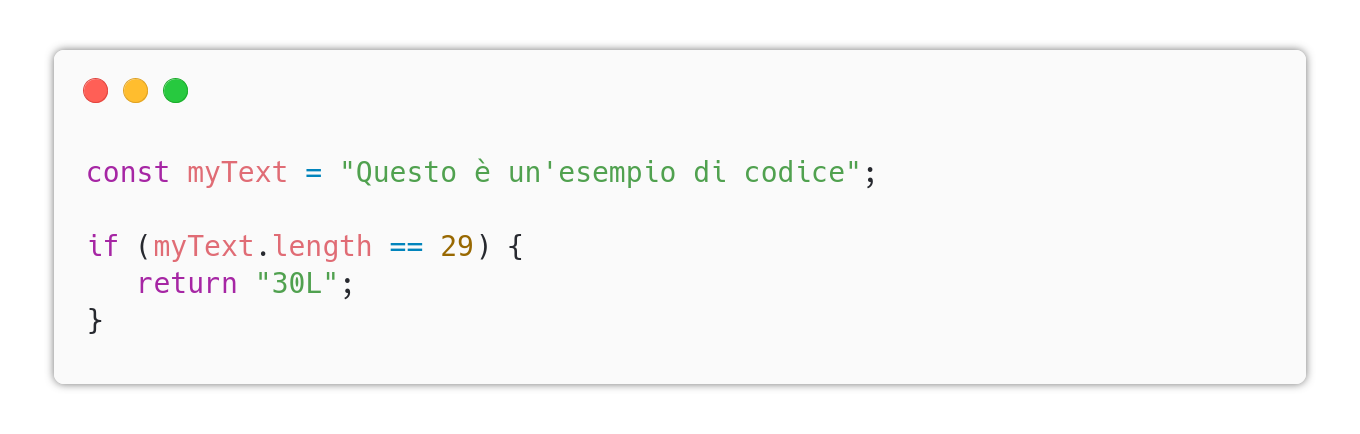
\includegraphics[width=1\textwidth]{images/example_code_01.png}
	Esempio di estratto di codice
\end{figure}

\section{Architettura dei Microservizi}

L'architettura proposta si basa sulla divisione logica (e fisica) delle funzionalità dell'applicazione tramite la distinzione di \textit{Microservizi}. Ciascun microservizio è indipendente dagli altri ed è composto a sua volta da una frontend e una backend distinte. Per tale ragione, è più accurato parlare di micro-frontend e micro-backend.

\subsection*{Vantaggi di un'architettura basata su microservizi}

Da un punto di vista di sviluppo, un'architettura non monolitica permette lo sviluppo asincrono dei singoli microservizi, oltre a facilitare la divisione del lavoro nelle varie parti. Tale architettura ha anche dei vantaggi a livello di performance in quanto il carico di lavoro chel'applicazione processa viene distribuito su più processi diminuendo il carico sul singolo. Altri vantaggi sono la scalarità dia una componente dell'applicazione in base alle esigenze e la ridondanza in quanto possono esistere più istanze di un microservizio contemporaneamente.

\subsection*{Svantaggi}

Un'architettura a microservizi è intrinsecamente più complessa nella progettazzione e nella menutenzione rispetto ad una architettura tradizionale. La necessità di orchestrare e mettere in comunicazione i diversi microservizi richiede particolari accortezze nella parte di design e di deploy. Tali problematiche sono state valutate con cura dal team di sviluppo.



\section{Visione Generale}
Prima di analizzare il singolo microservizio, questa sezione illustra una visione generale dell'applicazione e degli strumenti utilizzati per la realizzazione dell'infrastruttura, per poi concentrarsi sulle parti comuni di ogni microservizio e infine sul singolo microservizio.

\subsection{Tecnologie}

In questo capitolo verranno menzionate più volte alcune tecnologie, dunque ne viene riportata una breve descrizionee sotto:
\begin{itemize}
	\item "Docker": tecnologia che raccoglie il software in unità standardizzate chiamate container, offrendo tutto il necessario per la loro corretta esecuzione, incluse librerie, strumenti di sistema, codice e runtime. Il logo ricorda una balena di colore azzurro con dei rettangoli al di sopra rappresentanti dei containers, come se la balena stessa fosse una nave.
	\item "Docker Compose": software per la gestione di molteplici docker containers contemporaneamente. L'icona rappresenta un polpo con dei parallelepipedi azzurri tra i tentacoli.
	\item "Nginx": intermediario tra le richieste da parte dei client e il server. Può essere usato come load balancer, cache o proxy. Il logo è raffigurato da un N bianca con sfondo verde.
	\item "MongoDB": DBMS non relazionale. Il logo rappresenta una foglia verde.
	\item "Express": framework backend per applicazioni web in javascript. Il logo è formato dalle due lettere "e" e "x" in nero.
	\item "React": framework frontend lo sviluppo di applicazioni web. L'icona ricorda un atomo.
\end{itemize}

\subsection{Specifica dell'Infrastruttura}

Si presti attenzione alla seguente infografica dell'infrastruttura implementata:

\begin{figure}[H]
	\centering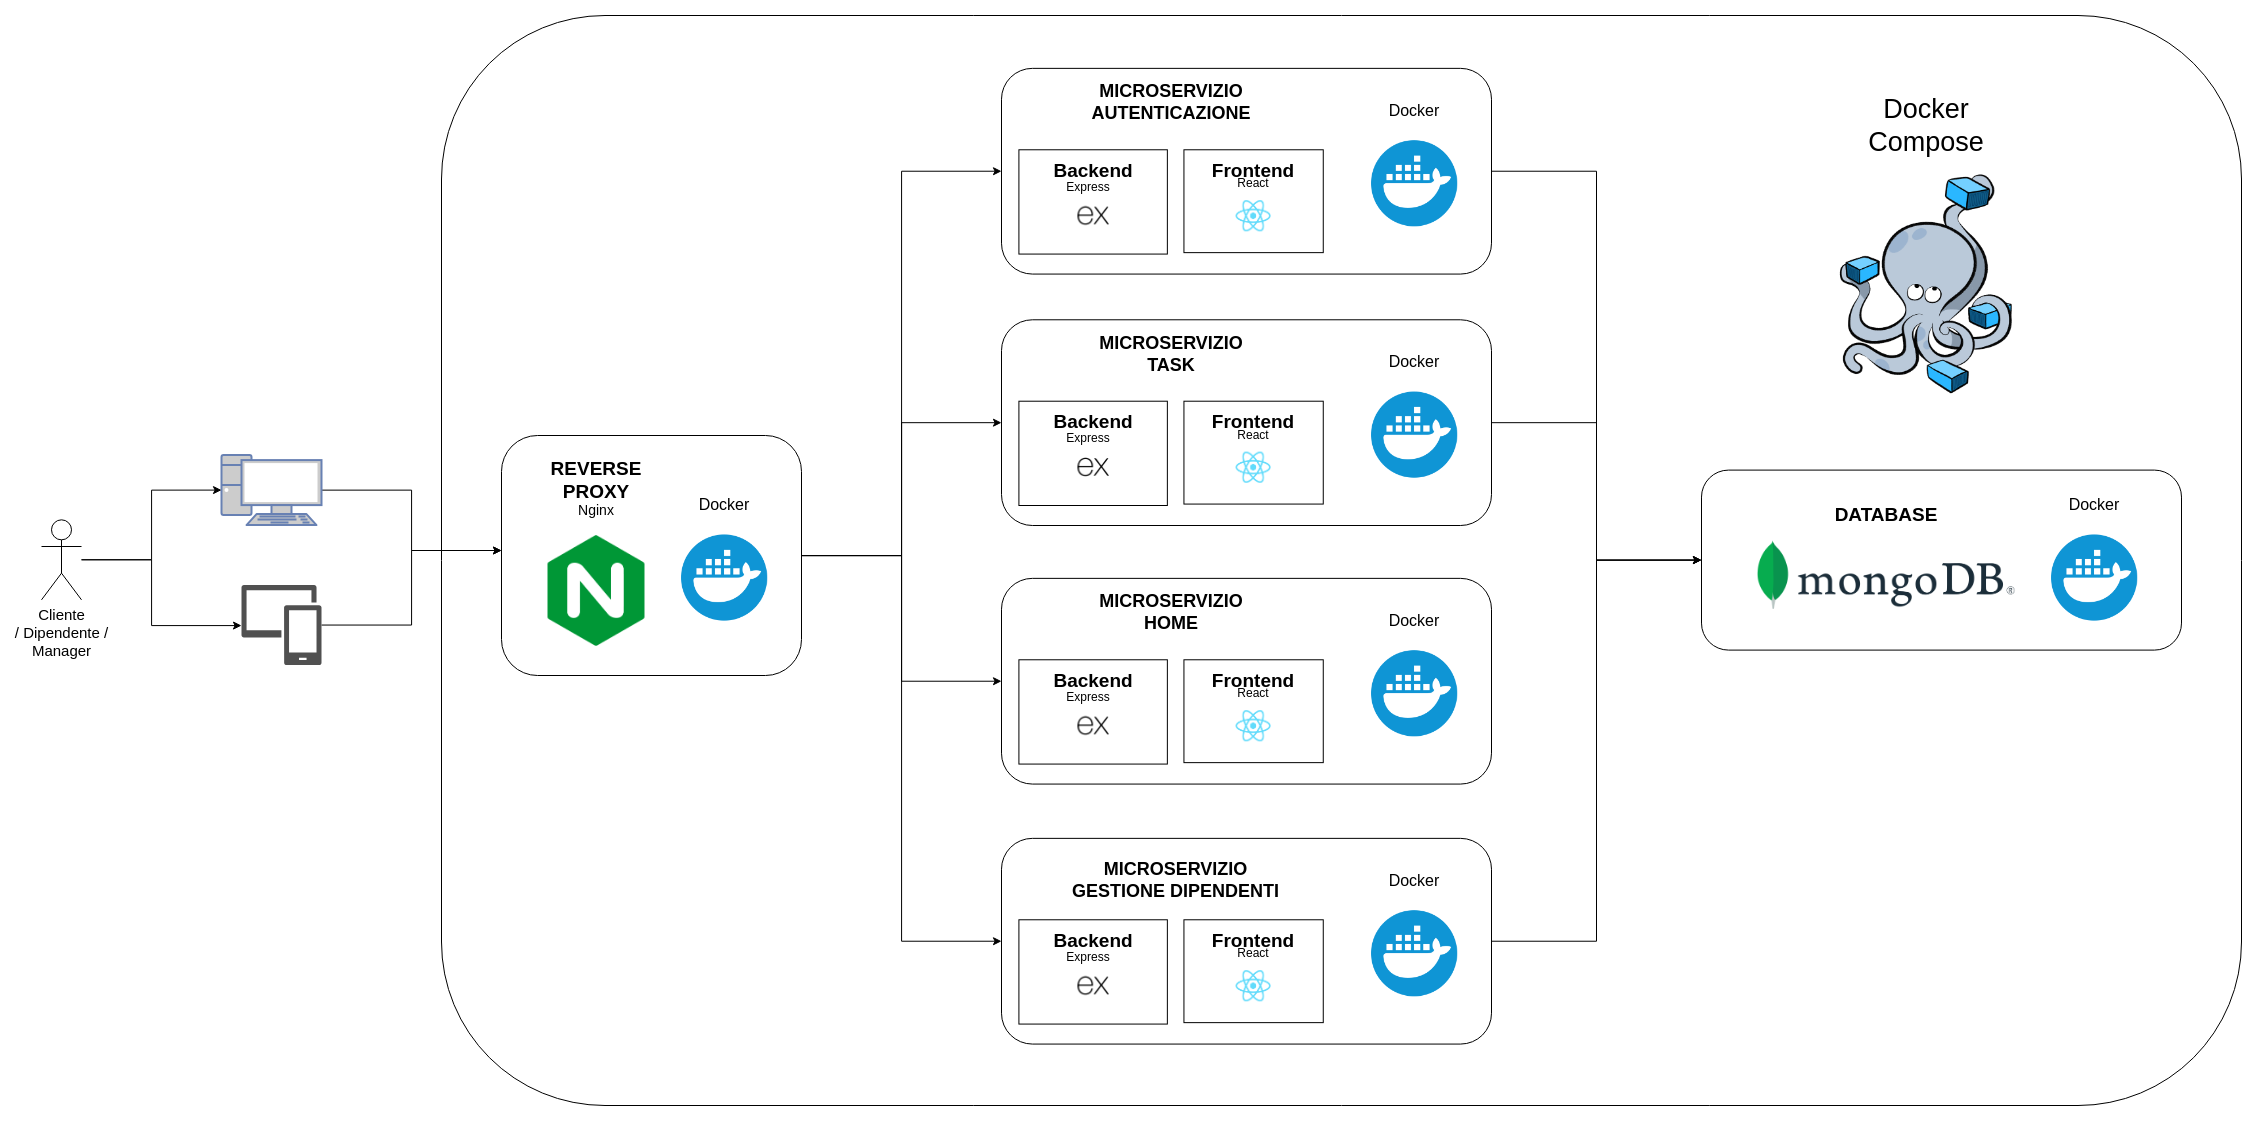
\includegraphics[width=1\textwidth]{images/diagramma_microservizi.png}
	Schema dei microservizi
\end{figure}

L'intera infrastruttura viene inizializzata con \textit{Docker Compose}. In particolare, \textit{Docker Compose} si occupa di impostare i containers sullo stesso network con un IP statico e le variabili di ambiente come le porte e gli IP dei rispettivi microservizi, oltre ad inizializzare i containers, le porte e volumi condivisi.

Se eseguito su un singolo host, il network di default segue la seguente struttura:
\begin{figure}[H]
	\centering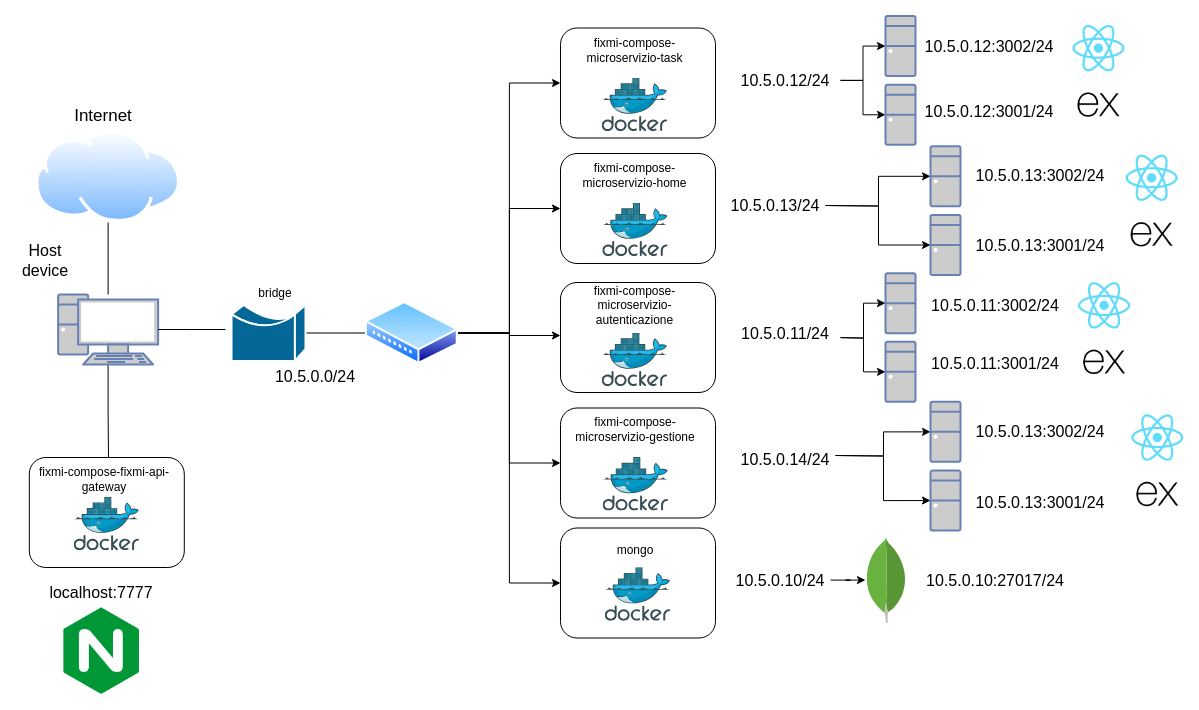
\includegraphics[width=1\textwidth]{images/network.png}
	Schema del network dei microservizi
\end{figure}

Docker imposta i microservizi sul network 10.5.0.0/24 con i seguenti IP:
% table
\begin{center} % center the table
	\centering
	\begin{tabular}{ |p{4cm}|p{4cm}|  }
		\hline
		\centering Nome Microservizio     & \qquad\quad Network IP \\ % I found no other way...
		\hline
		MongoDB                           & 10.5.0.10/24           \\
		\hline
		Microservizio Autenticazione      & 10.5.0.11/24           \\
		\hline
		Microservizio Task                & 10.5.0.12/24           \\
		\hline
		Microservizio Home                & 10.5.0.13/24           \\
		\hline
		Microservizio Gestione Dipendenti & 10.5.0.14/24           \\
		\hline
		Reverse Proxy                     & 127.0.0.1              \\
		\hline
	\end{tabular}
\end{center}

Ad ogni servizio sono state assegnate le seguenti porte:

\begin{center} % center the table
	\centering
	\begin{tabular}{ |p{4cm}|p{4cm}|  }
		\hline
		\centering Nome servizio & \qquad\qquad Porta \\ % I found no other way...
		\hline
		MongoDB                  & 27017              \\
		\hline
		Backend                  & 3001               \\
		\hline
		frontend                 & 3002               \\
		\hline
		Reverse Proxy            & 7777               \\
		\hline
	\end{tabular}
\end{center}

Due microservizi particolari sono il database e il reverse proxy. Il database fornisce la possibilità di salvare in modo permanente i dati dell'applicazione, mentre il reverse proxy permette di accedere facilmente all'ip di un microservizio attraverso una mappatura di ip. I software scelti sono rispettivamente \textit{MongoDB} e \textit{Nginx}.

In particolare, \textit{Nginx} associa le routes nel seguente modo:
\begin{figure}[H]
	\centering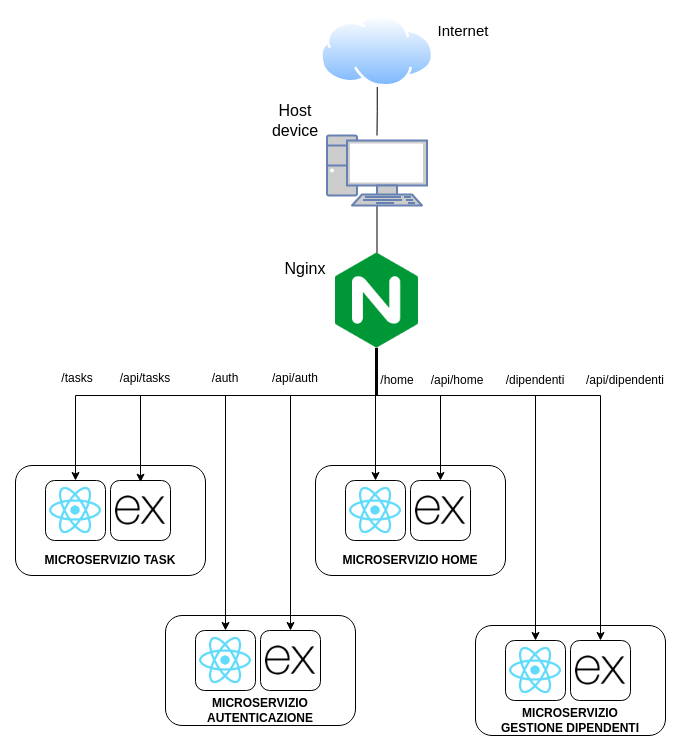
\includegraphics[width=1\textwidth]{images/nginx.png}
	Schema delle routes di Nginx
\end{figure}

\section{Codice}
In questa sezione verrà mostrato il codice che implementa quanto sopra, con opportuna spiegazione del funzionamento quando necessaria.

\subsection{Codice: Struttura}

La directory radice del progetto contiene i seguenti files:

\begin{figure}[H]
	\centering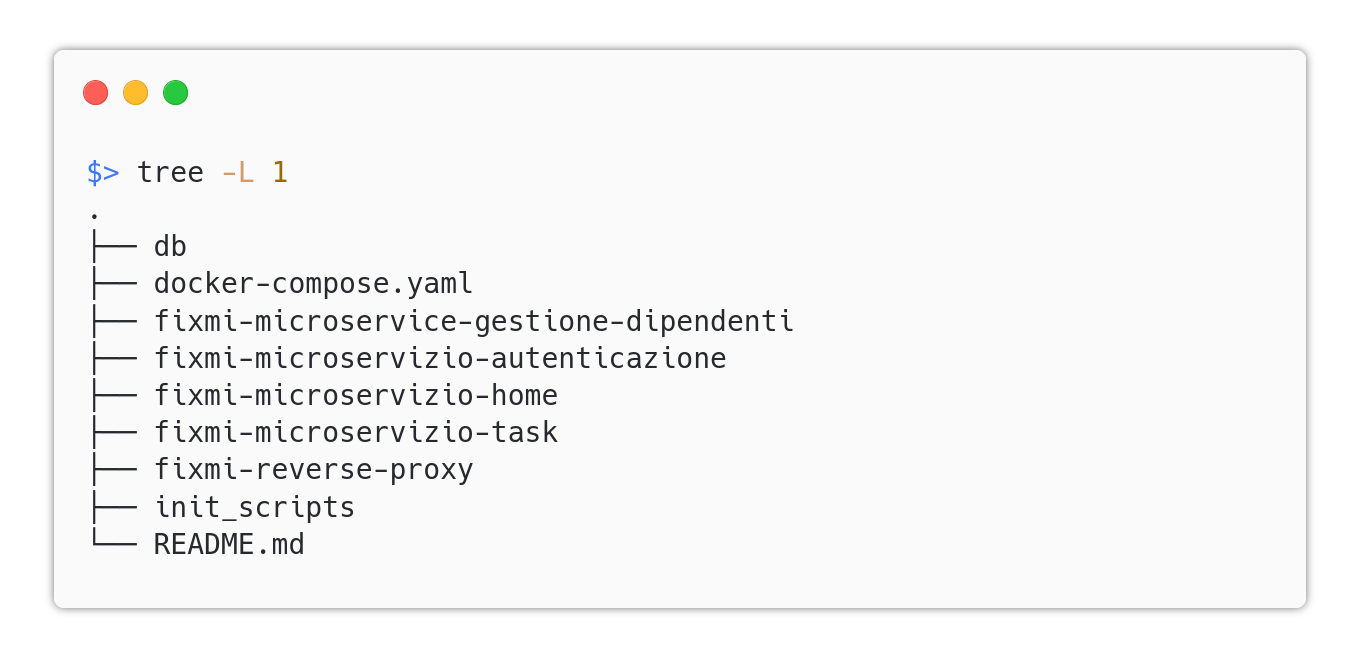
\includegraphics[width=1\textwidth]{images/tree.png}
	Output del comando "tree", mostra i contenuti della directory root del progetto.
\end{figure}

Segue una descrizione degli stessi:
\begin{itemize}
	\item "db": volume condiviso tra il docker container del database e il filesystem dell'host per mantenere persistenza dei dati quando il container viene riavviato o rimosso.
	\item "docker-compose.yaml": file di configurazione utilizzato da docker compose per inizializzare l'infrastruttura. Contiene le informazioni per avviare gli altri microservizi.
	\item "fixmi-microservice-gestione-dipendenti": cartella contenente il microservizio "Gestione Dipendenti".
	\item "fixmi-microservizio-autenticazione": cartella contenente il microservizio "Autenticazione".
	\item "fixmi-microservizio-home": cartella contenente il microservizio "Home".
	\item "fixmi-microservizio-task": cartella contenente il microservizio "task".
	\item "fixmi-reverse-proxy": cartella contenente il reverse proxy.
	\item "init\_scripts": script per inizializzare il database con dei dati di esempio.
	\item "README.md": contiene informazioni e documentazione sul deploy dell'infrastruttura.
\end{itemize}

\subsection{Codice: docker-compose.yaml}

Si prenda come esempio questo frammento di codice responsabile del setup del microservizio task:
\begin{figure}[H]
	\centering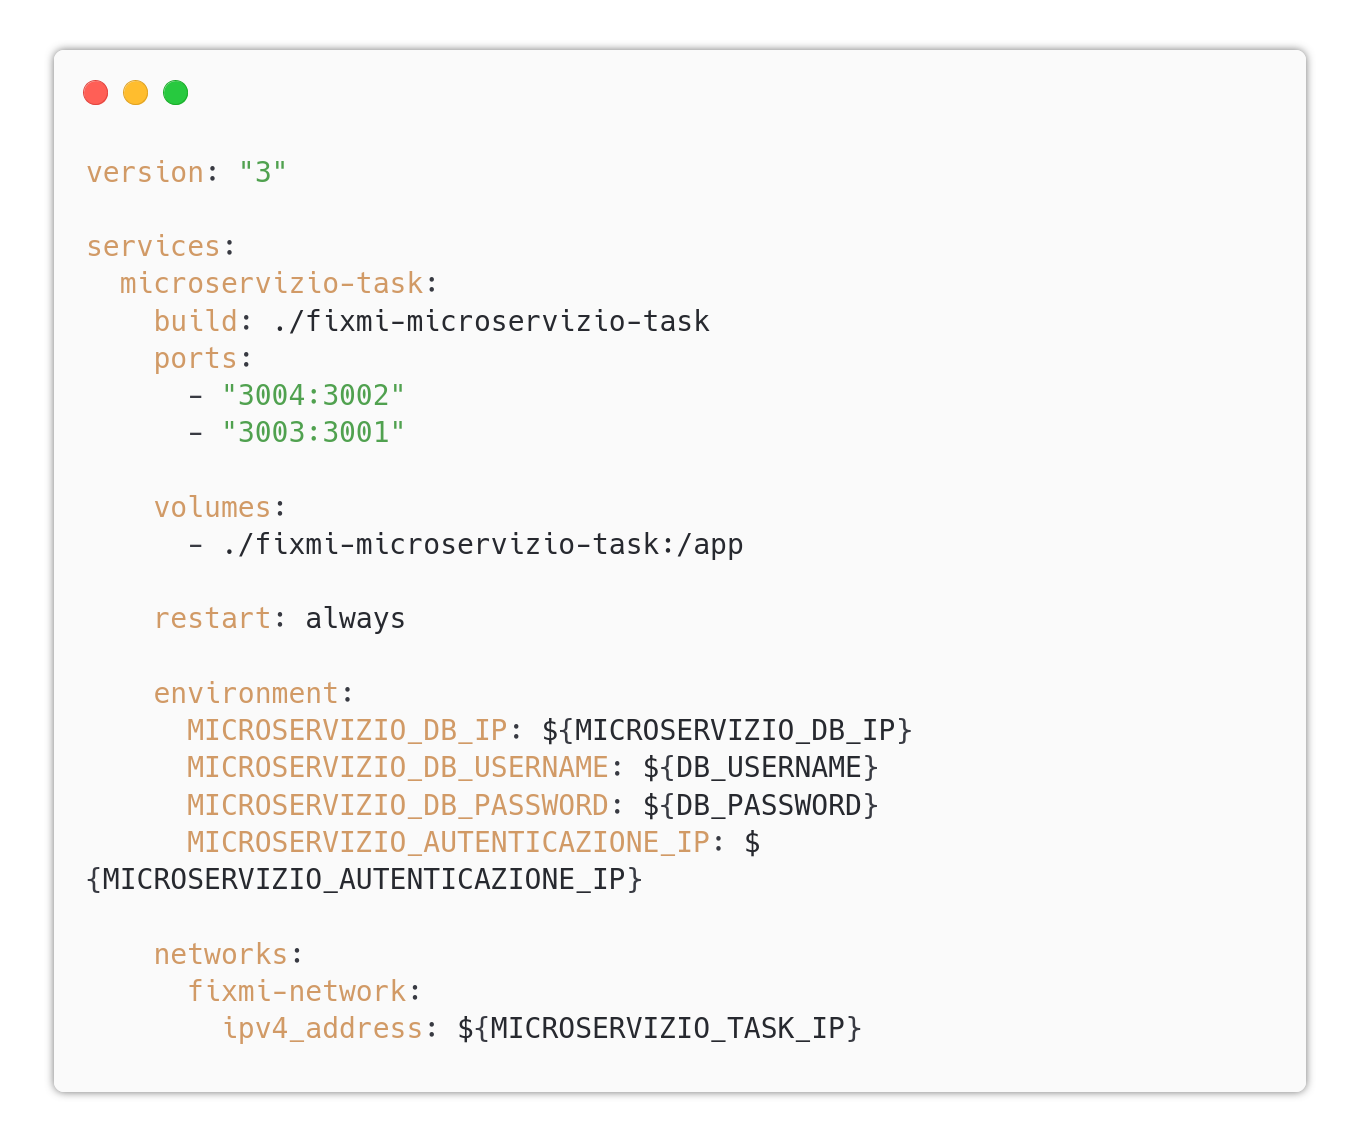
\includegraphics[width=1\textwidth]{images/docker_code_01.png}
	Estratto dal file "docker-compose.yaml"
\end{figure}

In questo codice, notiamo che le porte vengono impostate sotto la sezione "ports", così come i volumi e il network. Le variabili d'ambiente contenenti i vari ip e le credenziali del database sono contenute nel file ".env" presente nella radice della cartella.
La configurazione per gli altri microservizi è simile, con qualche piccola differenza. Qua sotto vengono riportati gli altri microservizi:
\begin{figure}[H]
	\centering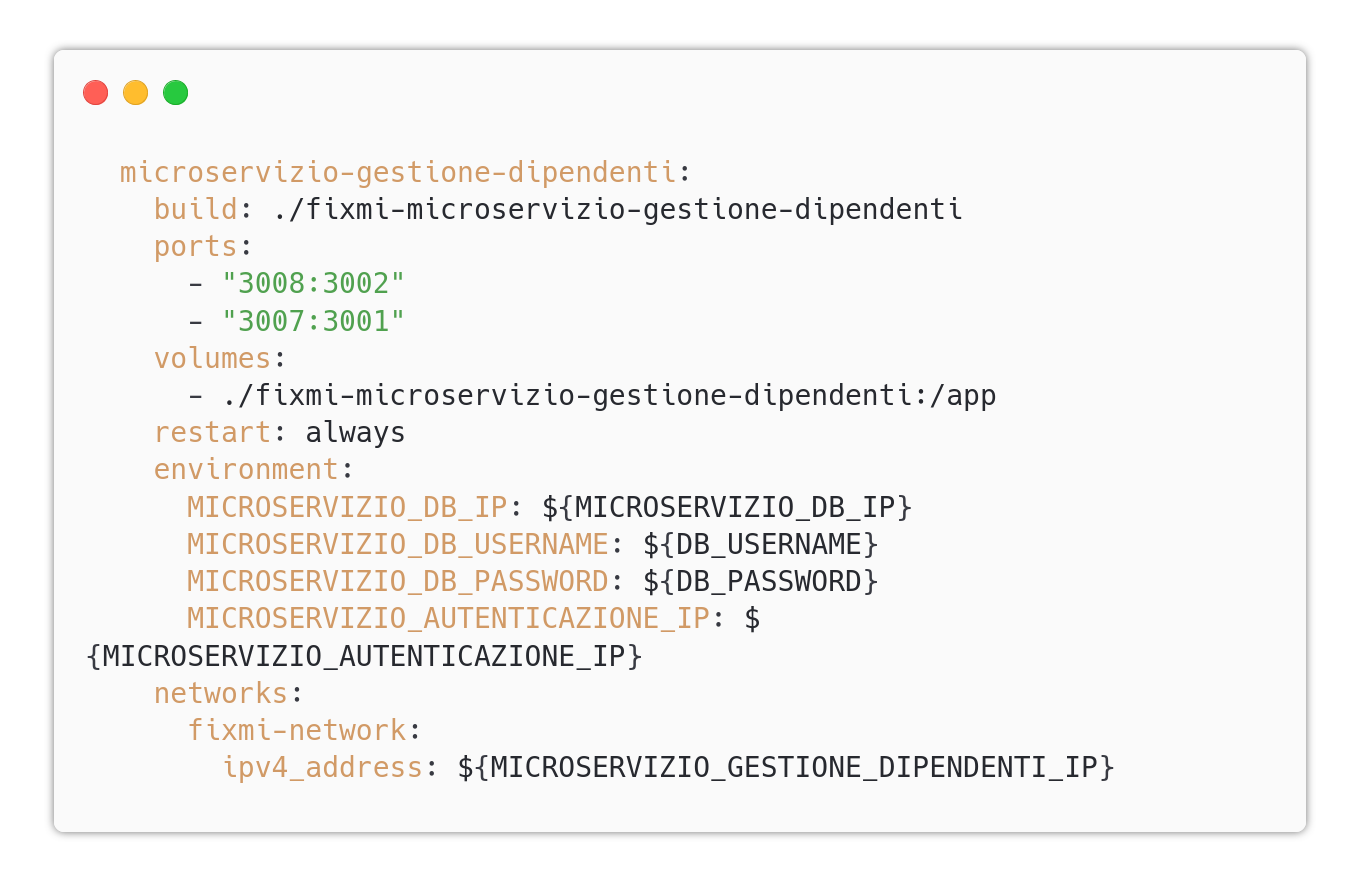
\includegraphics[width=1\textwidth]{images/yaml_gestione_dipendenti.png}
	Codice responsabile per l'avvio del microservizio "Gestione Dipendenti"
\end{figure}
\begin{figure}[H]
	\centering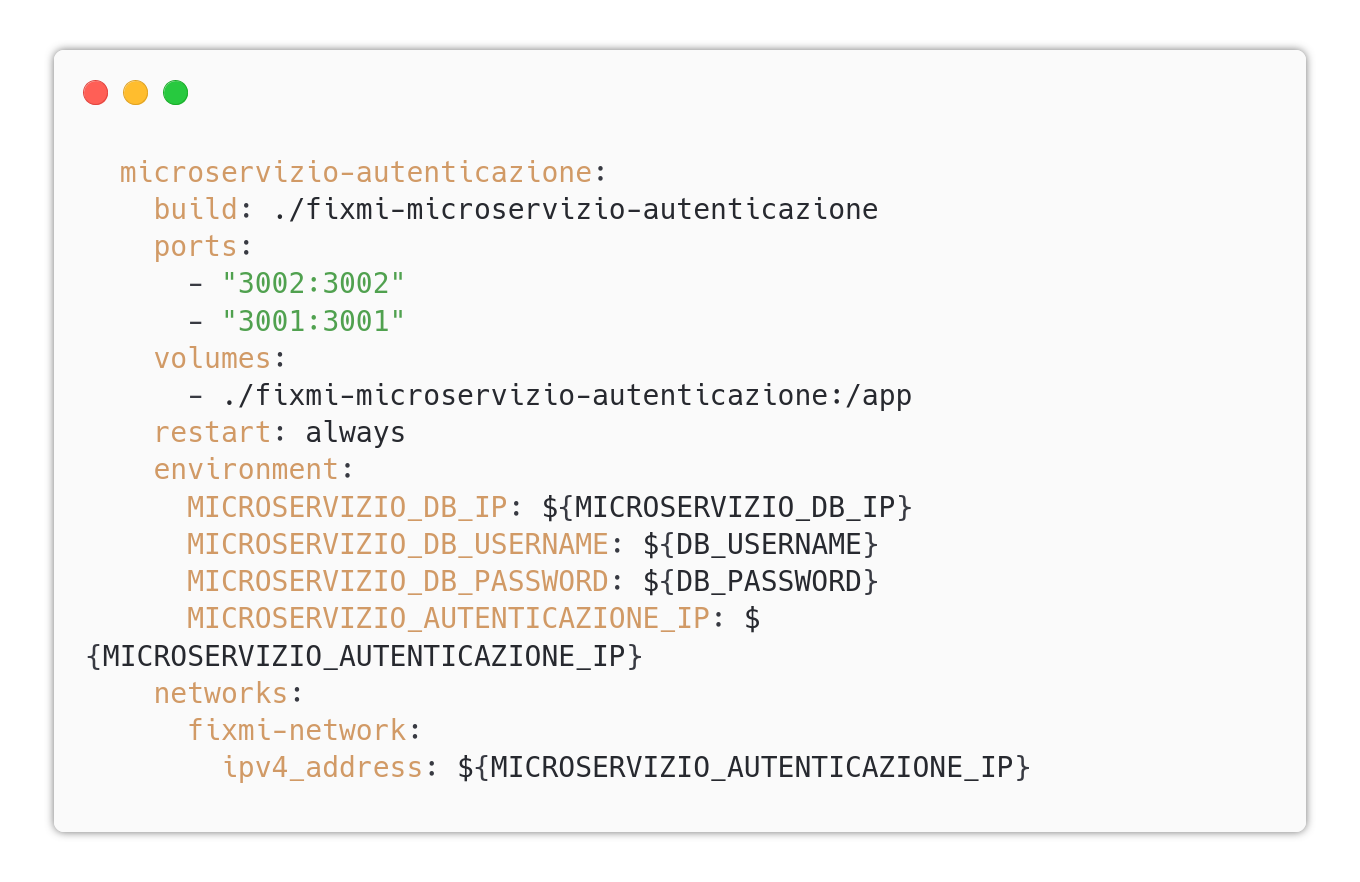
\includegraphics[width=1\textwidth]{images/yaml_autenticazione.png}
	Codice responsabile per l'avvio del microservizio "Autenticazione"
\end{figure}
\begin{figure}[H]
	\centering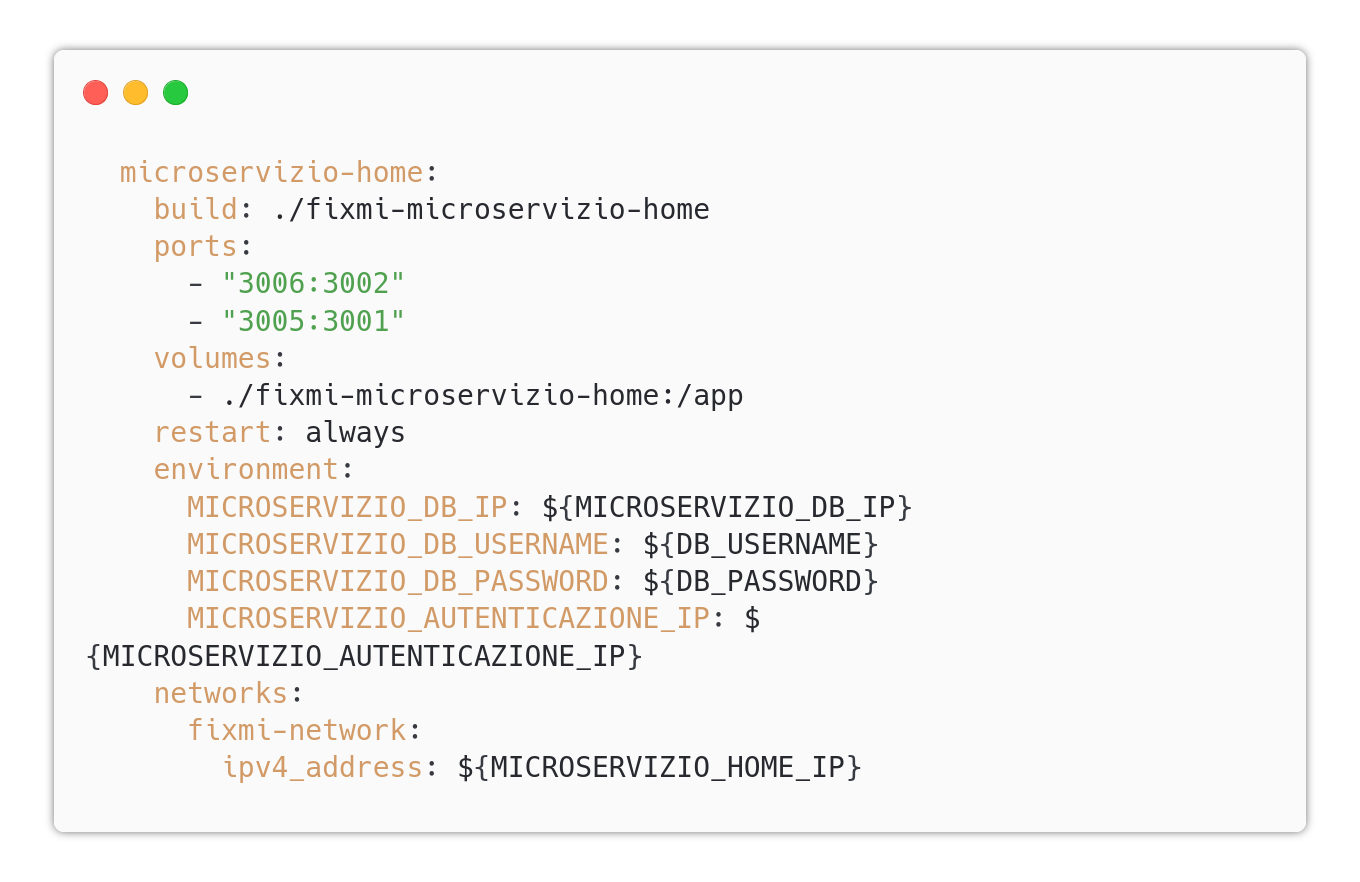
\includegraphics[width=1\textwidth]{images/yaml_home.png}
	Codice responsabile per l'avvio del microservizio "Home"
\end{figure}
\begin{figure}[H]
	\centering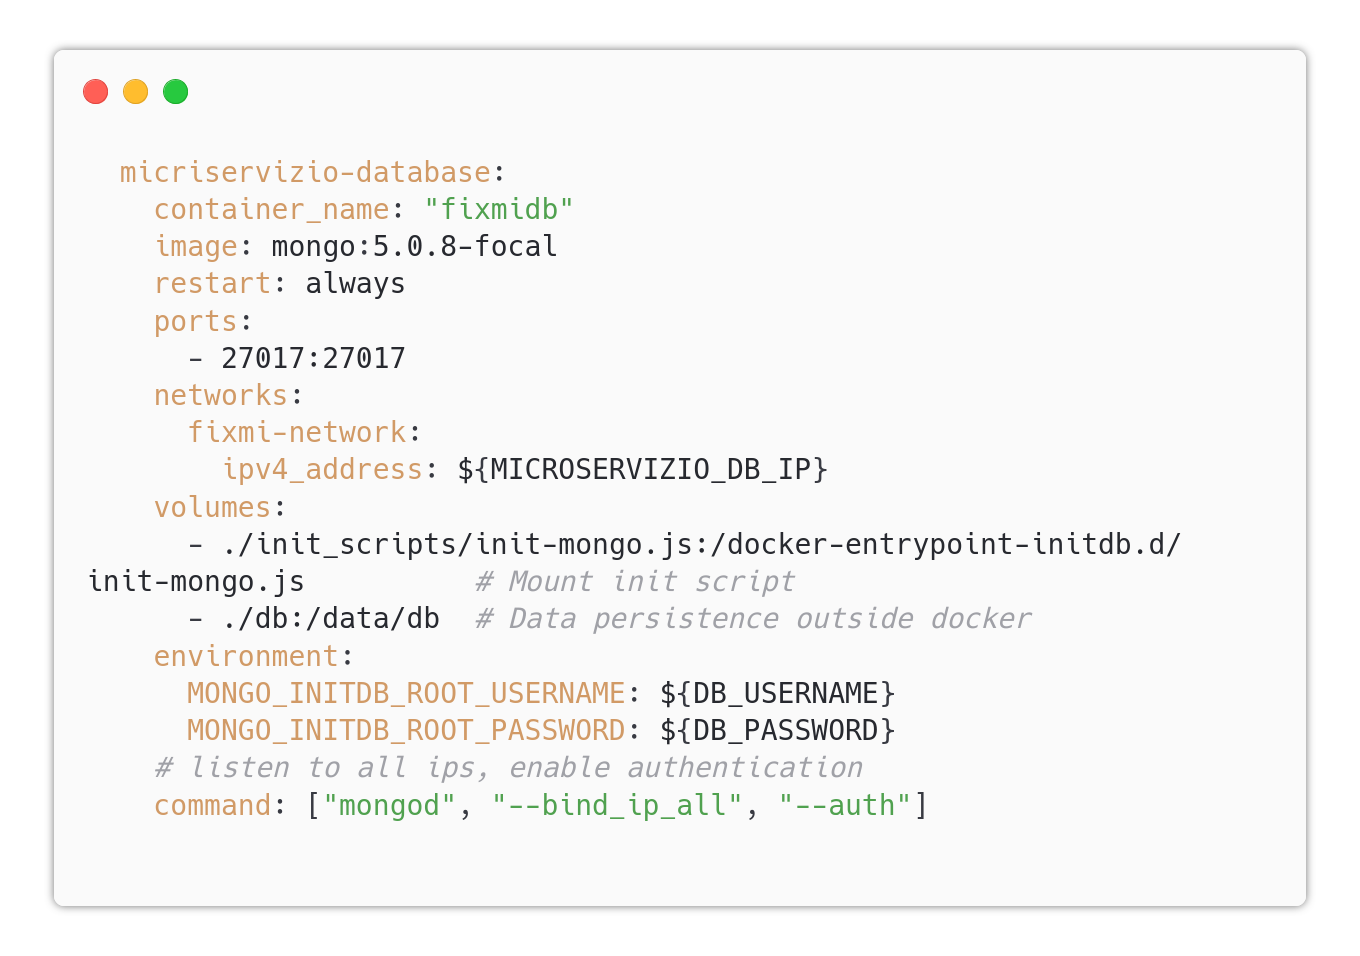
\includegraphics[width=1\textwidth]{images/yaml_database.png}
	Codice responsabile per l'avvio del database
\end{figure}
\begin{figure}[H]
	\centering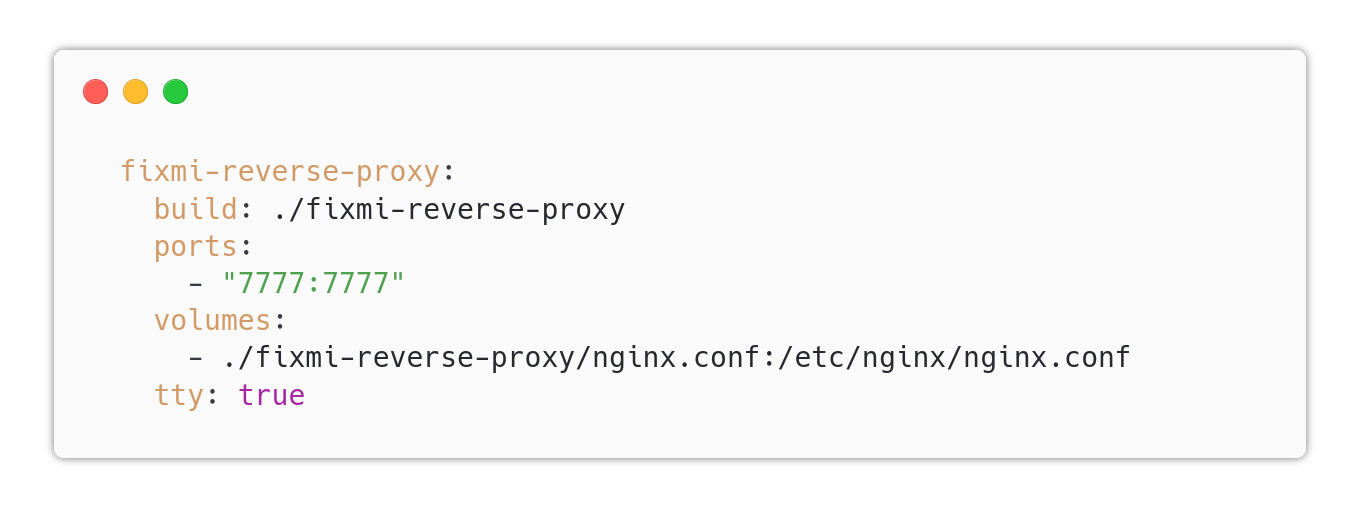
\includegraphics[width=1\textwidth]{images/yaml_reverse_proxy.png}
	Codice responsabile per l'avvio del reverse proxy
\end{figure}

\subsection{Codice: nginx.conf}

Il file \textit{nginx.conf} all'interno della cartella \textit{fixmi-reverse-proxy} imposta la configurazione per il reverse proxy. Questo microservizio si occupa di instradare le richieste ai vari microservizi. Segue un'estratto della configurazione:


\begin{figure}[H]
	\centering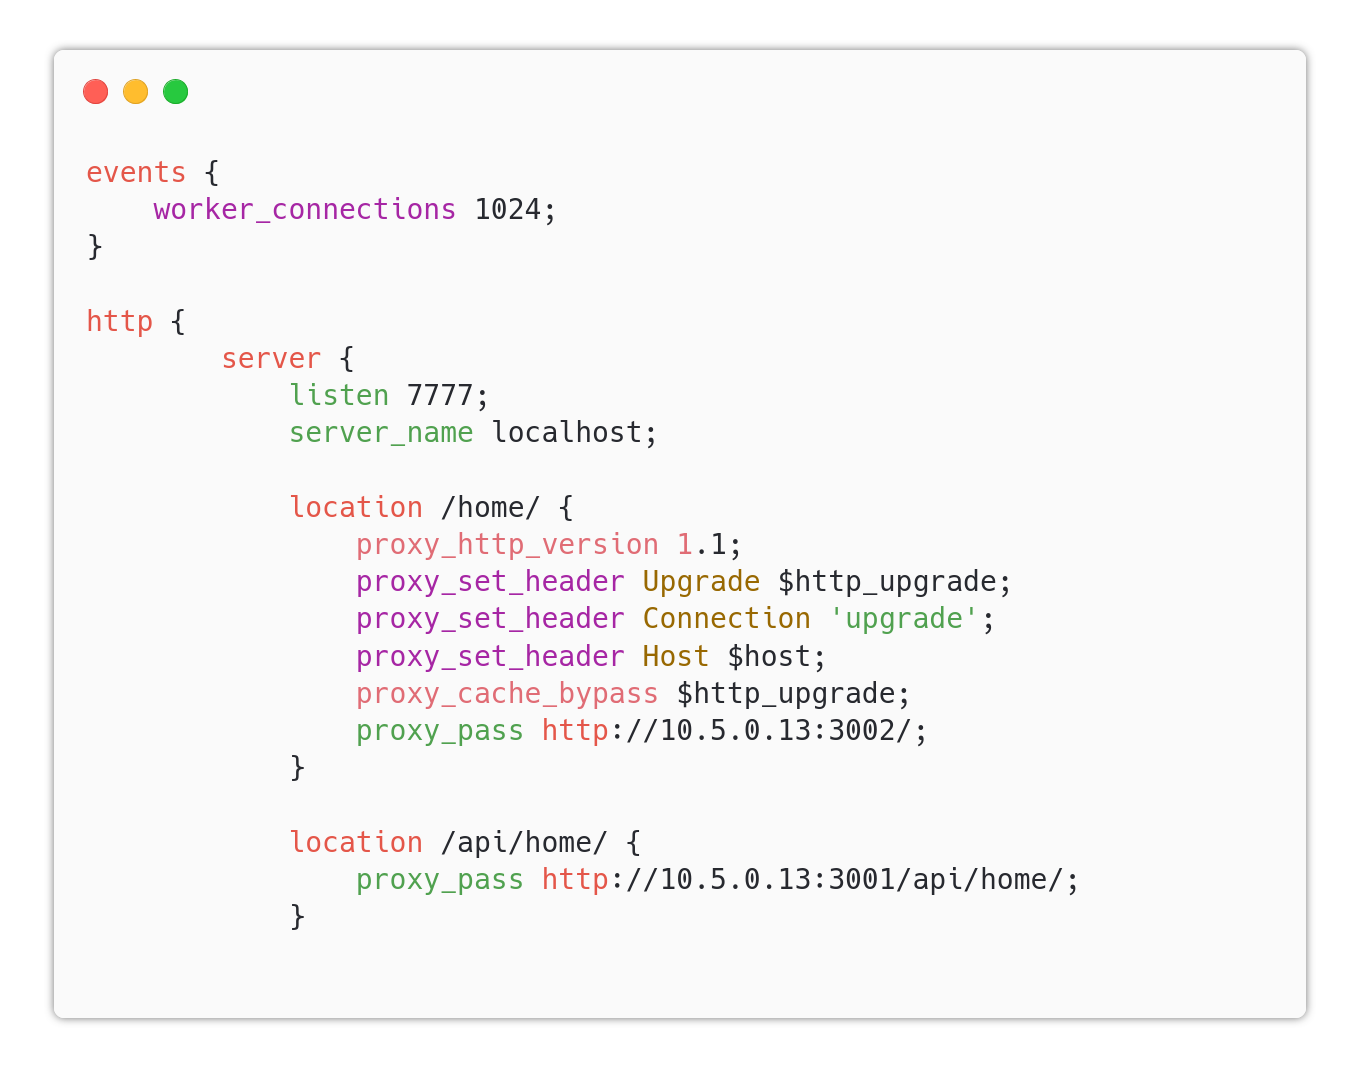
\includegraphics[width=1\textwidth]{images/nginx_config_home.png}
	Estratto da "fixmi-reverse-proxy/nginx.conf", definizione delle routes "/home" e "/api/home"
\end{figure}

La variabile "worker\_connections" definisce il numero di connessioni simultanee che il servizio può gestire. Il blocco "http" e il blocco "server" contengono le configurazioni delle routes, in particolare in questo esempio notiamo che la route "/home/" viene passata a "http://10.5.0.13:3002/" ossia la frontend del microservizio "home", mentre "/api/home/" rimanda a "http://10.5.0.13:3001/api/home/" ossia la backend del microservizio "home". Vengono inoltre impostati alcuni headers dopo la dicitura "proxy\_set\_header".

Di seguito vengono riportate le altre routes:

\begin{figure}[H]
	\centering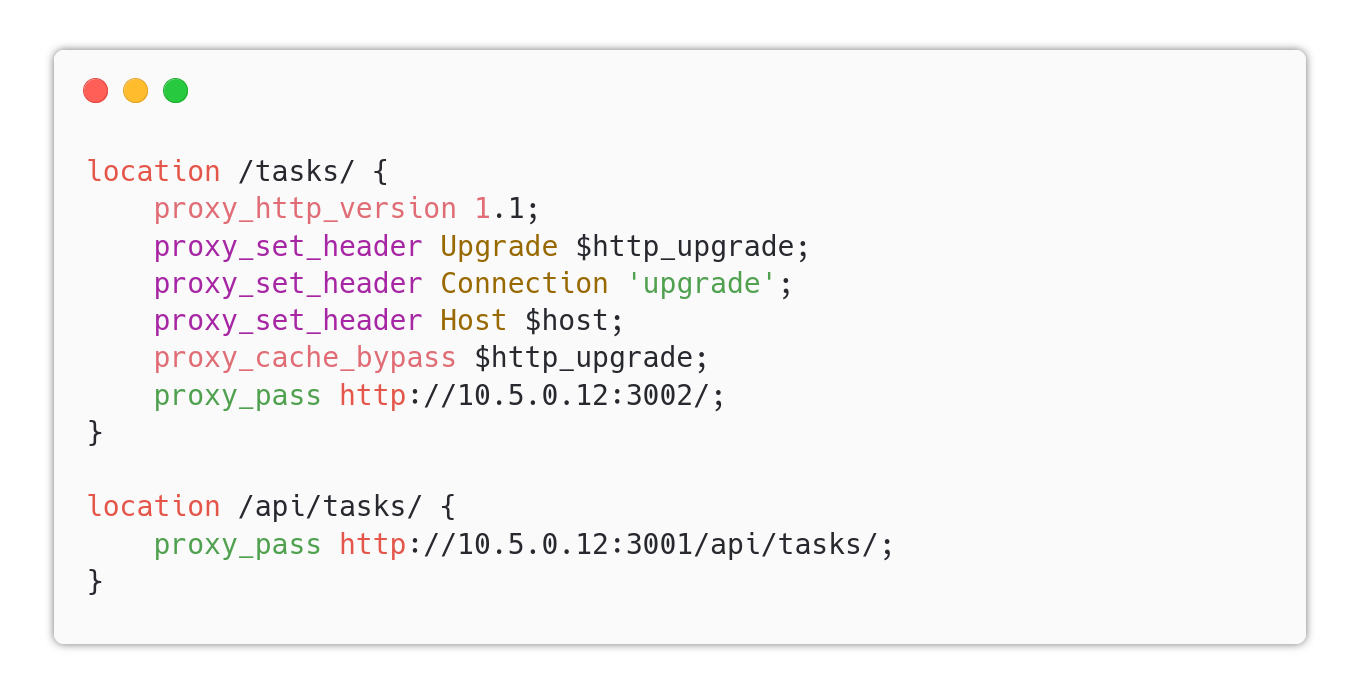
\includegraphics[width=1\textwidth]{images/nginx_config_tasks.png}
	Routes "/tasks" e "/api/tasks"
\end{figure}
\begin{figure}[H]
	\centering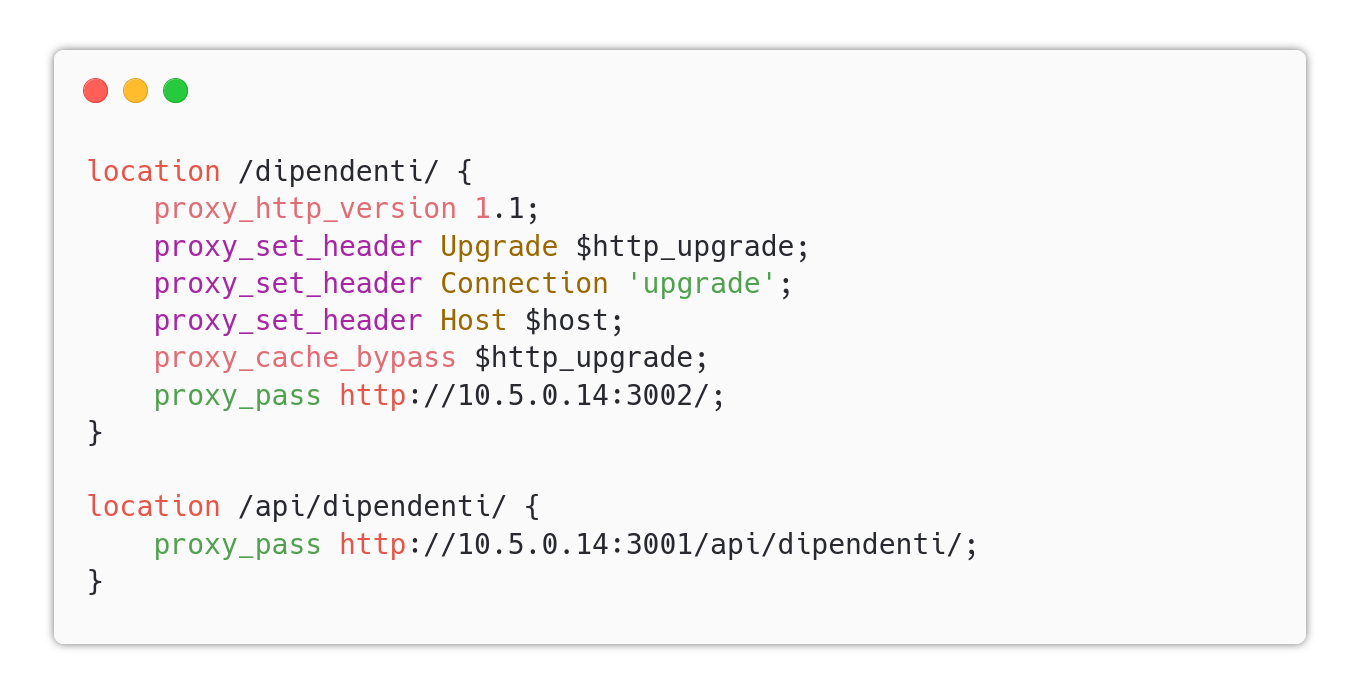
\includegraphics[width=1\textwidth]{images/nginx_config_dipendenti.png}
	Routes "/dipendenti" e "/api/dipendenti"
\end{figure}
\begin{figure}[H]
	\centering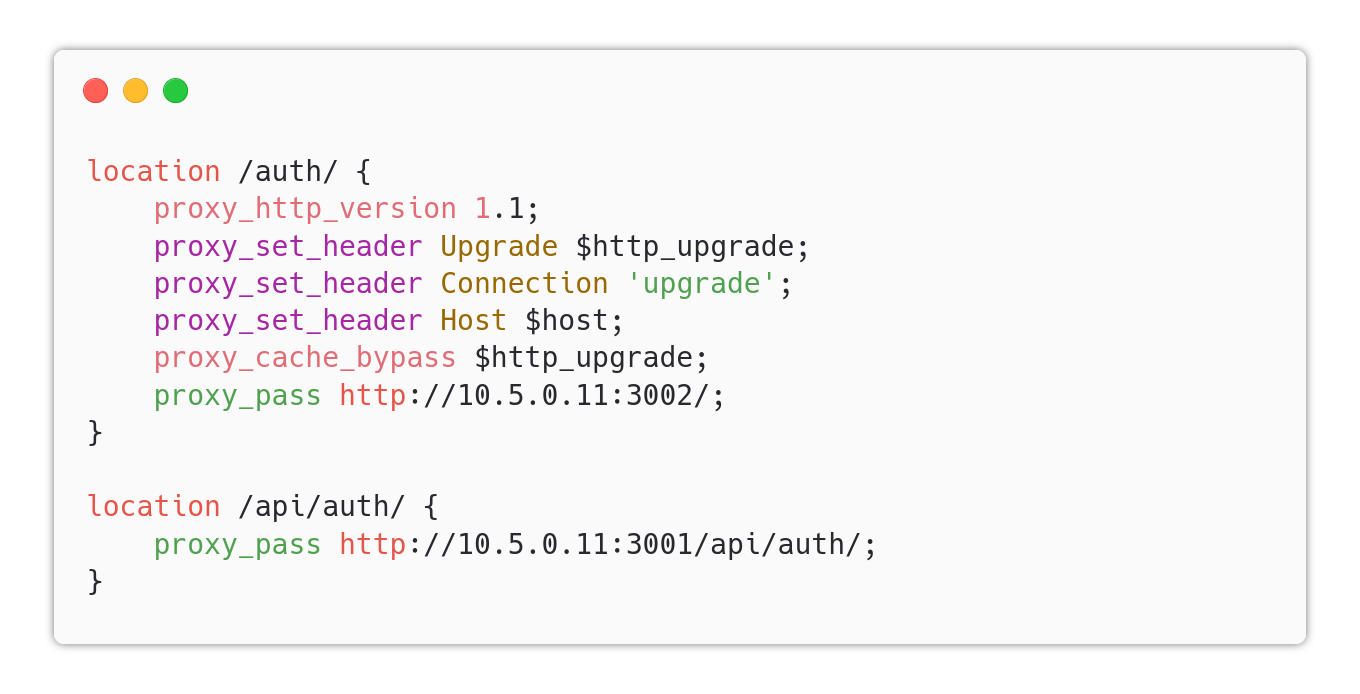
\includegraphics[width=1\textwidth]{images/nginx_config_auth.png}
	Routes "/auth" e "/api/auth"
\end{figure}

\subsection*{Codice: init-mongo.js}

Il file contiene l'inizializzazione delle entrate del database in formato json. Sono stati individuati due database: "Tasks" e "Users" e le rispettive collezioni "tasks" e "users" (da notare la differenza della prima lettera da maiuscola a minuscola). I contenuti sono i seguenti:
\begin{figure}[H]
	\centering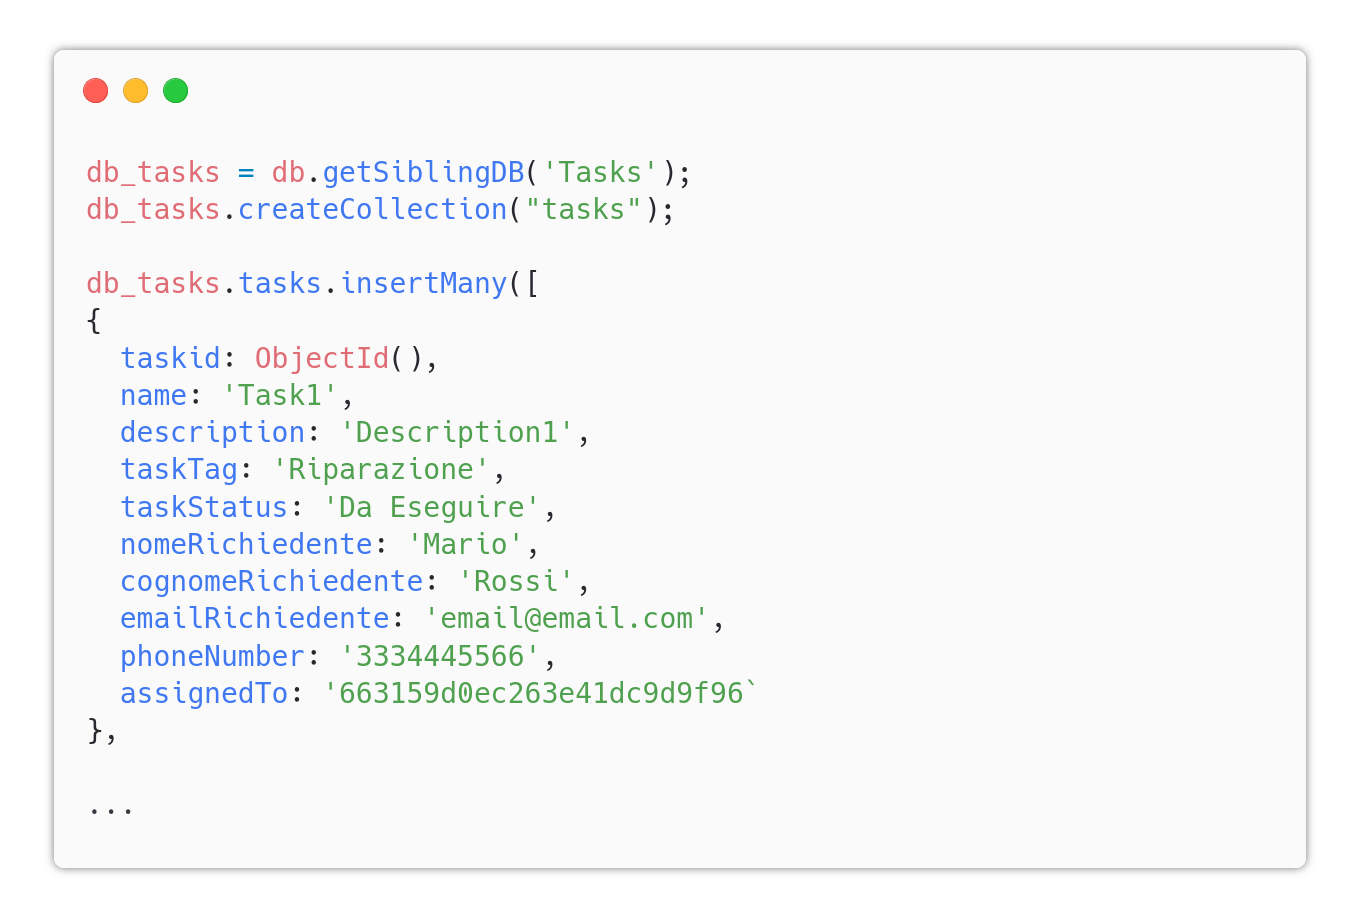
\includegraphics[width=1\textwidth]{images/db-tasks.png}
	Inizializzazione database "Task"
\end{figure}

\begin{figure}[H]
	\centering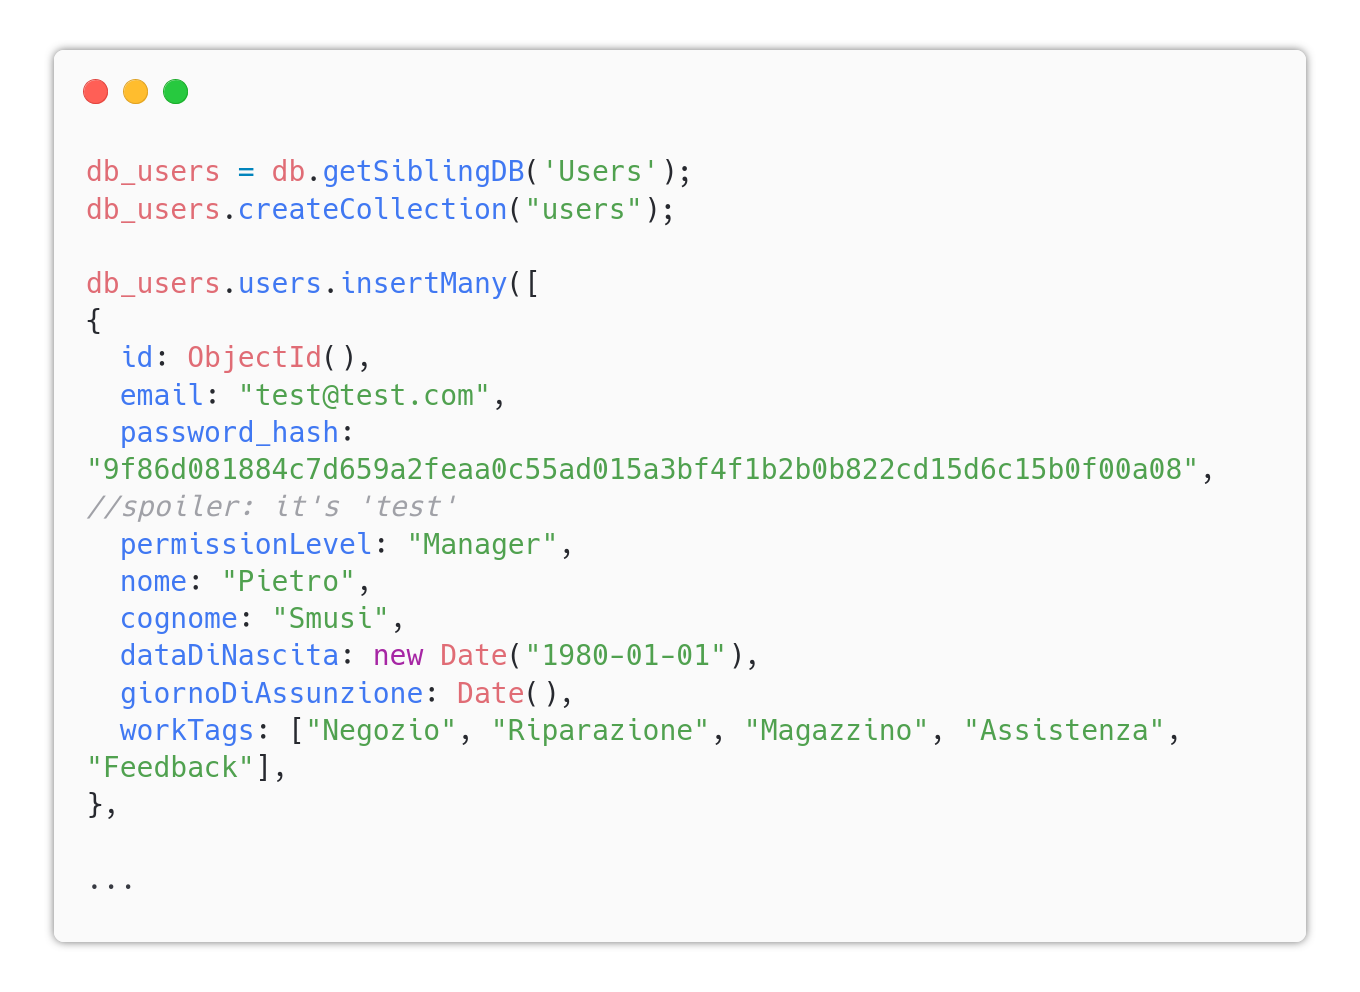
\includegraphics[width=1\textwidth]{images/db-users.png}
	Inizializzazione database "Users"
\end{figure}


\section{Parti comuni ad ogni microservizio}

In questa sezione verrà descritta la struttura che accomuna i vari microservizi.

\subsection{Scelta del Linguaggio}

Il linguaggio scelto per la backend e frontend è \textit{Typescript}: un linguaggio tipizzato che viene tradotto da un compilatore ("transpiler") in Javascript e dunque può essere eseguito in un web browser. Qualsiasi script JavaScript è anche codice TypeScript valido, questo permette all'applicazione di utilizzare l'ampia collezione di pacchetti JavaScript.

\subsection{Frameworks e Dipendenze}

Ogni microservizio utilizza:
\begin{itemize}
	\item \textit{ts-node} v10.9.2: ambiente runtime Typescript open source e multipiattaforma per la creazione del server di backend.
	\item \textit{eslint} v8.56.0: analizzatore di codice statico.
	\item \textit{nodemon} v3.0.3: tool di assistenza per Node.js. permette il riavvio automatico del server quando viene rilevata una modifica nel codice.
	\item \textit{express} v4.18.2: framework web per Node.js, utilizzato per la realizzazione di api.
	\item \textit{React} v18.3.0: libreria UI per javascript, utilizzata per la frontend.
	\item \textit{tailwindcss} v3.4.1: framework CSS.
	\item \textit{Jest} v29.7.0 : framework per il testing
	\item \textit{supertest} v7.0.0: framework per il testing di api, utilizzato insieme a Jest.
	\item \textit{concurrently} v8.2.2: esegue più comandi contemporaneamente, utilizzato per eseguire frontend e backend insieme.
	\item \textit{serve} v14.2.3: hosta un sito statico, utilizzato per hostare la frontend in produzione.
	\item \textit{dotenv} v16.4.5: permette l'accesso alle variabili di ambiente, utilizzate per la configurazione dei microservizi.
	\item \textit{body-parser} v1.20.2: permette di leggere il body di una richiesta http.
	\item \textit{mongodb} v6.5.0: interfaccia per la connessione al microservizio database.
\end{itemize}

\subsection{Struttura}

La cartella di un microservizio presenta i seguenti files:
\begin{figure}[H]
	\centering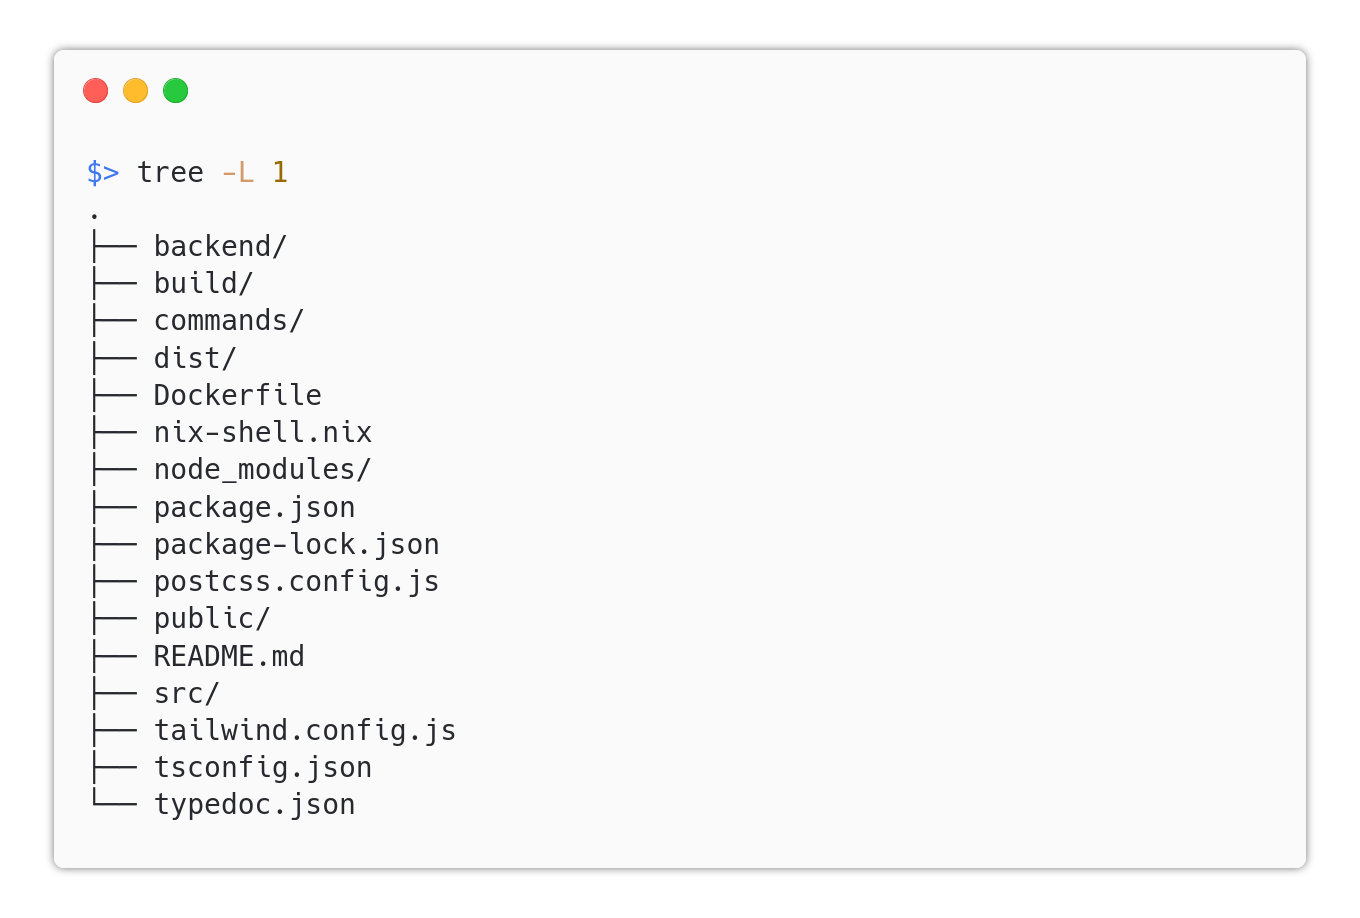
\includegraphics[width=1\textwidth]{images/structure.png}
	Output del comando "tree" all'interno di un microservizio.
\end{figure}
Segue una descrizione degli stessi, dall'alto verso il basso:
\begin{itemize}
	\item "backend": cartella contenente tutto il codice di Backend in TypeScript.
	\item "build": cartella contenente l'applicazione web statica generata da React.
	\item "commands": cartella contenente degli appunti degli sviluppatori durante la creazione del progetto.
	\item "dist": cartella contenente il codice backend per la produzione, generato dal compilatore di TypeScript.
	\item "Dockerfile": file contenente le istruzioni per la generazione del contenitore di docker.
	\item "nix-shell.nix": file contenente l'ambiente di sviluppo per chi sviluppa su NixOS.
	\item "node\_modules/": cartella contenente i moduli utilizzati dall'applicazione
	\item "package.json": file che definise le dipendenze e le impostazioni di vari moduli.
	\item "package-lock.json": contiene le versioni delle dipendenze dei moduli.
	\item "postcss.config.js": script di configurazione necessario per tailwindcss
	\item "public": contiene file di accesso pubblico per la frontned, come favicon.ico, robots.txt, index.html.
	\item "README.md": contiene le informazioni del progetto e le istruzioni per il deploy.
	\item "src/": cartella contenente tutto il codice per la frontend in tsx.
	\item "tailwind.config.js": file di configurazione per il funzionamento di tailwindcss
	\item "tsconfig.json": configurazione per TypeScript.
\end{itemize}


\subsubsection*{Directory backend/}

\begin{figure}[H]
	\centering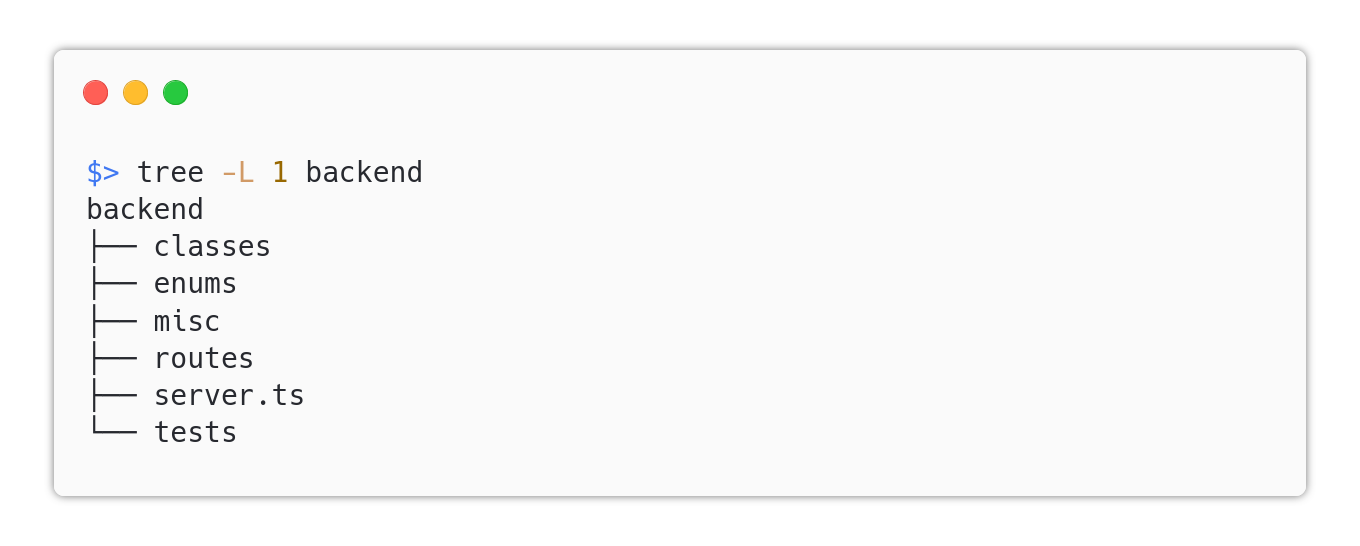
\includegraphics[width=1\textwidth]{images/tree_backend.png}
	Output del comando "tree" all'interno della cartella "backend/".
\end{figure}


La struttura della directory "backend/" segue il seguente formato:
\begin{itemize}
	\item server.ts: è il file principale. Si occupa di istanziare l'App di express,
	      connettersi al database e definire le route delle API.
	\item classes/ : directory contenente le classi relative ai profili, che vengono manipolate ed immagazzinate nel database.
	\item enums/ : directory contenente gli enumi necessari.
	\item routes/ : directory contenente gli endpoint delle API del sistema.
	\item tests/ : directory contenente i test delle API
	\item utils/ : directory contenente strutture dati e funzioni utili al funzionamento del sistema.
\end{itemize}

\subsection{Comandi npm}
Vengono definiti i seguenti scripts per l'esecuzione dell'applicazione tramite npm. Ogni comando può esssere eseguito digitando "npm run" ed il nome del comando.
\begin{itemize}
	\item "startfront": esegue solo la frontend, si aggiorna automaticamente ad ogni modifica del codice
	\item "buildfront": genera la frontend statica per la production
	\item "startback": esegue soltanto il server di backend, si aggiorna automaticamente ad ogni modifica del codice
	\item "start": esegue sia la frontend sia la backend in developement mode
	\item "production": esegue sia la frontend sia la backend in production mode
	\item "lint": esegue un'analisi stica del codice
	\item "test": esegue gli script di testing del codice.
\end{itemize}

\subsection{Elementi frontend}
Ogni microservizio condivide due componenti grafici, "navbar.tsx" e "footer.tsx" posizionati sempre rispettivamente in cima e in fondo ad ogni pagina dell'applicazione.
Il loro scopo è rendere la navigazione per l'utente più semplice e chiara
\subsubsection{Navbar}
\begin{figure}[H]
	\centering
\includegraphics[width=1\textwidth]{images/navbar.jpg}
	\caption{Immagine del componente "navbar.tsx"}
\end{figure}
Contiene bottoni per accedere ai diversi microservizi del sito, ha uno stile ed un design semplice ed intuitivo in linea con il resto dell'applicazione.
\begin{figure}[H]
	\centering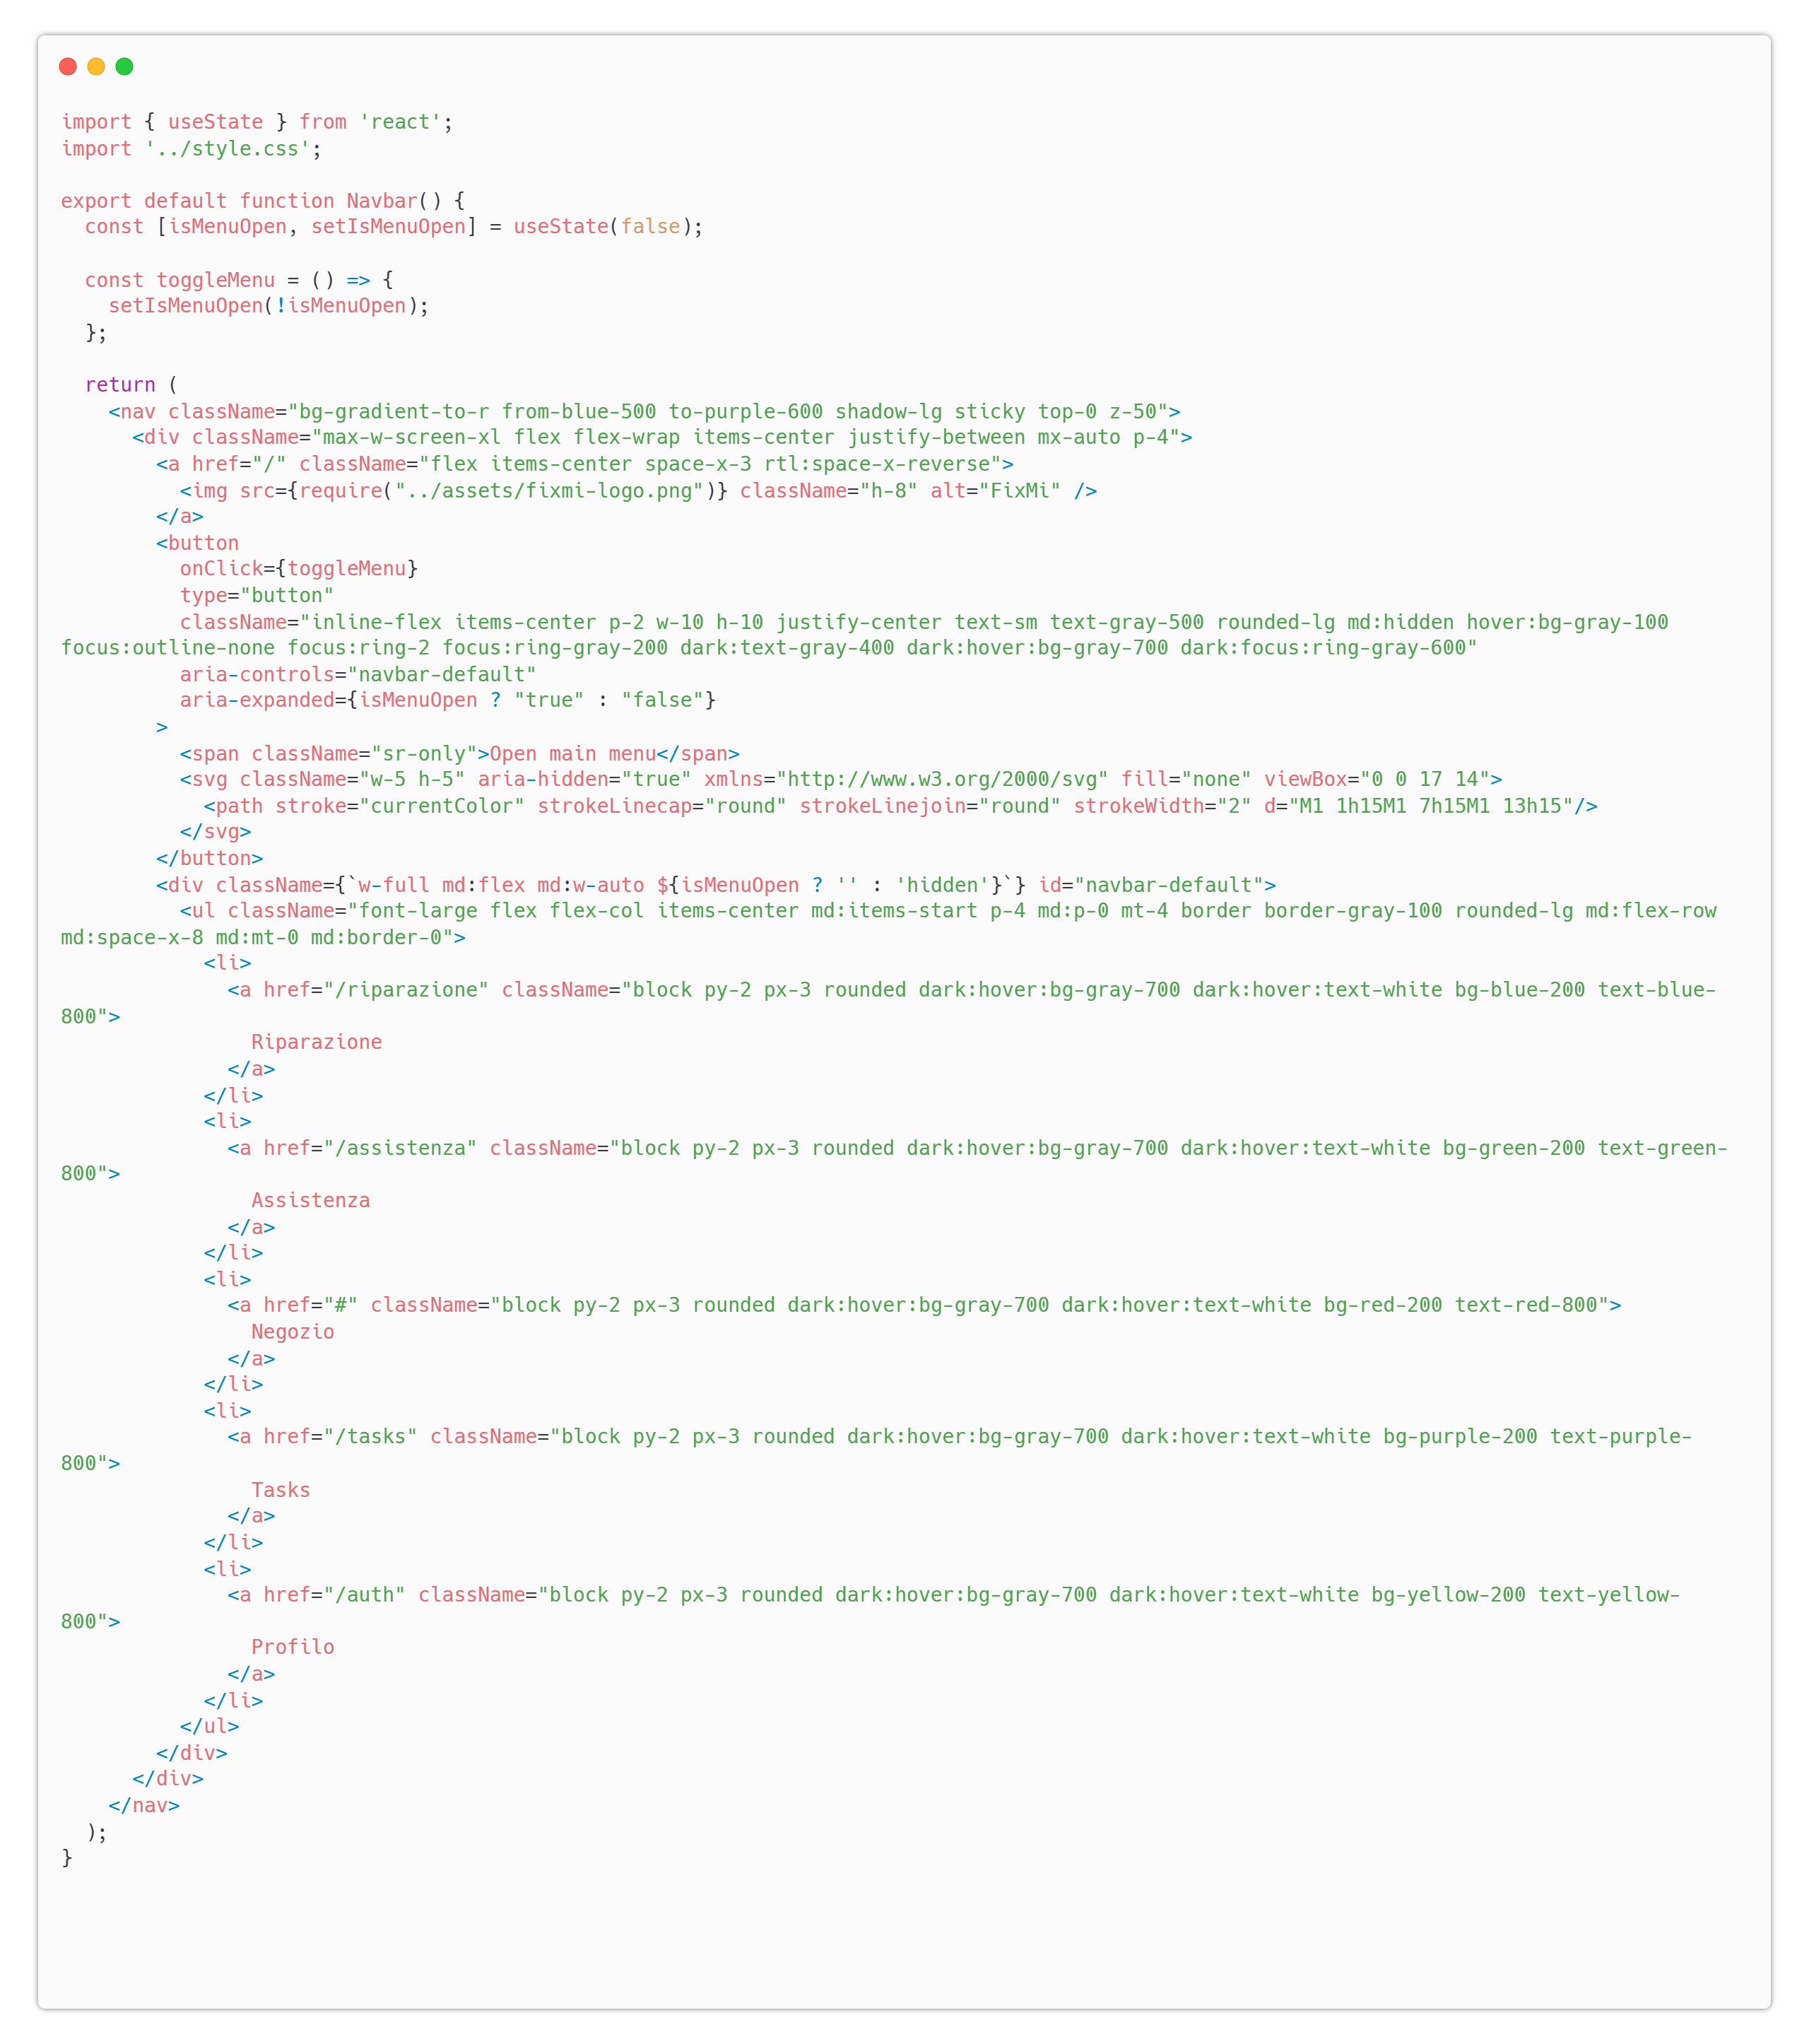
\includegraphics[width=1\textwidth]{images/navbar-carbon.png}
	\caption{Codice del componente "navbar.tsx"}
\end{figure}
\subsubsection{Footer}
\begin{figure}[H]
	\centering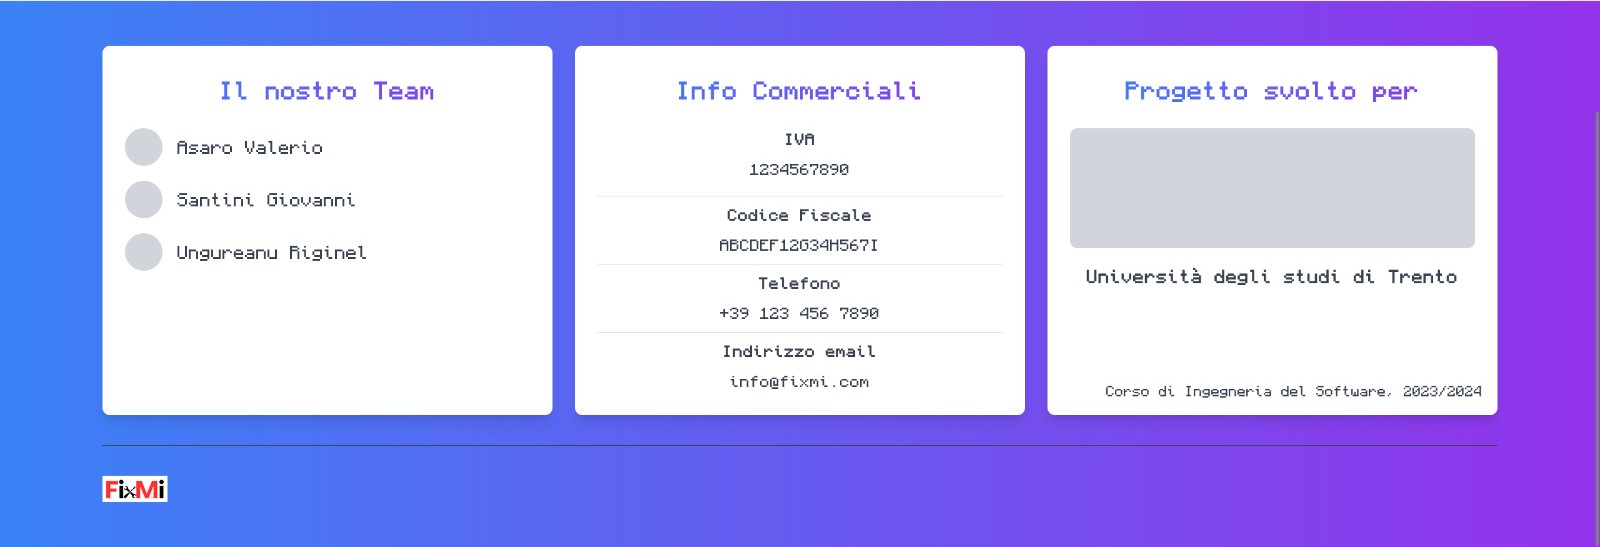
\includegraphics[width=1\textwidth]{images/footer.jpg}
	\caption{Immagine del componente "footer.tsx"}
\end{figure}
Contiene le principali informazioni sugli autori dell'applicazione "FixMi", dell'azienda e contatti di cui l'utente potrebbe eventualmente avere bisogno 
\begin{figure}[H]
	\centering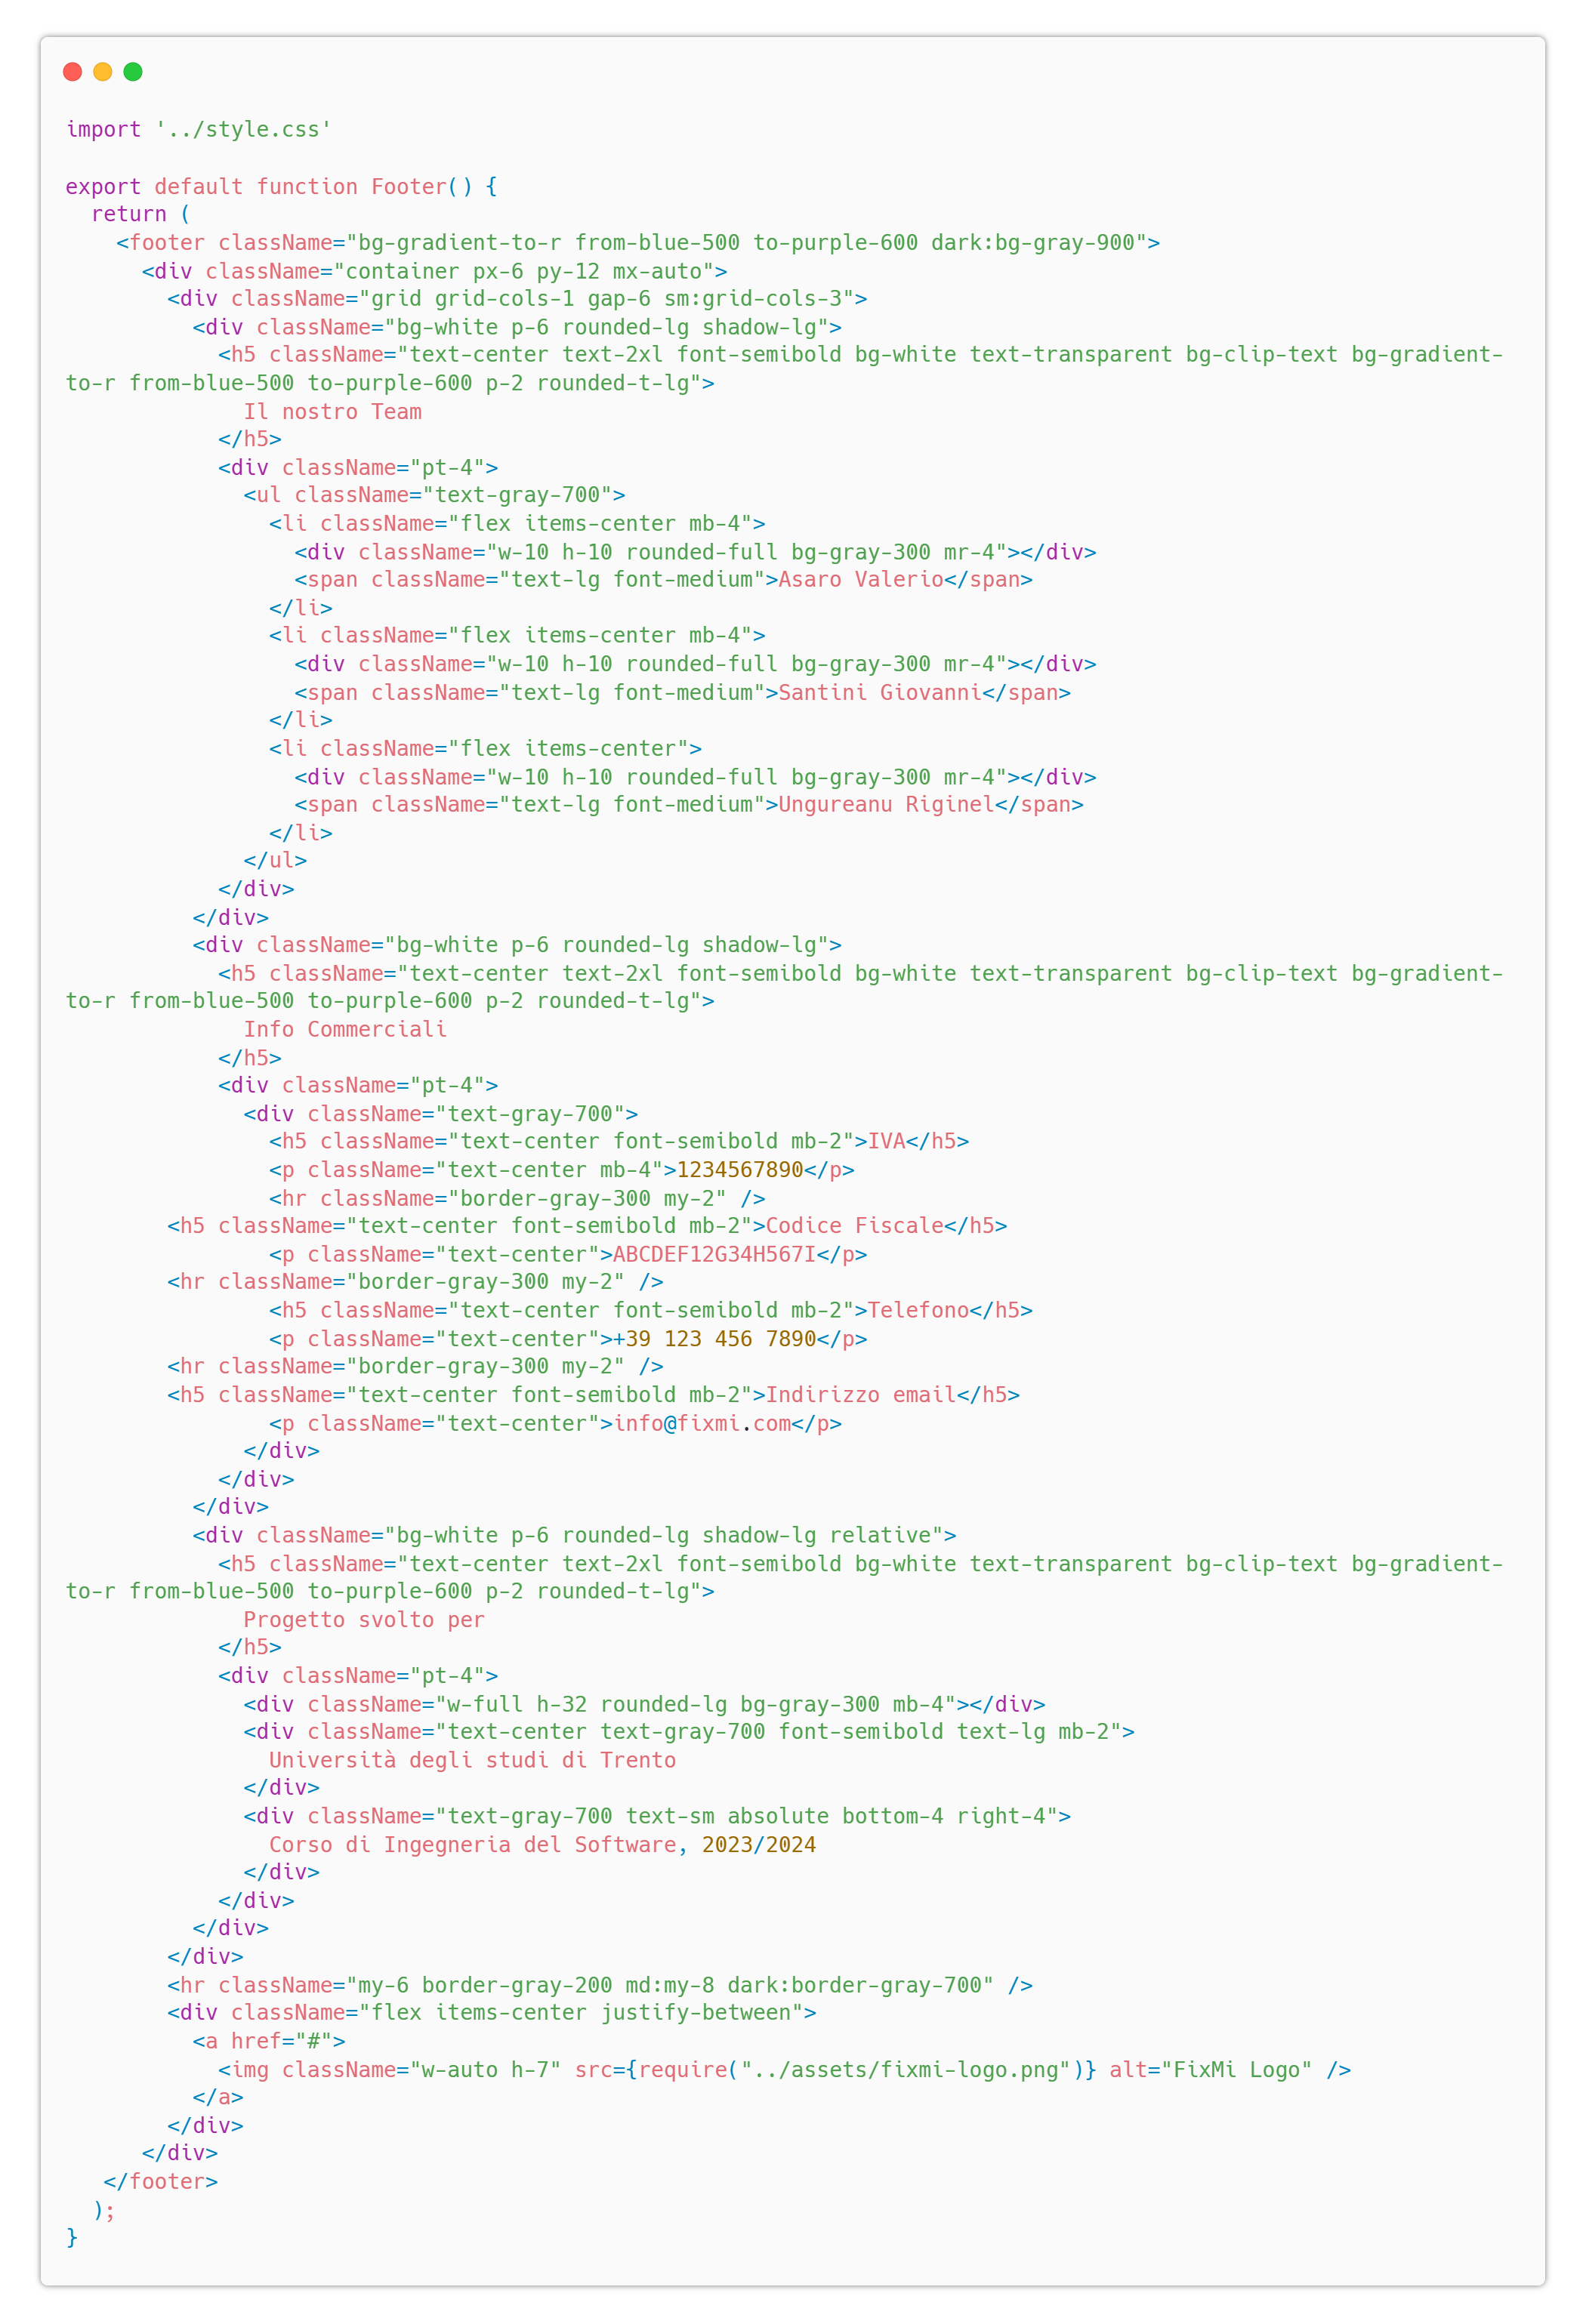
\includegraphics[width=1\textwidth]{images/footer-carbon.png}
	\caption{Codice del componente "footer.tsx"}
\end{figure}

\section{Modellazione dati nel database}
Sono presenti due database MongoDB con i quali i microservizi interagiscono:
\subsection*{Users}
Il database Users contiene i profili dei clienti, dipendenti e manager
\begin{figure}[H]
	\centering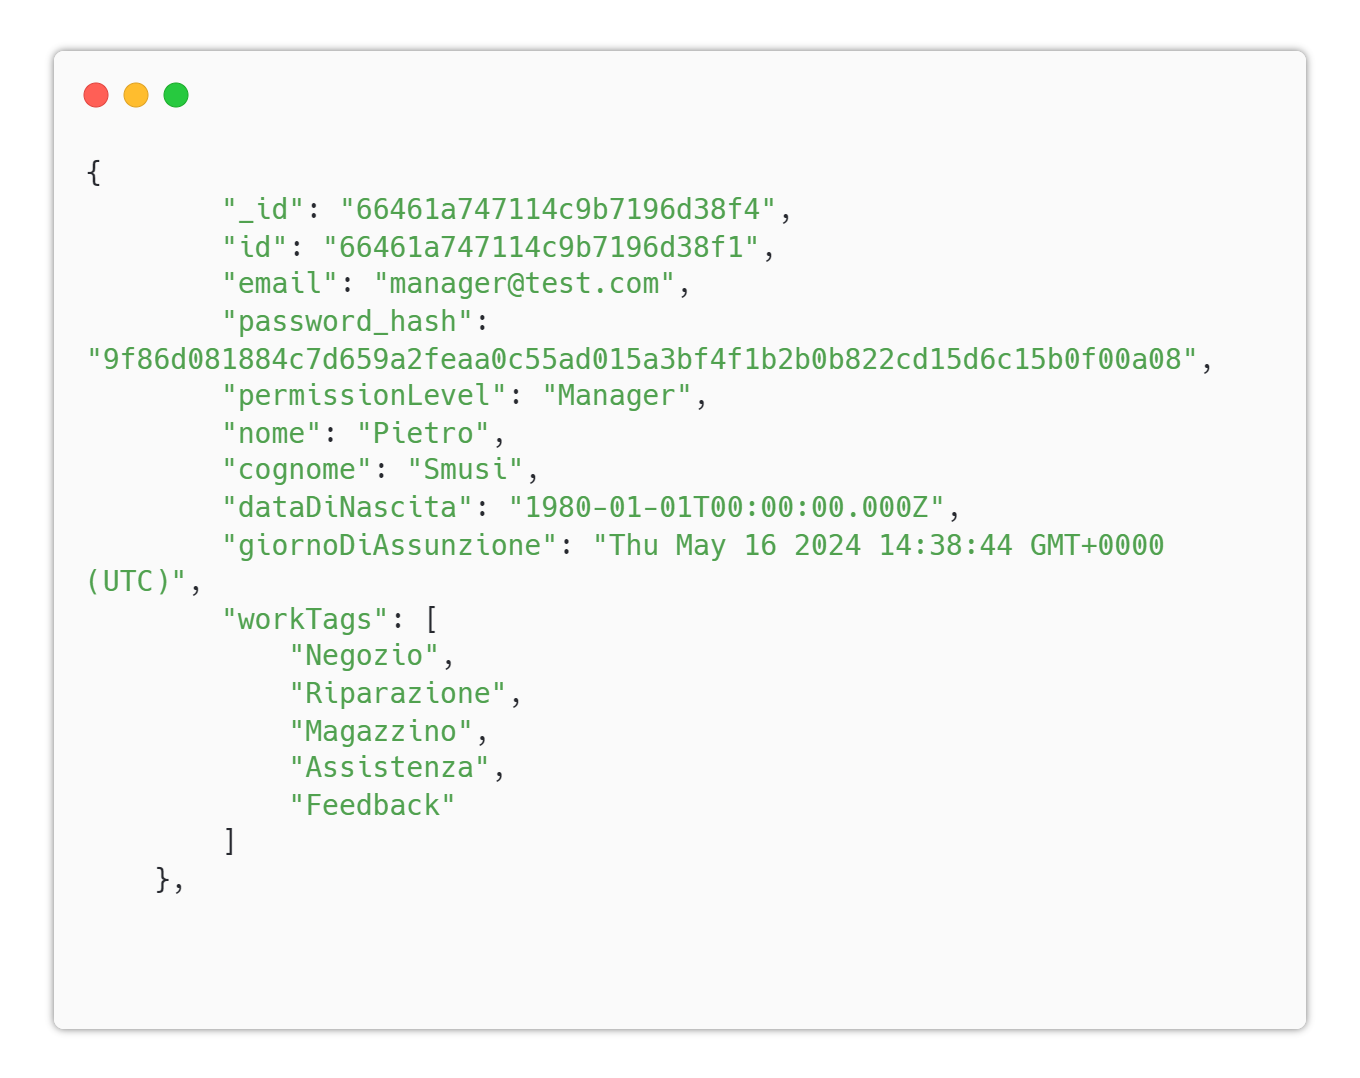
\includegraphics[width=1\textwidth]{images/database/manager.png}
	\caption{Profilo manager nel database}
\end{figure}
\begin{figure}[H]
	\centering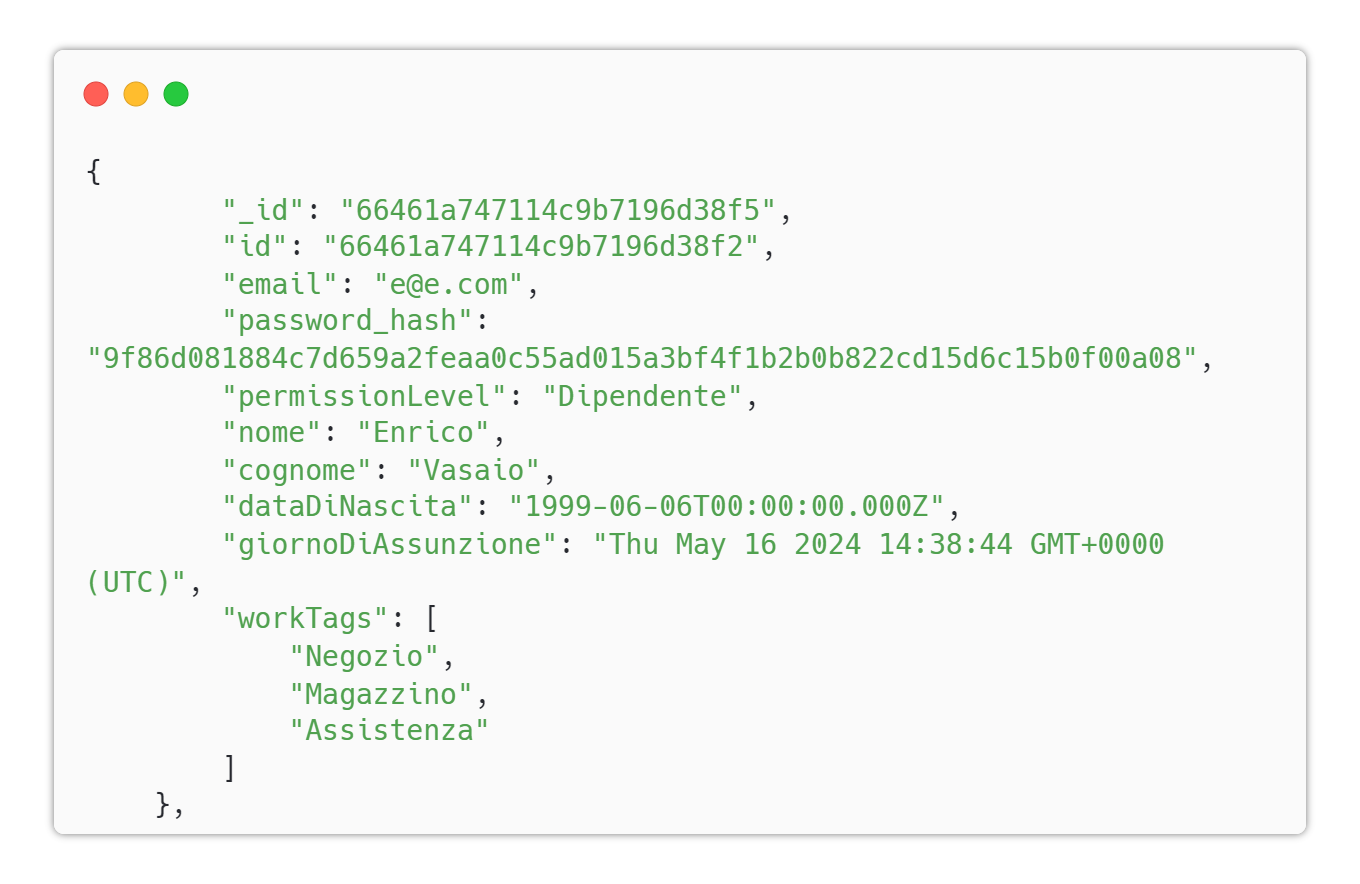
\includegraphics[width=1\textwidth]{images/database/dipendente.png}
	\caption{Profilo dipendente nel database}
\end{figure}
\begin{figure}[H]
	\centering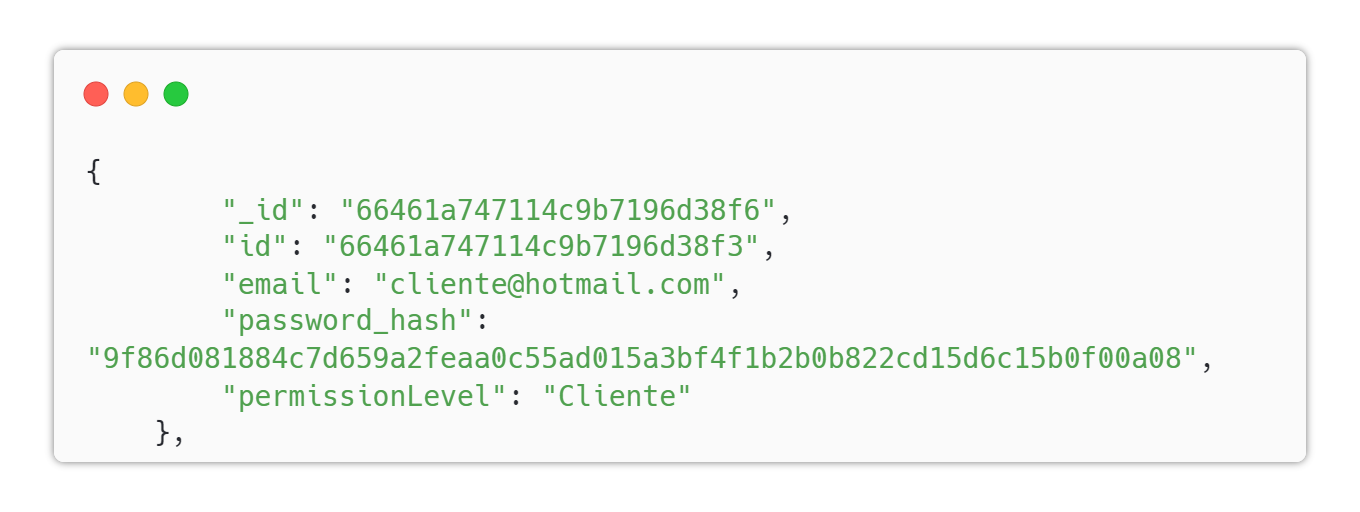
\includegraphics[width=1\textwidth]{images/database/cliente.png}
	\caption{Profilo cliente nel database}
\end{figure}


\subsection*{Tasks}
Il database Tasks contiene le task
\begin{figure}[H]
	\centering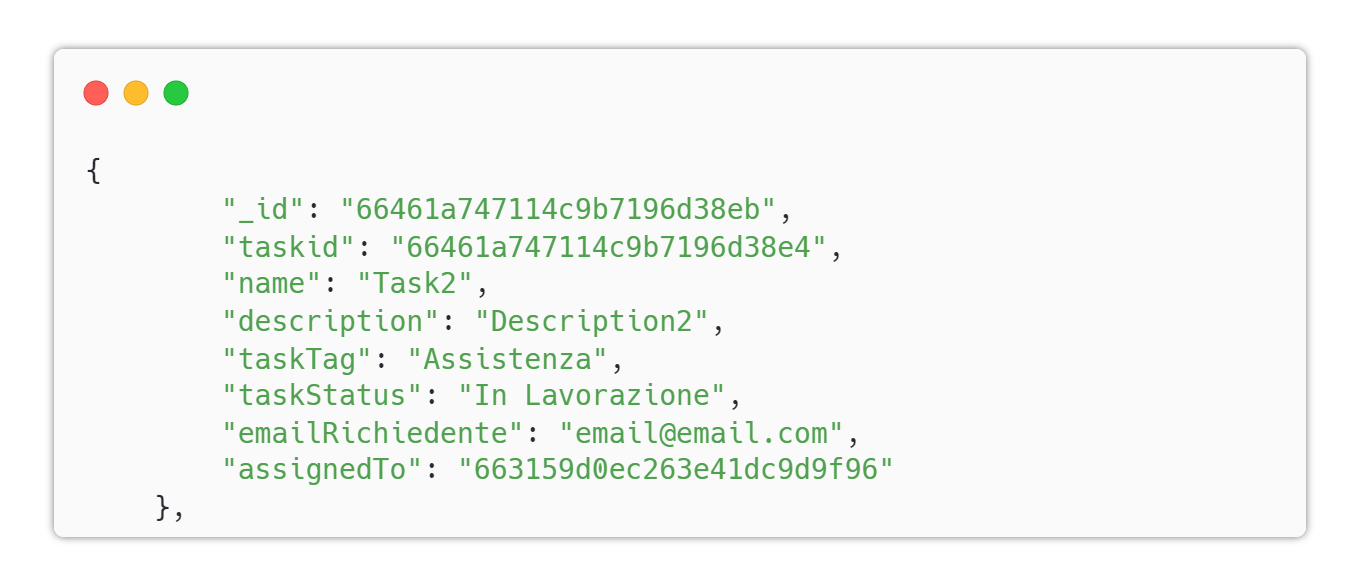
\includegraphics[width=1\textwidth]{images/database/assistenza.png}
	\caption{Task Assistenza nel database}
\end{figure}
\begin{figure}[H]
	\centering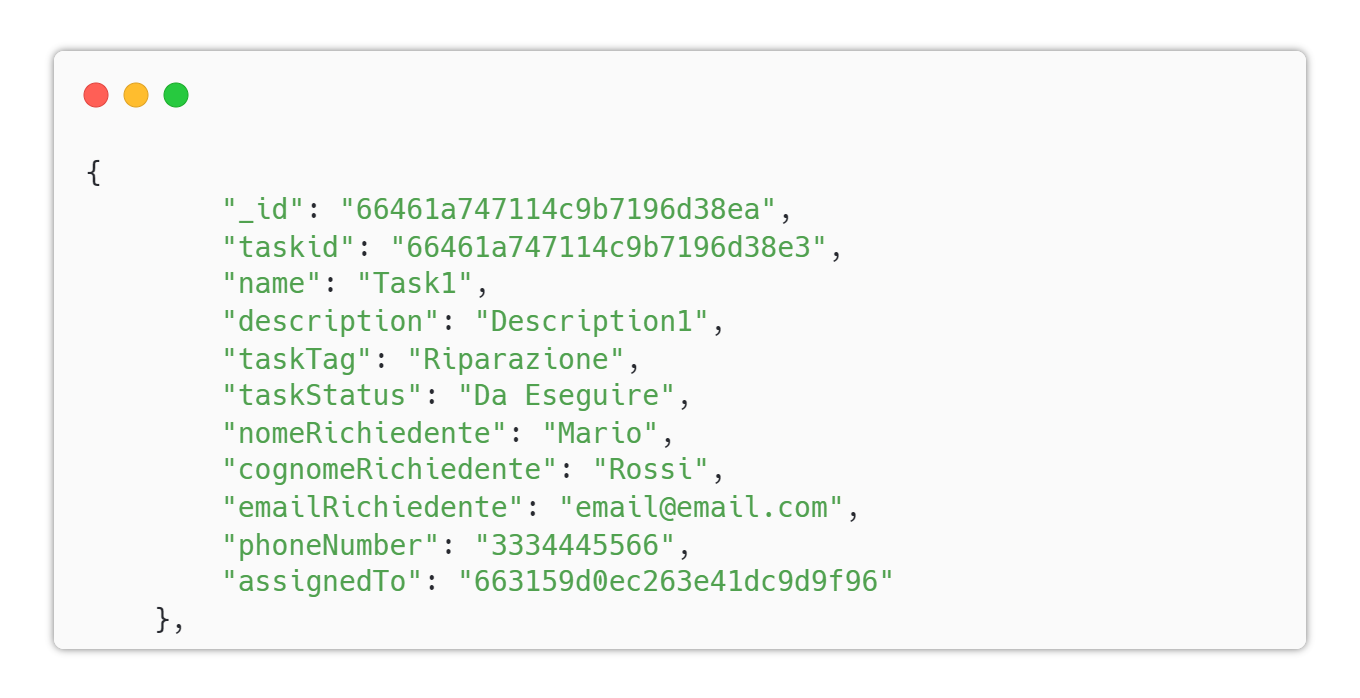
\includegraphics[width=1\textwidth]{images/database/riparazione.png}
	\caption{Task Riparazione nel database}
\end{figure}
\begin{figure}[H]
	\centering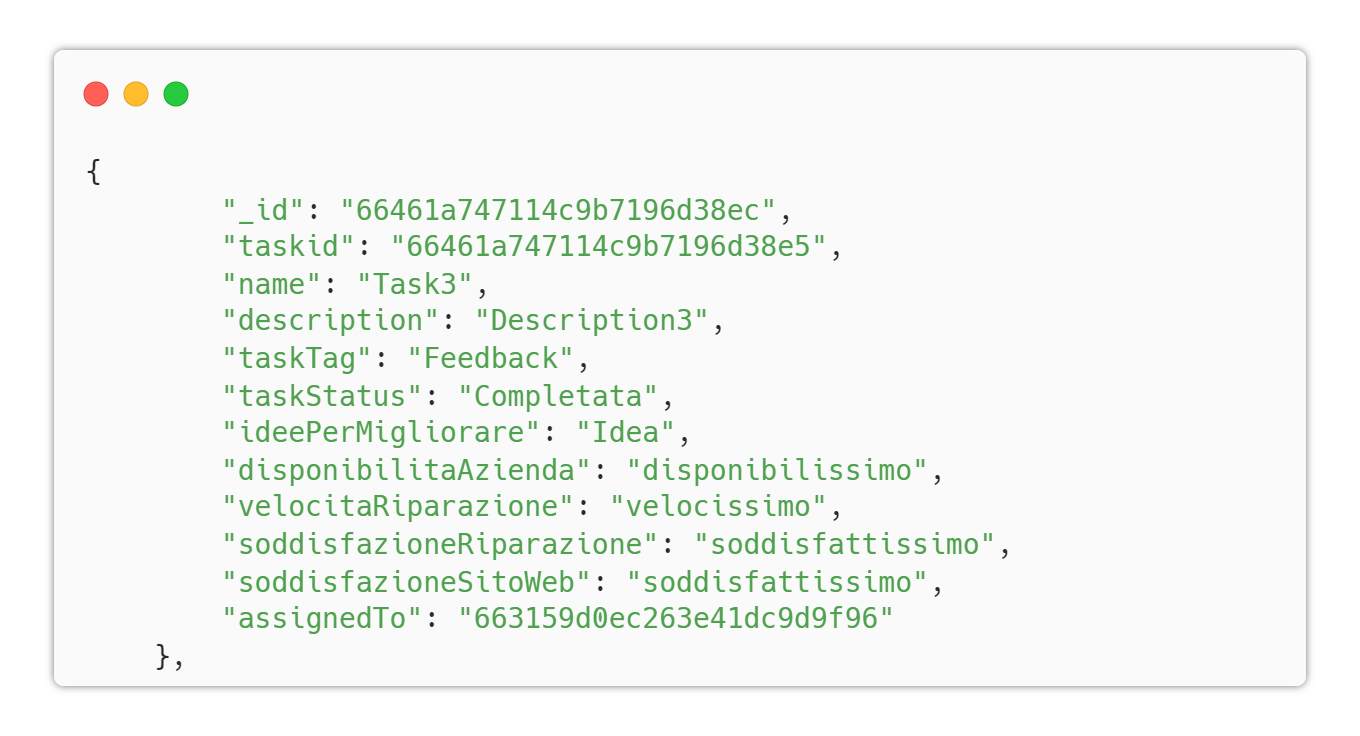
\includegraphics[width=1\textwidth]{images/database/feedback.png}
	\caption{Task Feedback nel database}
\end{figure}
\begin{figure}[H]
	\centering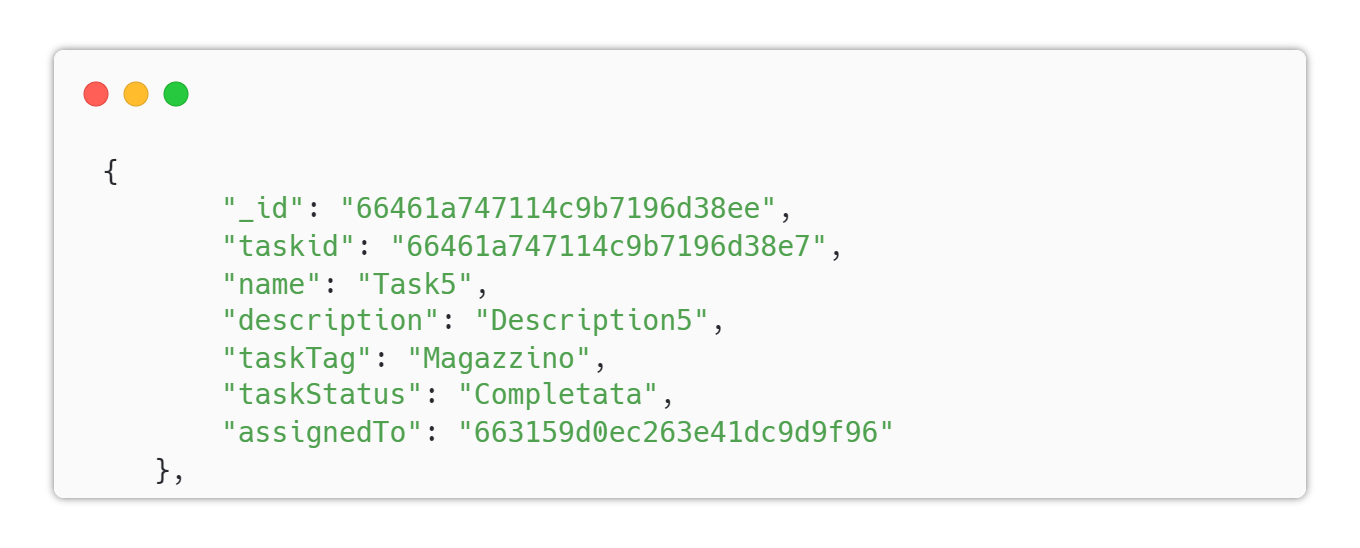
\includegraphics[width=1\textwidth]{images/database/magazzino.png}
	\caption{Task Magazzino nel database}
\end{figure}


\chapter{Microservizio Autenticazione}

\section{Backend}

Questa sezione comprende lo sviluppo e la documentazione del backend del Microservizio Autenticazione

\subsection{Struttura del backend}
La struttura del backend del microservizio autenticazione è riportata
nella figura sotto.
\begin{figure}[H]
	\centering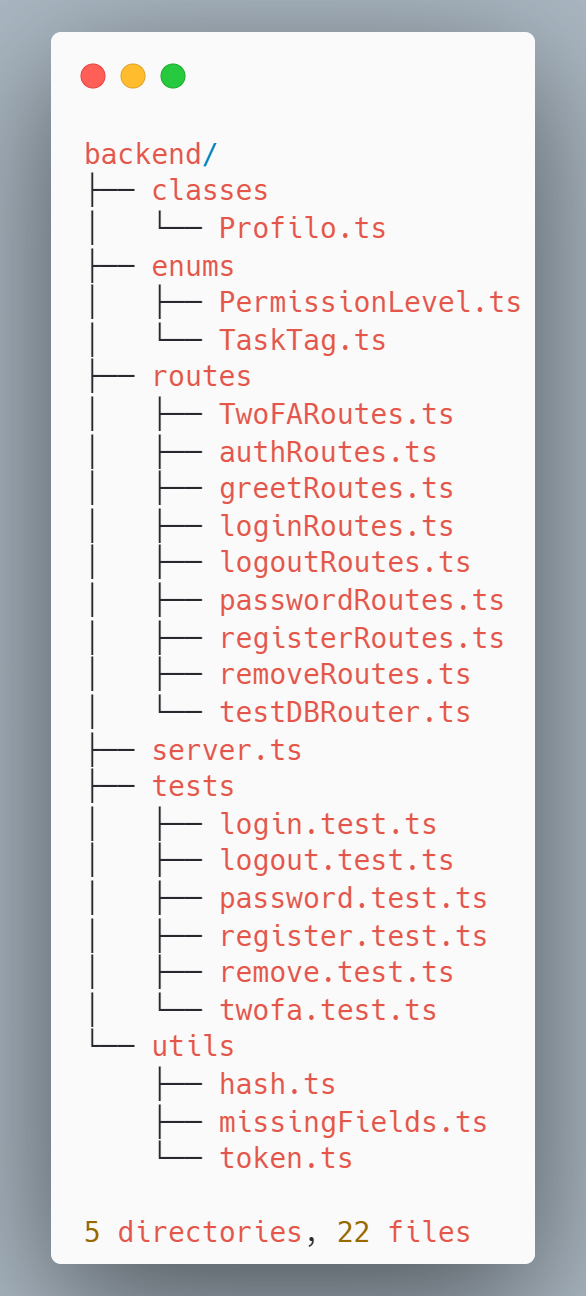
\includegraphics[width=0.5\textwidth]{images/microservizio-autenticazione/backend-structure.png}
	\caption{Output del comando "tree" all'interno di un microservizio.}
\end{figure}





\subsection{Specifica delle risorse}
Di seguito le risorse estratte dal diagramma delle classi e utilizzate da questo microservizio.
\paragraph*{<<resource>> Cliente}
Rappresenta il profilo di un Cliente.
Ha i seguenti attributi
\begin{itemize}
	\item id
	\item email
	\item password\_hash
	\item permissionLevel
	\item token
\end{itemize}
\paragraph*{<<resource>> Dipendente}
Rappresenta il profilo di un Dipendente.
Ha tutti gli attributi di cliente, in più:
\begin{itemize}
	\item nome
	\item cognome
	\item data di assunzione
	\item data di nascita
	\item worktags
\end{itemize}
\paragraph*{Manager}
Rappresenta il profilo del Manager.
Ha tutti gli attributi di Dipendente, ma ha come permissionLevel "Manager"

Metodi
\paragraph*{<<resource>> login}
Permette a un utente già esistente di accedere all'applicazione.
I parametri in ingresso sono email, password e codice 2FA.
E' un'API del backend.

\paragraph*{<<resource>> logout}
Permette a un utente che ha già eseguito l'accesso di svolgere il logout dall'applicazione.
Richiede in ingresso il token di sessione ricevuto al login.

\paragraph*{<<resource>> twofa}
Permette a un utente che vuole eseguire l'accesso, registrarsi per la prima volta, cambiare la password o rimuovere il proprio account di ricevere attraverso email un codice 2FA.
Richiede in ingresso la propria email.

\paragraph*{<<resource>> registrazione}
Permette a un nuovo cliente di registrarsi all'applicazione.
Richiede in ingresso l'email, la password e il codice 2FA

\paragraph*{<<resource>> cambioPassword}
Permette a un utente già esistente  di cambiare la propria password.
Richiede in ingresso l'email, la nuova password e il codice 2FA.

\paragraph*{<<resource>> eliminaProfilo}
Permette a un utente già esistende di eliminare il proprio profilo.
Richiede in ingresso l'email, la password e il codice 2FA.

\paragraph*{<<resource>> autenticaUtente}
Permette a un altro microservizio di autenticare un utente che desidera utilizzare una funzionalità che richiede autorizzazione.
Richiede in ingresso il token dell'utente.

\subsection{Login}
\subsubsection*{Specifica}
Questa API, all'indirizzo /api/auth/login, ha un metodo POST e viene utilizzata per far accedere utenti all'applicazione.
La request body è in formato x-www-form-urlencoded e deve contenere i seguenti campi:
\begin{itemize}
	\item email
	\item password
	\item twofa
\end{itemize}
La response body è in formato application/json. Di seguito le possibili risposte:
% table
\begin{center} % center the table
	\centering
	\begin{tabular}{ |p{4cm}|p{5cm}|p{4cm}| }
		\hline
		\centering Status Code & \qquad\quad Body e Cookie                               & \qquad\qquad Spiegazione                              \\ % I found no other way...
		\hline
		200 OK                 & \{text: "successfully logged in", token\} cookie: token & Login avvenuto con successo                           \\
		\hline
		400 BAD REQUEST        & \{error: "missing fields", missingFields\}              & Alcuni campi non sono stati specificati nella request \\ % I found no other way...
		\hline
		404 NOT FOUND          & \{error: "user not found"\}                             & non esiste utente con la mail fornita                 \\% I found no other way...
		\hline
		404 NOT FOUND          & \{error: "wrong password" \}                            & la password inserita non è corretta                   \\
		\hline
		400 BAD REQUEST        & \{error: "2fa not correct" \}                           & Il codice twofa inserito non è corretto.              \\
		\hline
	\end{tabular}
\end{center}
\begin{figure}[H]
	\centering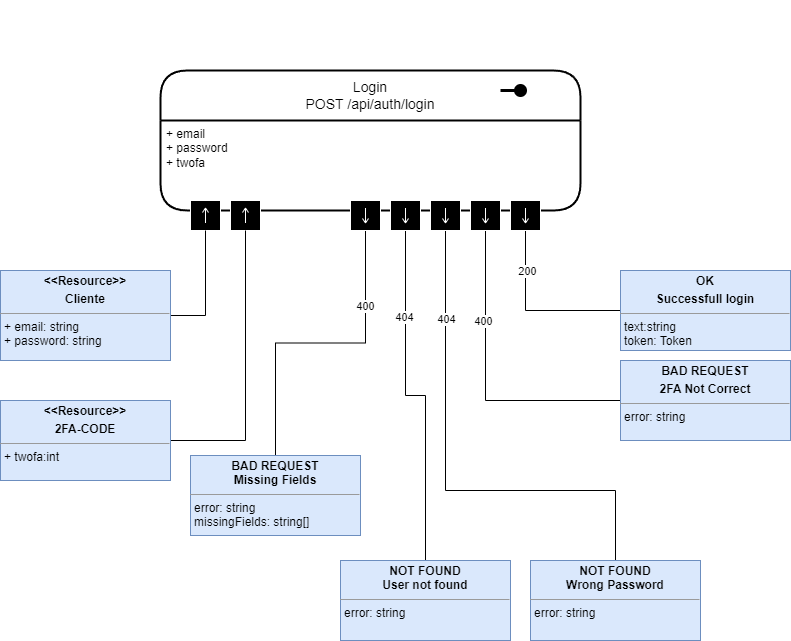
\includegraphics[width=1\textwidth]{images/microservizio-autenticazione/diagrams/diagramma_login.drawio.png}
	\caption{Diagramma dell'endpoint "login"}
\end{figure}

\subsubsection*{Specifica OpenAPI}
Di seguito la specifica openapi dell'endpoint login contenuta nel file 'openapi.yaml' della directory del microservizio
\begin{verbatim}
	/login:
    post:
      summary: Login method for user authentication
      description: This endpoint allows users to log in by providing email, password, and two-factor authentication code.
      requestBody:
        required: true
        content:
          application/x-www-form-urlencoded:
            schema:
              type: object
              properties:
                email:
                  type: string
                  format: email

                password:
                  type: string
                  format: password
                  
                twofa:
                  type: string
                  format: twofa-code
               
              required:
                - email
                - password
                - twofa
      responses:
        '200':
          description: Successfully logged in
          content:
            application/json:
              schema:
                type: object
                properties:
                  text:
                    type: string
                    example: "successfully logged in!"
                  token:
                    type: string
                    example: "12415343463452"
            

          headers:
            Set-Cookie:
              schema:
                type: string
              description: Session token
        '400':
          description: Bad Request - Missing fields or 2fa not correct
          content:
            application/json:
              schema:
                oneOf:
                  - $ref: '#/components/schemas/missingFieldsSchema'
                  - $ref: '#/components/schemas/wrongTwoFaSchema'
      
        '404':
          description: User not found or wrong password
          content:
            application/json:
              schema:
                oneOf:
                  - $ref: '#/components/schemas/notFoundSchema'
                  - $ref: '#/components/schemas/wrongPassSchema'
\end{verbatim}

\subsubsection*{Codice}
Questa API viene utilizzata da un utente per eseguire l'accesso.
Una volta ricevuta la richiesta, viene controllata la presenza di tutti i campi richiesti.
Successivamente si controlla se l'utente esista o meno nel database, e successivamente la validità della password.
Dopo aver controllato che il codice 2FA sia corretto, viene generato un token, aggiunto alla sessione e inviato sia nel body sia come cookie nella risposta.


\begin{figure}[H]
	\centering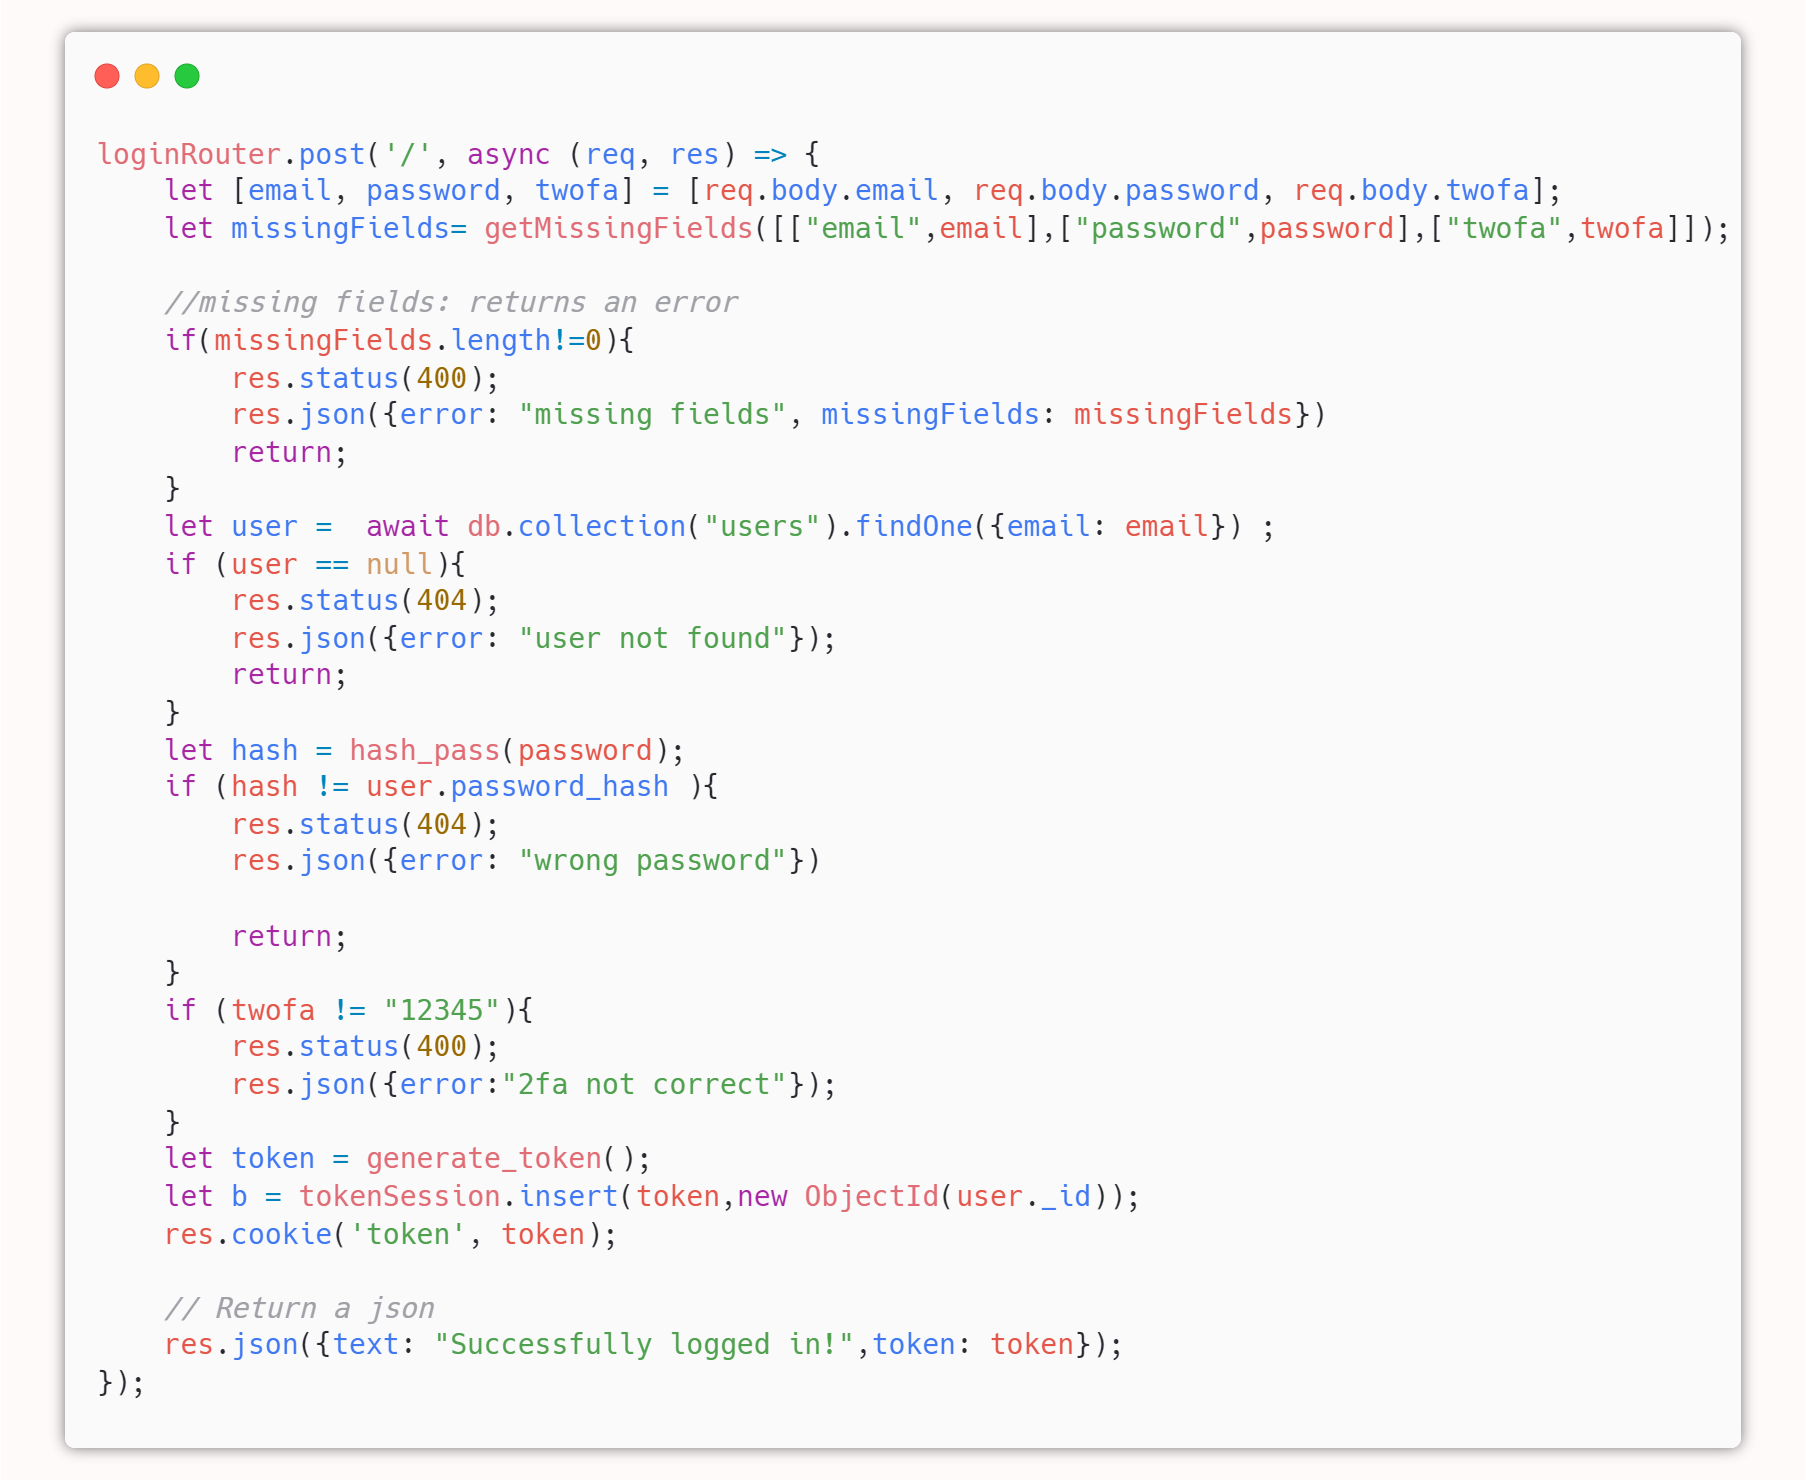
\includegraphics[width=1\textwidth]{images/microservizio-autenticazione/login-carbon.png}
	Codice dell'API api/auth/login
\end{figure}

\subsubsection*{Testing}
Per questo endpoint sono stati creati i seguenti test:
\begin{center} % center the table
	\centering
	\begin{tabular}{ |p{1cm}|p{2cm}|p{2cm}|p{2cm}|p{2cm}|p{1cm}|p{1cm}| }
		\hline
		Numero Testcase & Descrizione Test Case & Test Data                   & Precondizioni                                          & Dipendenze & Res Atteso & Res Riscontrato \\
		\hline
		1               & Login con successo    & \{email, password, twofa\}  & email e pass già esistenti nel sistema, twofa corretto & DB         & 200        & 200             \\
		\hline
		2               & Mancanza campi        & \{ \}                       &                                                        &            & 400        & 400             \\
		\hline
		3               & Utente non esiste     & \{ email, password, twofa\} & L'account non esiste                                   & DB         & 404        & 404             \\
		\hline
		4               & Password non valida   & \{ email,password,twofa\}   & email già esistente nel sistema                        & DB         & 404        & 404             \\
		\hline
	\end{tabular}
\end{center}
\begin{figure}[H]
	\centering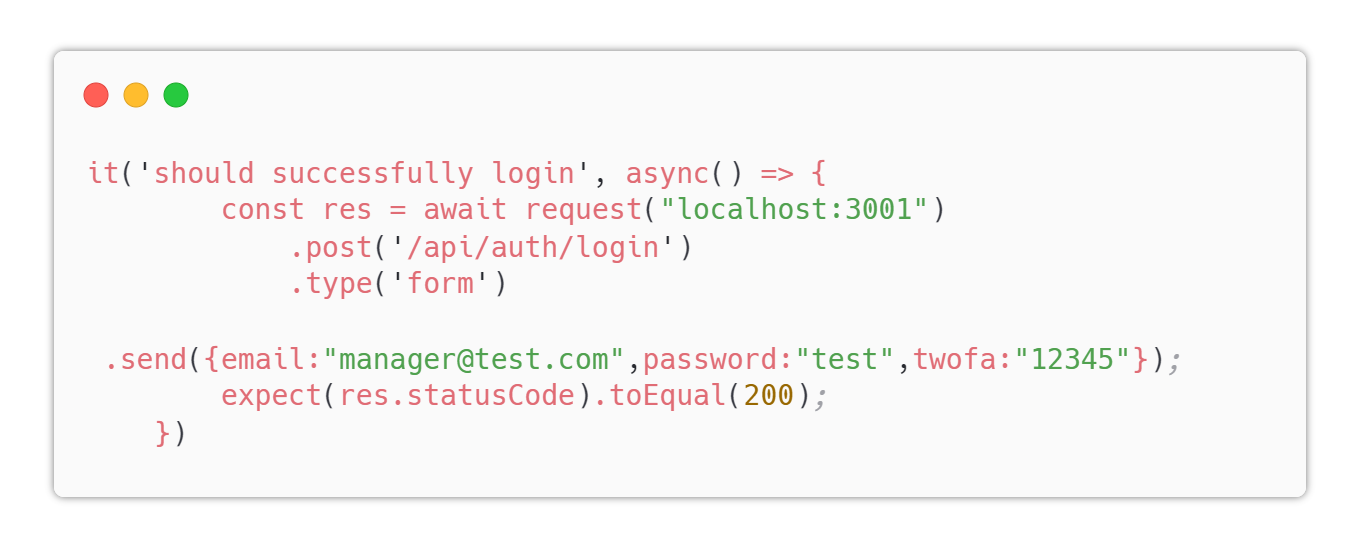
\includegraphics[width=1\textwidth]{images/microservizio-autenticazione/tests/login_test_1.png}
	\caption{Test Login 1}
\end{figure}
\begin{figure}[H]
	\centering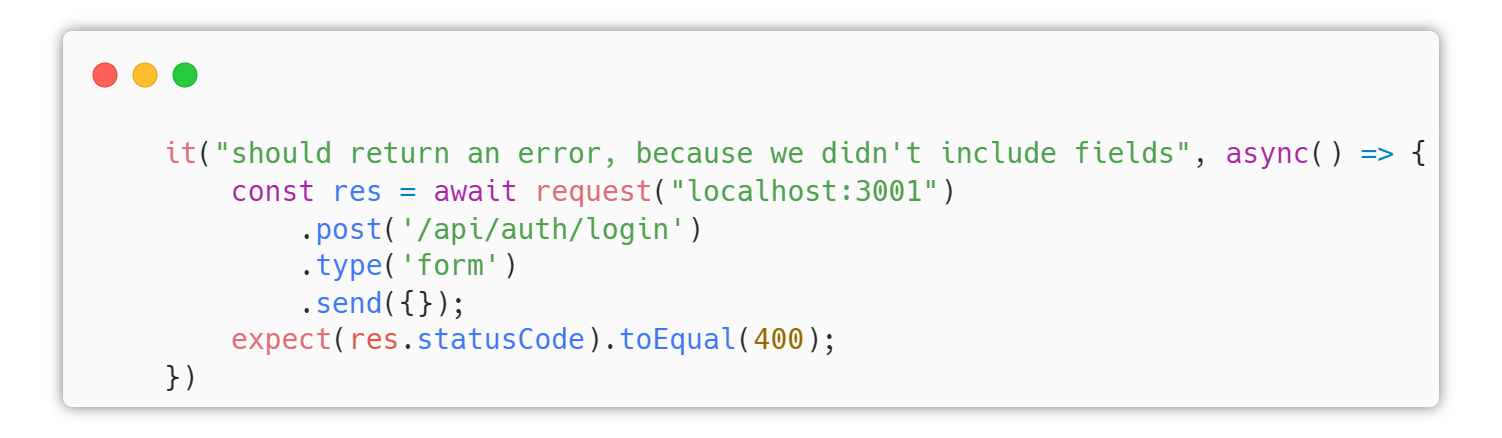
\includegraphics[width=1\textwidth]{images/microservizio-autenticazione/tests/login_test_2.png}
	\caption{Test Login 2}
\end{figure}
\begin{figure}[H]
	\centering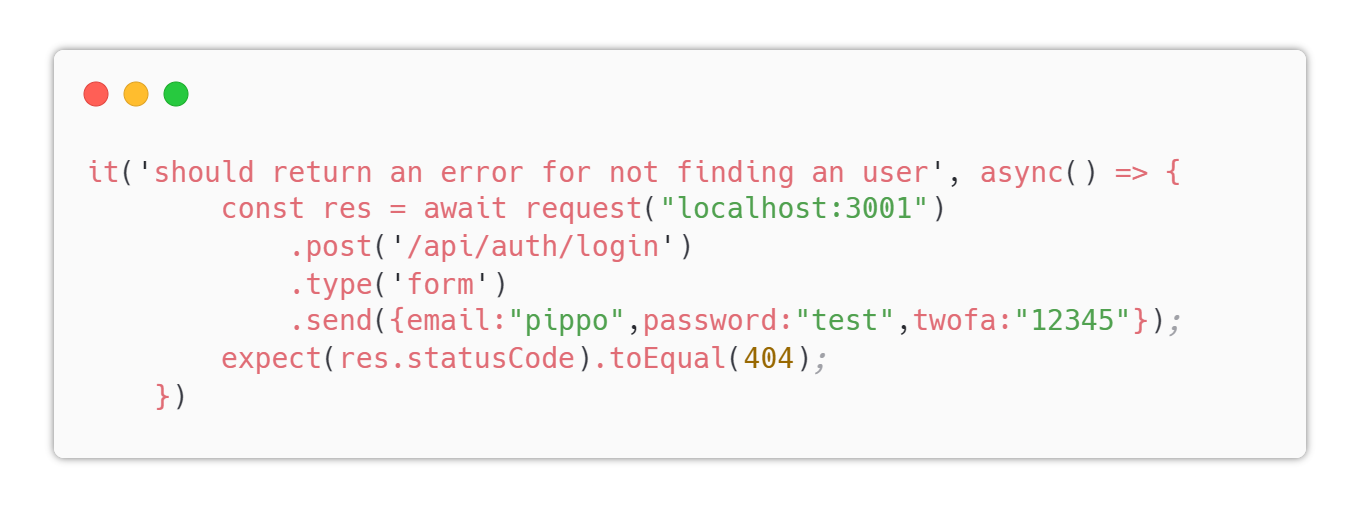
\includegraphics[width=1\textwidth]{images/microservizio-autenticazione/tests/login_test_3.png}
	\caption{Test Login 3}
\end{figure}
\begin{figure}[H]
	\centering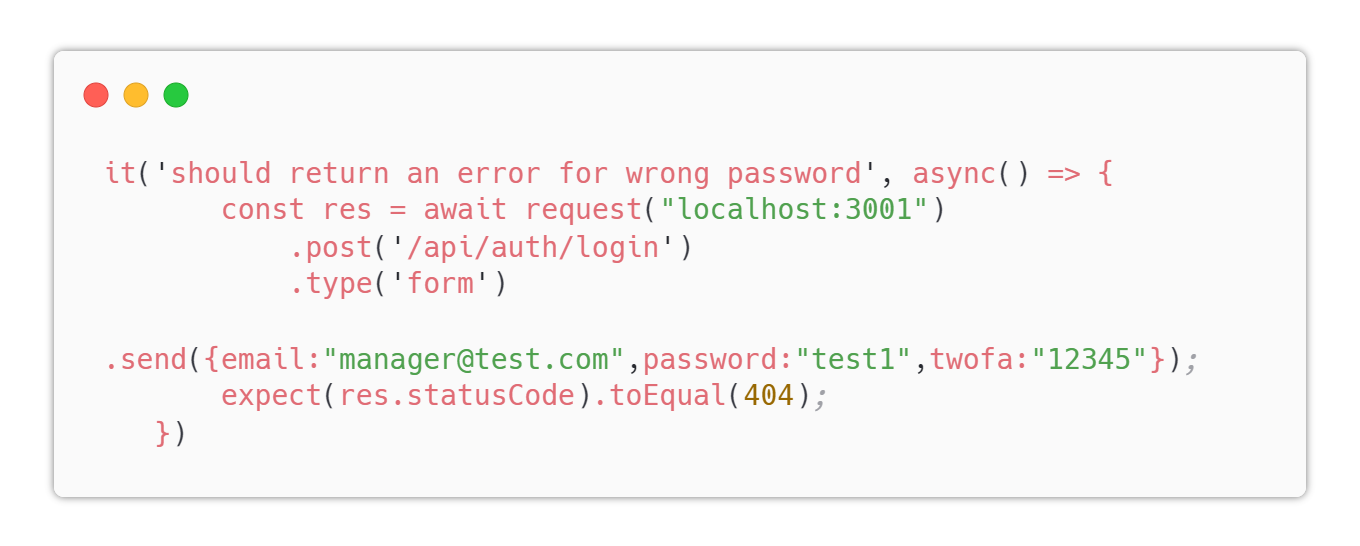
\includegraphics[width=1\textwidth]{images/microservizio-autenticazione/tests/login_test_4.png}
	\caption{Test Login 4}
\end{figure}
I risultati dei test sono i seguenti:
\begin{figure}[H]
	\centering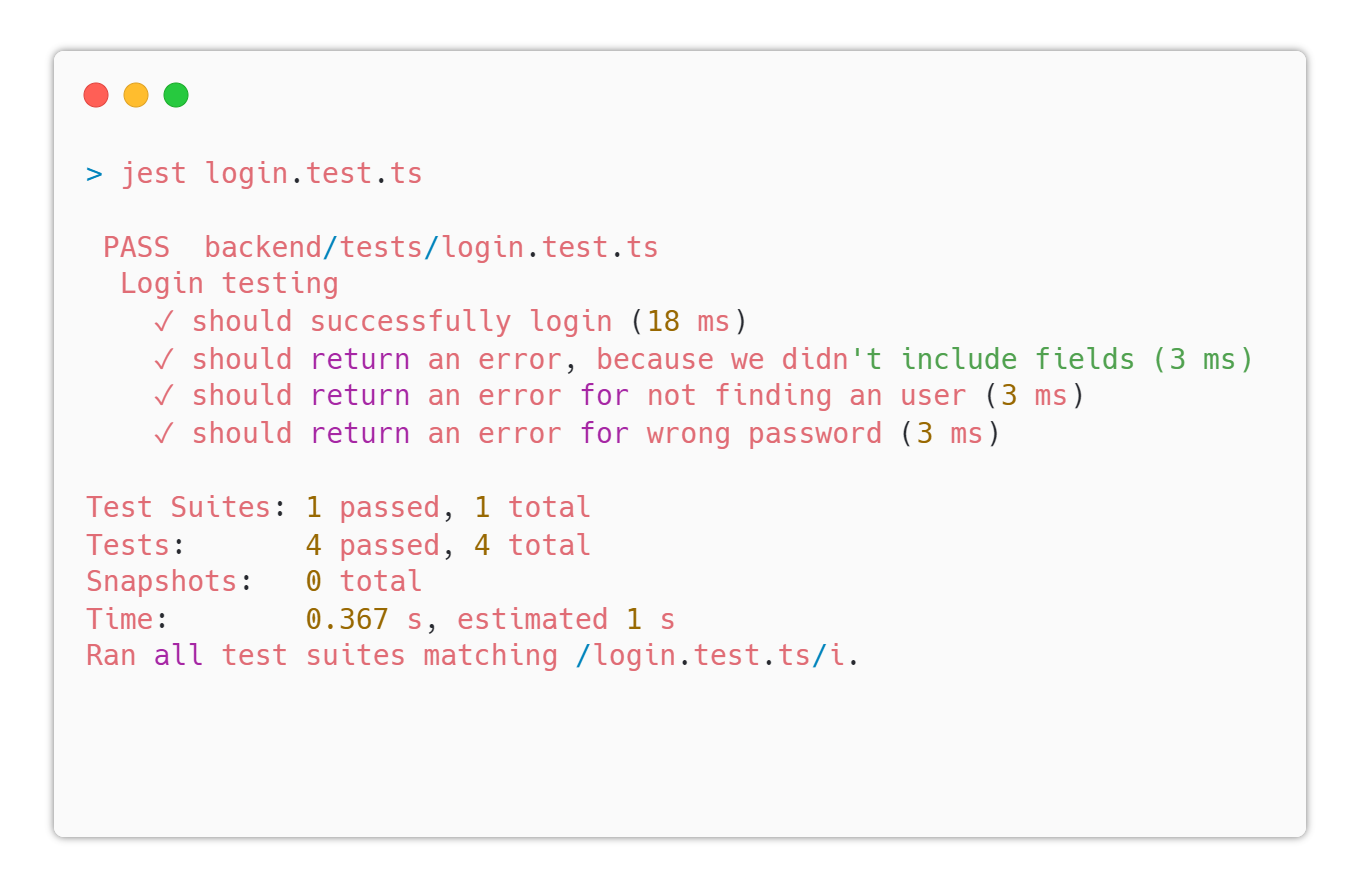
\includegraphics[width=1\textwidth]{images/microservizio-autenticazione/tests/login_test_results.png}
	\caption{Risultati test}
\end{figure}
\subsection{Logout}
\subsubsection*{Specifica}


Questa API, all'indirizzo/api/auth/logout, ha un metodo DELETE e viene utilizzata da un utente autenticato per svolgere il logout.
La request body è in formato x-www-form-urlencoded e deve contenere il token dell'utente.
La response body è in formato application/json. di seguito le possibili risposte:
% table
\begin{center} % center the table
	\centering
	\begin{tabular}{ |p{4cm}|p{5cm}|p{4cm}| }
		\hline
		\centering Status Code & \qquad\quad Body e Cookie                        & \qquad\qquad Spiegazione                               \\ % I found no other way...
		\hline
		200 OK                 & \{text: "successfully logged out"\}              & Logout avvenuto con successo                           \\
		\hline
		400 BAD REQUEST        & \{error: "missing fields", missingFields\}       & Alcuni campi non sono stati specificati nella request  \\ % I found no other way...
		\hline
		404 NOT FOUND          & \{error: "user not found with the given token"\} & non esiste utente nella sessione con il token fornito. \\% I found no other way...
		\hline
		404 NOT FOUND          & \{error: "wrong password" \}                     & la password inserita non è corretta                    \\
		\hline
	\end{tabular}
\end{center}
\begin{figure}[H]
	\centering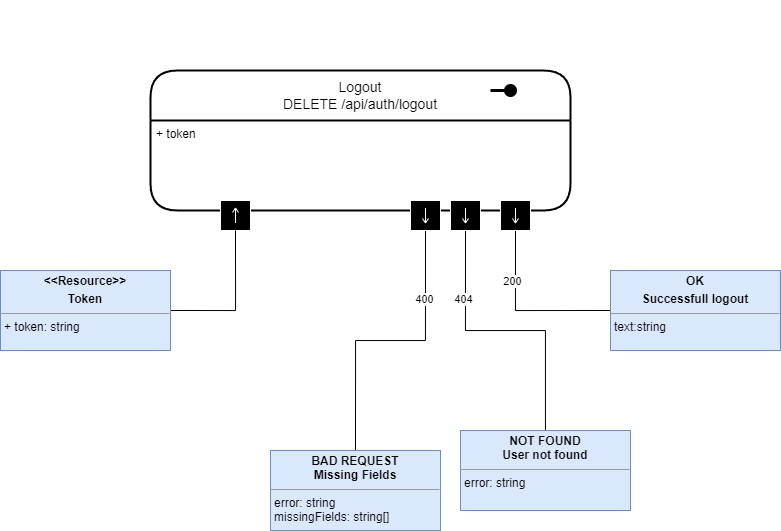
\includegraphics[width=1\textwidth]{images/microservizio-autenticazione/diagrams/diagramma_logout.drawio.png}
	\caption{Diagramma dell'endpoint "logout"}
\end{figure}


\subsubsection*{Specifica OpenAPI}
Di seguito la specifica openapi dell'endpoint logout contenuta nel file 'openapi.yaml' della directory del microservizio
\begin{verbatim}
	/logout:
    delete:
      summary: Method for logging out 
      description: This endpoint allows users who have already logged in to log out by providing their token.
      requestBody:
        required: true
        content:
          application/x-www-form-urlencoded:
            schema:
              type: object
              properties:
                token:
                  type: string
              required:
                  - token
      responses:
        '200':
          description: Succesfully logged out
          content:
            application/json:
              schema:
                type: object
                properties:
                  text:
                    type: string
                    example: "Succesfully logged out!"
        '400':
          description: Bad Request - Missing fields 
          content:
            application/json:
              schema:
                $ref: '#/components/schemas/missingFieldsSchema'
        '404':
          description: User not found with the given token
          content:
            application/json:
              schema:
                $ref: '#/components/schemas/notFoundSchema'
	
\end{verbatim}

\subsubsection*{Codice}
Questa API viene utilizzata da un utente già autenticato per eseguire il logout.
Una volta ricevuta la richiesta, viene controllata la presenza di tutti i campi richiesti.
Successivamente si controlla se il token fornito è presente nella sessione.
A operazione completata, viene rimosso il token dalla sessione.


\begin{figure}[H]
	\centering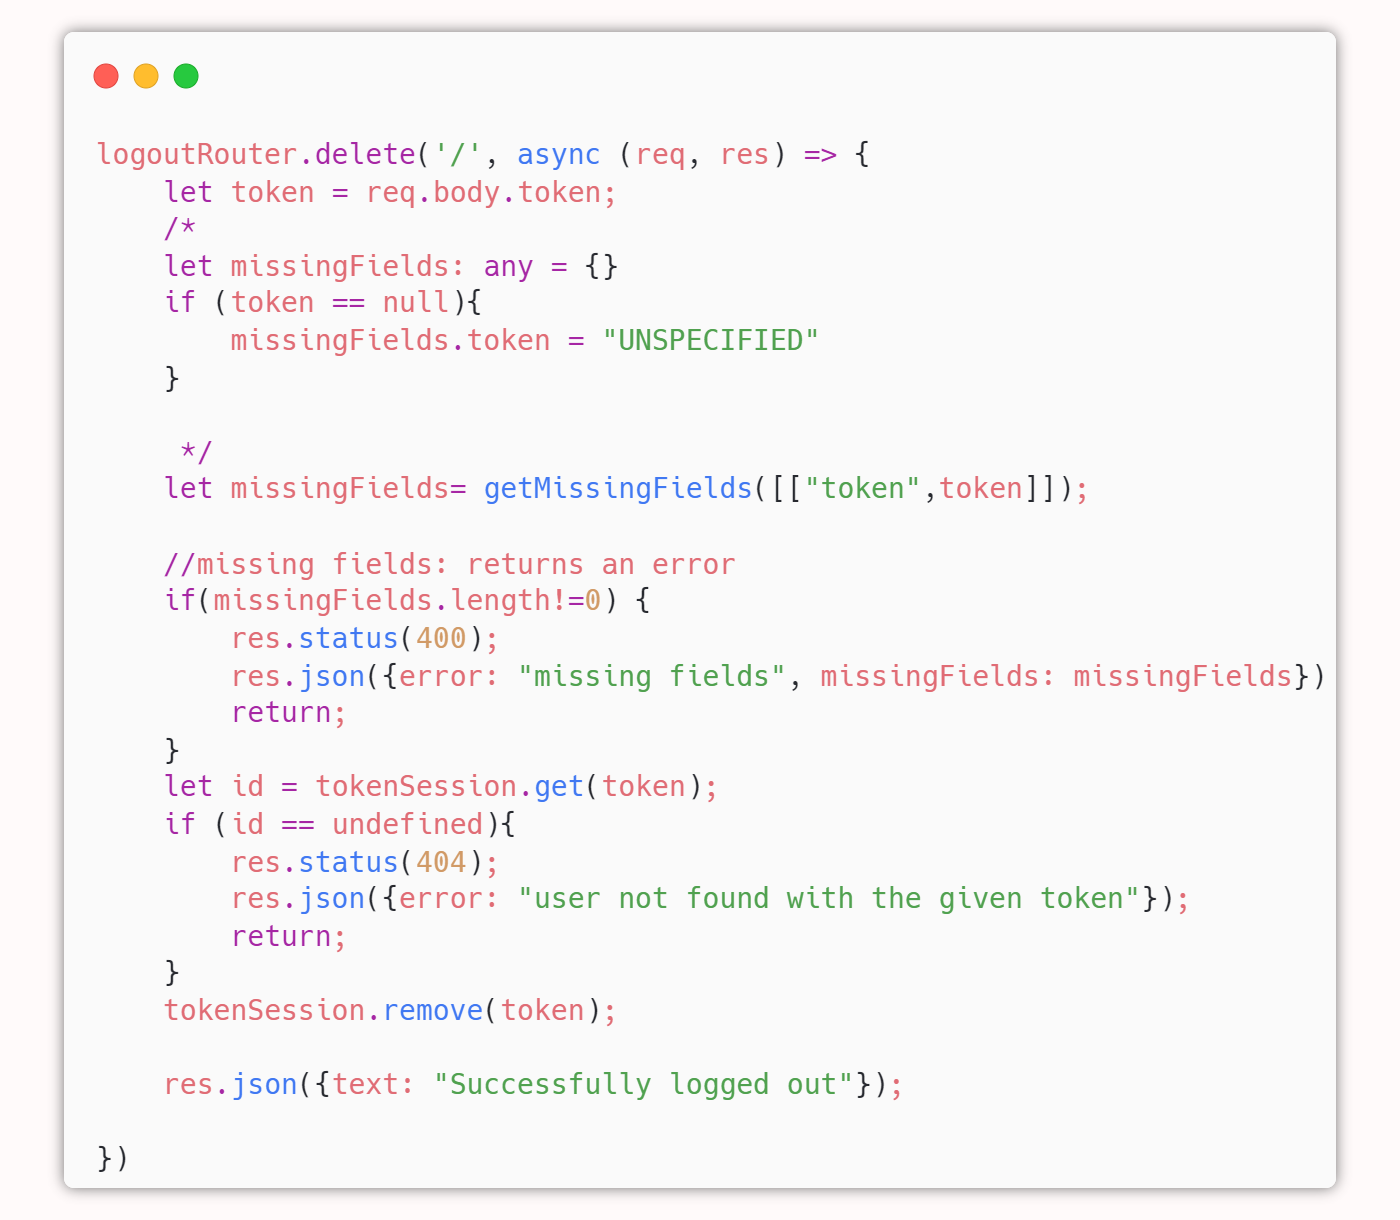
\includegraphics[width=1\textwidth]{images/microservizio-autenticazione/logout-carbon.png}
	Codice dell'API api/auth/logout
\end{figure}


\subsubsection*{Testing}
Per questo endpoint sono stati creati i seguenti test:

\begin{center} % center the table
	\centering
	\begin{tabular}{ |p{1cm}|p{2cm}|p{2cm}|p{2cm}|p{2cm}|p{1cm}|p{1cm}| }
		\hline
		Numero Testcase & Descrizione Test Case            & Test Data  & Precondizioni                     & Dipendenze & Res Atteso & Res Riscontrato \\
		\hline
		1               & Logout con successo              & \{token\}  & Token ottenuto dal login          &            & 200        & 200             \\
		\hline
		2               & Mancanza campi                   & \{ \}      &                                   &            & 400        & 400             \\
		\hline
		3               & Token non presente nella session & \{ token\} & Token non presente nella sessione &            & 404        & 404             \\
		\hline
	\end{tabular}
\end{center}
\begin{figure}[H]
	\centering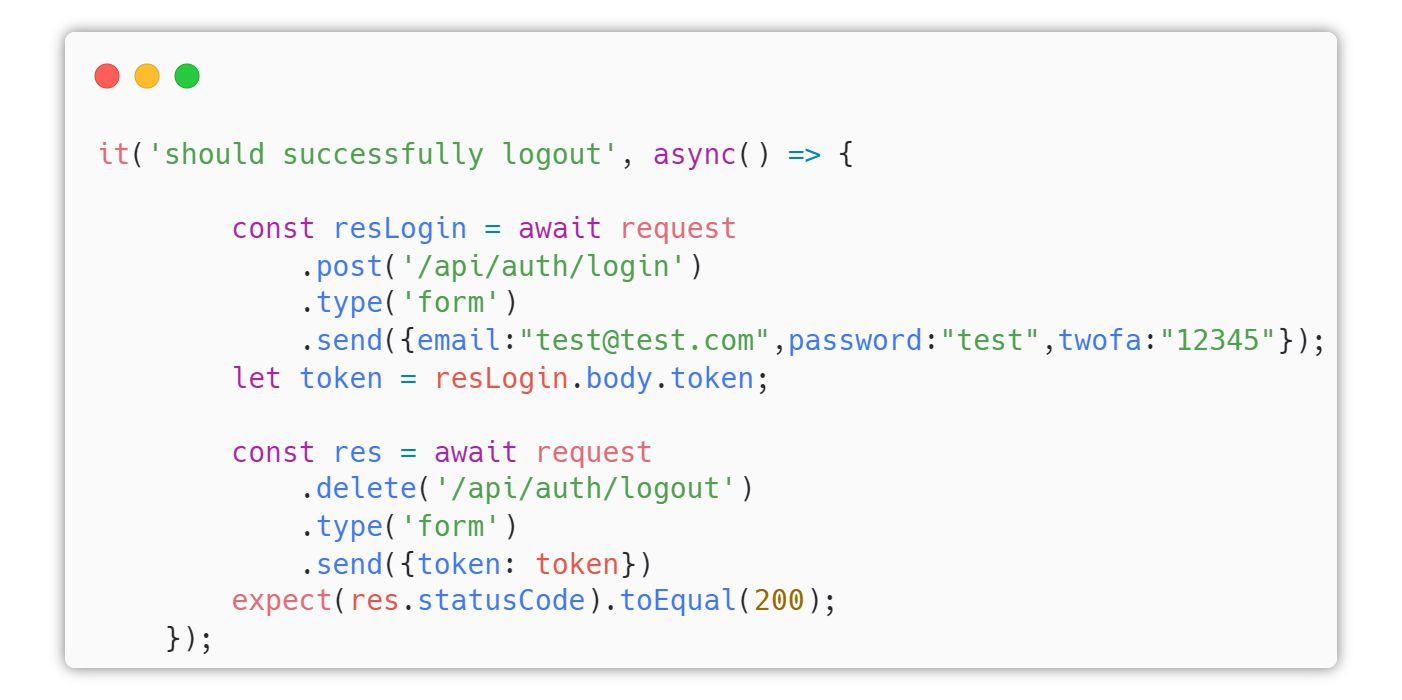
\includegraphics[width=1\textwidth]{images/microservizio-autenticazione/tests/logout_test_1.png}
	\caption{Test Logout 1}
\end{figure}
\begin{figure}[H]
	\centering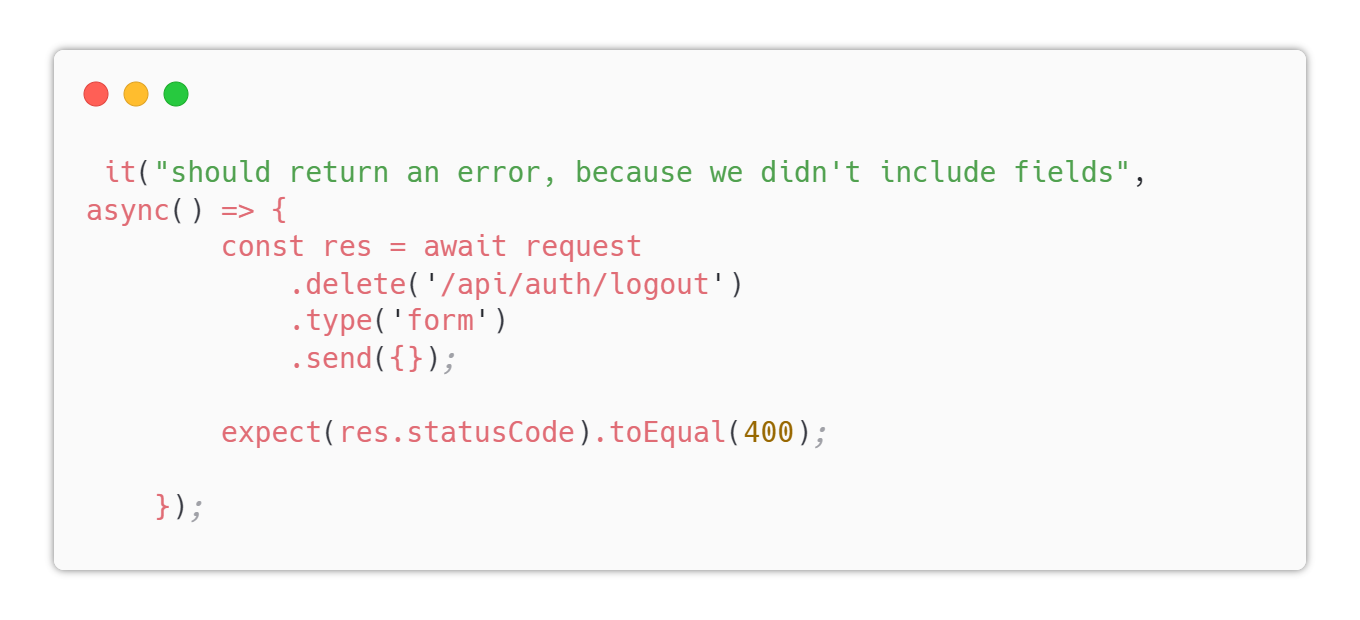
\includegraphics[width=1\textwidth]{images/microservizio-autenticazione/tests/logout_test_2.png}
	\caption{Test Logout 2}
\end{figure}
\begin{figure}[H]
	\centering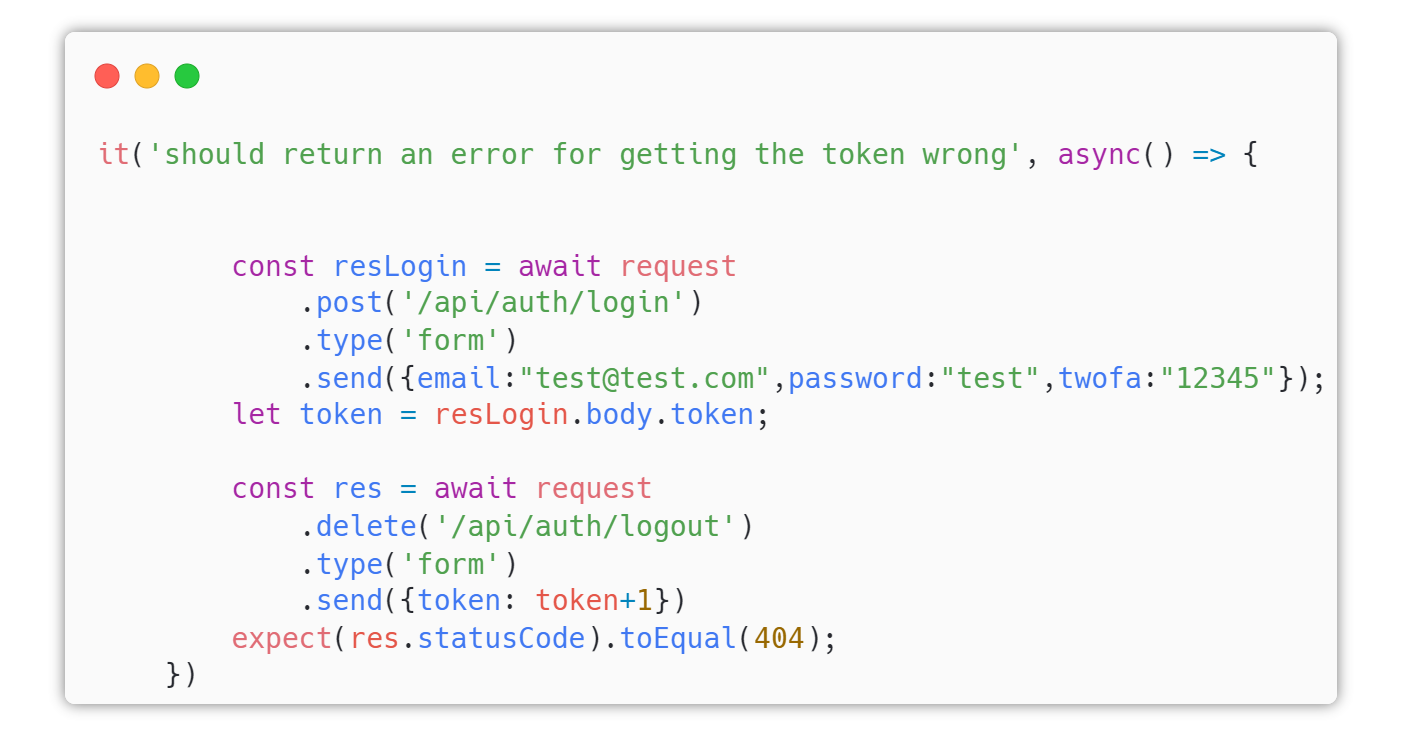
\includegraphics[width=1\textwidth]{images/microservizio-autenticazione/tests/logout_test_3.png}
	\caption{Test Logout 3}
\end{figure}
I risultati dei test sono i seguenti:
\begin{figure}[H]
	\centering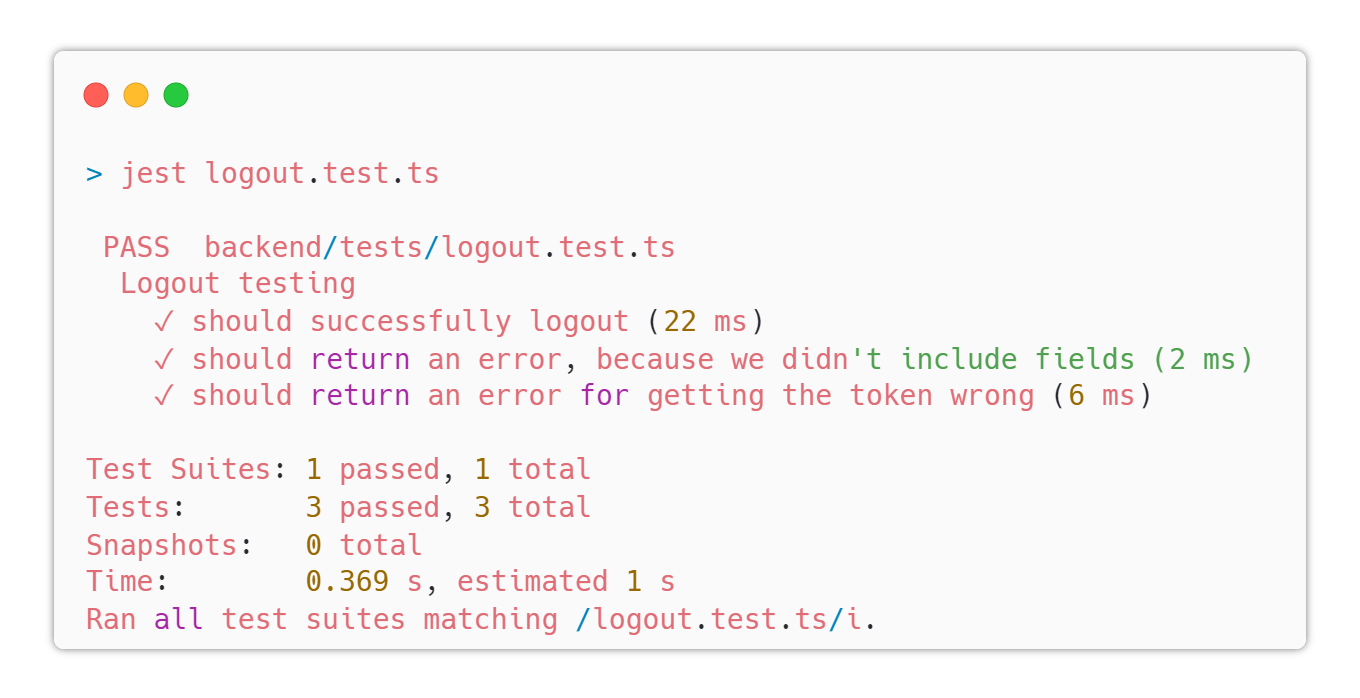
\includegraphics[width=1\textwidth]{images/microservizio-autenticazione/tests/logout_test_results.png}
	\caption{Risultati test}
\end{figure}
\subsection{Registrazione}
\subsubsection*{Specifica}
Questa API, all'indirizzo /api/auth/register, ha un metodo POST e viene utilizzata per la creazione di un account cliente.
La request body è in formato x-www-form-urlencoded e deve contenere i seguenti campi:
\begin{itemize}
	\item email
	\item password
	\item twofa
\end{itemize}
La response body è in formato application/json. Di seguito le possibili risposte:
% table
\begin{center} % center the table
	\centering
	\begin{tabular}{ |p{4cm}|p{5cm}|p{4cm}| }
		\hline
		\centering Status Code & \qquad\quad Body e Cookie                                & \qquad\qquad Spiegazione                              \\ % I found no other way...
		\hline
		200 OK                 & \{text: "successfully registered", token\} cookie: token & Login avvenuto con successo                           \\
		\hline
		400 BAD REQUEST        & \{error: "missing fields", missingFields\}               & Alcuni campi non sono stati specificati nella request \\ % I found no other way...
		\hline
		404 NOT FOUND          & \{error: "user already exists with the given email"\}    & Esiste già un utente con la mail fornita              \\% I found no other way...
		\hline
		400 BAD REQUEST        & \{error: "2fa not correct" \}                            & Il codice twofa inserito non è corretto.              \\
		\hline
	\end{tabular}
\end{center}
\begin{figure}[H]
	\centering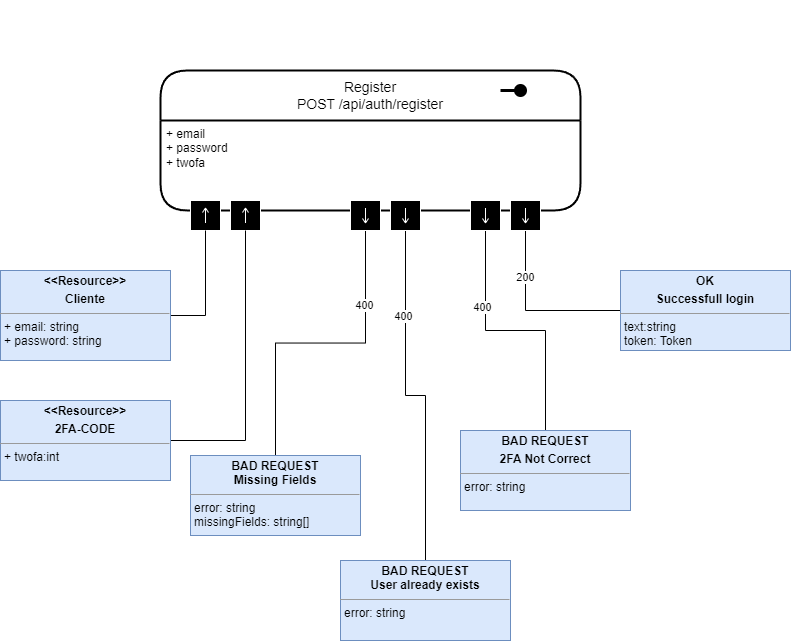
\includegraphics[width=1\textwidth]{images/microservizio-autenticazione/diagrams/diagramma_register.drawio.png}
	\caption{Diagramma dell'endpoint "register"}
\end{figure}


\subsubsection*{Specifica OpenAPI}
Di seguito la specifica openapi dell'endpoint register contenuta nel file 'openapi.yaml' della directory del microservizio
\begin{verbatim}
	/register:
    post:
      summary: Registering method for new users
      description: This endpoint allows new users to register by providing email, password, and two-factor authentication code.
      requestBody:
        required: true
        content:
          application/x-www-form-urlencoded:
            schema:
              type: object
              properties:
                email:
                  type: string
                  format: email
                  
                password:
                  type: string
                  format: password
                twofa:
                  type: string
                  format: twofa-code
              required:
                - email
                - password
                - twofa
      responses:
        '200':
          description: Succesfully registered
          content:
            application/json:
              schema:
                type: object
                properties:
                  text:
                    type: string
                    example: "Successfully registered"
                  token:
                    type: string
                    example: "1231345321532151"
          headers:
            Set-Cookie:
              schema:
                type: string
              description: Session token
        '400':
          description: Bad Request - Missing fields or 2fa not correct or User already exists
          content:
            application/json:
              schema:
                oneOf:
                  - $ref: '#/components/schemas/missingFieldsSchema'
                  - $ref: '#/components/schemas/wrongTwoFaSchema'
                  - $ref: '#/components/schemas/alreadyExistsSchema'

\end{verbatim}

\subsubsection*{Codice}
Questa API viene utilizzata da un utente per creare un proprio account cliente.
Una volta ricevuta la richiesta, viene controllata la presenza di tutti i campi richiesti.
Successivamente si controlla se un utente con la stessa email sia già esistente nel database.
Dopo aver controllato che il codice 2FA sia corretto,viene inserito il nuovo profilo cliente nel database, viene generato un token, aggiunto alla sessione e inviato sia nel body sia come cookie nella risposta.


\begin{figure}[H]
	\centering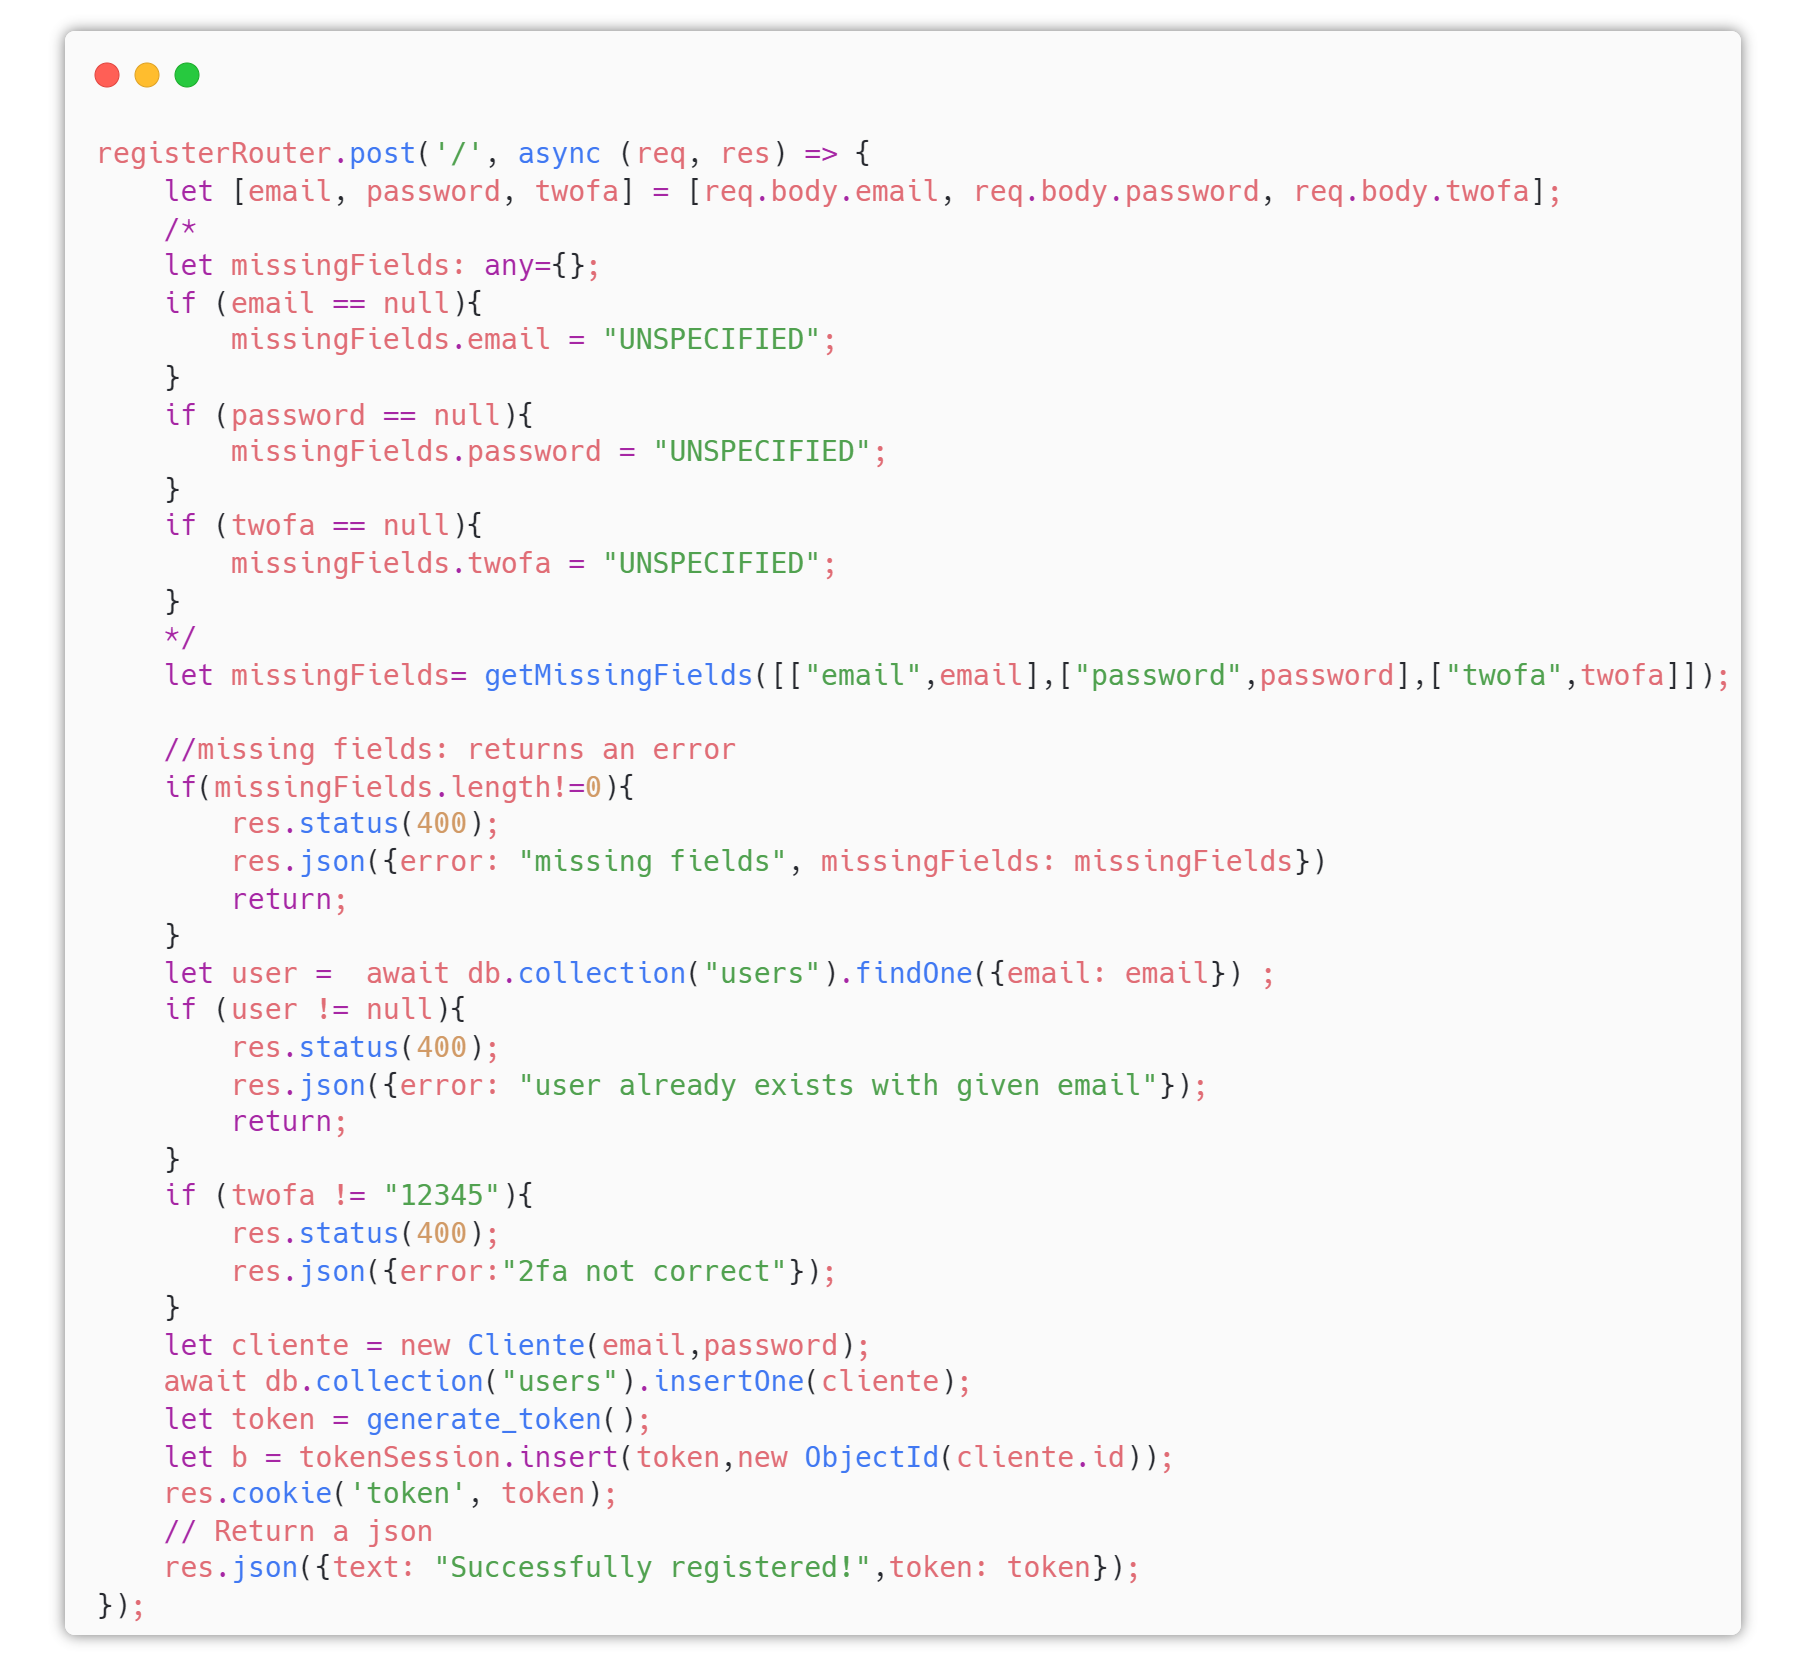
\includegraphics[width=1\textwidth]{images/microservizio-autenticazione/register-carbon.png}
	Codice dell'API api/auth/register
\end{figure}


\subsubsection*{Testing}
Per questo endpoint sono stati creati i seguenti test:

\begin{center} % center the table
	\centering
	\begin{tabular}{ |p{1cm}|p{2cm}|p{2cm}|p{2cm}|p{2cm}|p{1cm}|p{1cm}| }
		\hline
		Numero Testcase & Descrizione Test Case   & Test Data                   & Precondizioni                                  & Dipendenze & Res Atteso & Res Riscontrato \\
		\hline
		1               & Registrato con successo & \{email, password, twofa\}  & email non presente nel sistema, twofa corretto & DB         & 200        & 200             \\
		\hline
		2               & Mancanza campi          & \{ \}                       &                                                &            & 400        & 400             \\
		\hline
		3               & Utente  esistente       & \{ email, password, twofa\} & L'account esiste                               & DB         & 400        & 400             \\
		\hline
	\end{tabular}
\end{center}
\begin{figure}[H]
	\centering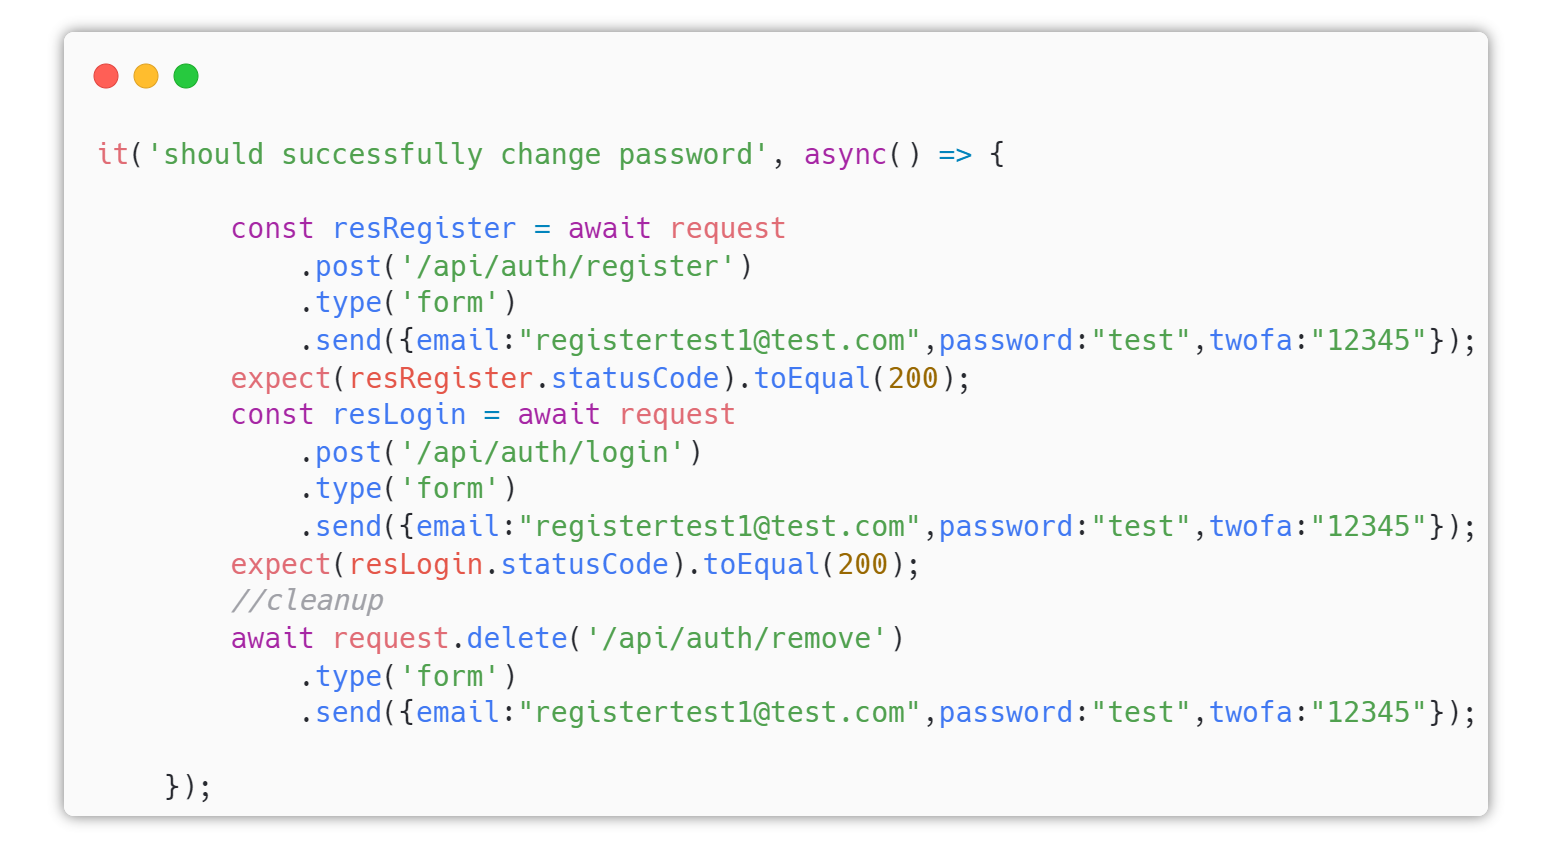
\includegraphics[width=1\textwidth]{images/microservizio-autenticazione/tests/register_test_1.png}
	\caption{Test Register 1}
\end{figure}
\begin{figure}[H]
	\centering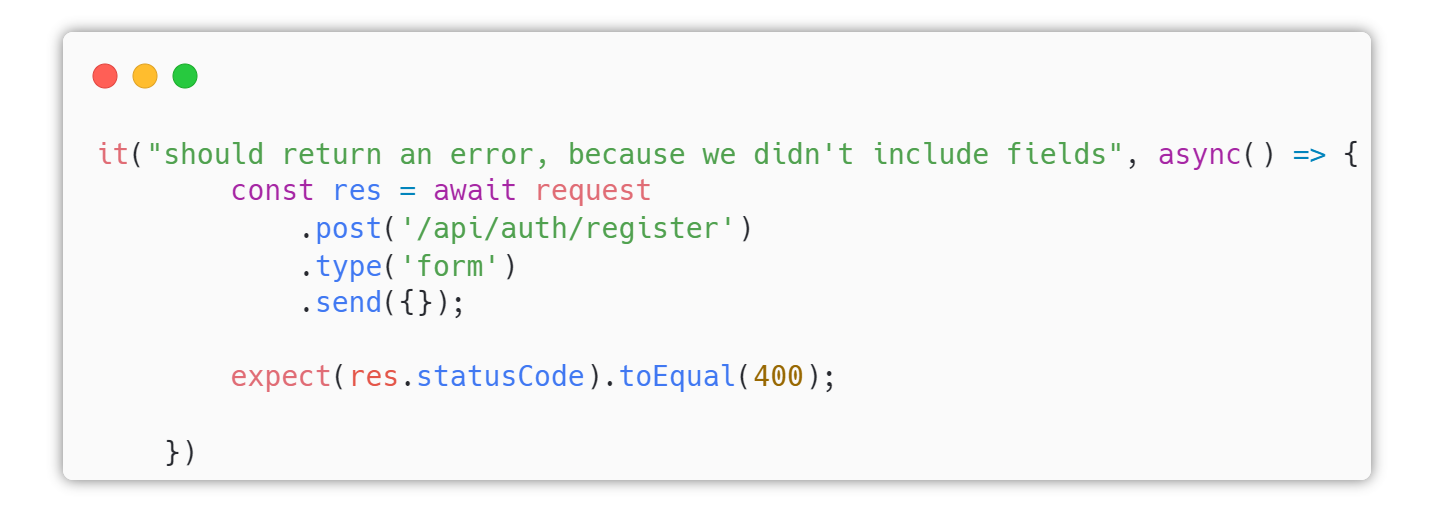
\includegraphics[width=1\textwidth]{images/microservizio-autenticazione/tests/register_test_2.png}
	\caption{Test Register 2}
\end{figure}
\begin{figure}[H]
	\centering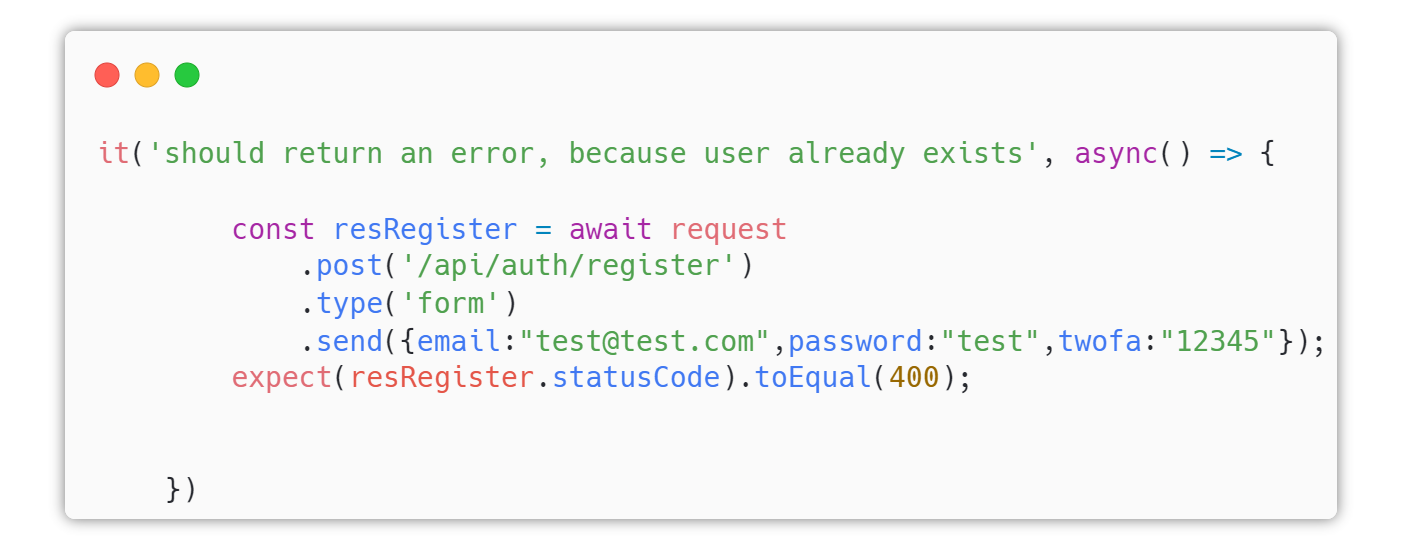
\includegraphics[width=1\textwidth]{images/microservizio-autenticazione/tests/register_test_3.png}
	\caption{Test Register 3}
\end{figure}
I risultati dei test sono i seguenti:
\begin{figure}[H]
	\centering\includegraphics[width=1\textwidth]{images/microservizio-autenticazione/tests/register_test_results.png}
	\caption{Risultati test}
\end{figure}
\subsection{Cambio password}
\subsubsection*{Specifica}
Questa API, all'indirizzo /api/auth/changepass, ha un metodo PATCH e viene utilizzata per cambiare la password di un utente.
La request body è in formato x-www-form-urlencoded e deve contenere i seguenti campi:
\begin{itemize}
	\item email
	\item new\_password
	\item twofa
\end{itemize}
La response body è in formato application/json. Di seguito le possibili risposte:
% table
\begin{center} % center the table
	\centering
	\begin{tabular}{ |p{4cm}|p{5cm}|p{4cm}| }
		\hline
		\centering Status Code & \qquad\quad Body e Cookie                                           & \qquad\qquad Spiegazione                              \\ % I found no other way...
		\hline
		200 OK                 & \{text: "successfully changed your password", token\} cookie: token & Cambio password avvenuto con successo                 \\
		\hline
		400 BAD REQUEST        & \{error: "missing fields", missingFields\}                          & Alcuni campi non sono stati specificati nella request \\ % I found no other way...
		\hline
		404 NOT FOUND          & \{error: "user not found"\}                                         & non esiste utente con la mail fornita                 \\% I found no other way...
		\hline
		400 BAD REQUEST        & \{error: "2fa not correct" \}                                       & Il codice twofa inserito non è corretto.              \\
		\hline
	\end{tabular}
\end{center}
\begin{figure}[H]
	\centering\includegraphics[width=1\textwidth]{images/microservizio-autenticazione/diagrams/diagramma_changepass.drawio.png}
	\caption{Diagramma dell'endpoint "changepass"}
\end{figure}

\subsubsection*{Specifica OpenAPI}
Di seguito la specifica openapi dell'endpoint changepass contenuta nel file 'openapi.yaml'
\begin{verbatim}
	/changepass:
    patch:
      summary: Password Changing Method
      description: This endpoint allows existing users to change their passwords  by providing email, the new password, and two-factor authentication code.
      requestBody:
        required: true
        content:
          application/x-www-form-urlencoded:
            schema:
              type: object
              properties:
                email:
                  type: string
                  format: email
                new_password:
                  type: string
                  format: password
                twofa:
                  type: string
                  format: twofa-code
              required:
                - email
                - new_password
                - twofa
      responses:
        '200':
          description: Successfully changed your password
          content:
            application/json:
              schema:
                type: object
                properties:
                  text:
                    type: string
                    example: "successfully changed your password"
                  token:
                    type: string
                    example: "12312434325321234"
          headers:
            Set-Cookie:
              schema:
                type: string
              description: Session token
        '400':
          description: Bad Request - Missing fields or 2fa not correct
          content:
            application/json:
              schema:
                oneOf:
                  - $ref: '#/components/schemas/missingFieldsSchema'
                  - $ref: '#/components/schemas/wrongTwoFaSchema'
      
        '404':
          description: User not found
          content:
            application/json:
              schema:
                $ref: '#/components/schemas/notFoundSchema'

\end{verbatim}

\subsubsection*{Codice}
Questa API viene utilizzata da un utente per cambiare la password del proprio account.
Una volta ricevuta la richiesta, viene controllata la presenza di tutti i campi richiesti.
Successivamente si controlla se l'utente esista o meno nel database.
Dopo aver controllato che il codice 2FA sia corretto,viene modificata la password nel database, viene generato un token, aggiunto alla sessione e inviato sia nel body sia come cookie nella risposta.

\begin{figure}[H]
	\centering\includegraphics[width=1\textwidth]{images/microservizio-autenticazione/changepass-carbon.png}
	Codice dell'API api/auth/changepass
\end{figure}


\subsubsection*{Testing}
Per questo endpoint sono stati creati i seguenti test:

\begin{center} % center the table
	\centering
	\begin{tabular}{ |p{1cm}|p{2cm}|p{2cm}|p{2cm}|p{2cm}|p{1cm}|p{1cm}| }
		\hline
		Numero Testcase & Descrizione Test Case        & Test Data                       & Precondizioni                                            & Dipendenze & Res Atteso & Res Riscontrato \\
		\hline
		1               & Cambio password con successo & \{email, new\_password, twofa\} & creazione account con richiesta register, twofa corretto & DB         & 200        & 200             \\
		\hline
		2               & Mancanza campi               & \{ \}                           &                                                          &            & 400        & 400             \\
		\hline
	\end{tabular}
\end{center}
\begin{figure}[H]
	\centering\includegraphics[width=1\textwidth]{images/microservizio-autenticazione/tests/password_test_1.png}
	\caption{Test Pass 1}
\end{figure}
\begin{figure}[H]
	\centering\includegraphics[width=1\textwidth]{images/microservizio-autenticazione/tests/password_test_2.png}
	\caption{Test Pass 2}
\end{figure}
I risultati dei test sono i seguenti:
\begin{figure}[H]
	\centering\includegraphics[width=1\textwidth]{images/microservizio-autenticazione/tests/password_test_results.png}
	\caption{Risultati test}
\end{figure}
\subsection{Eliminazione Profilo}
\subsubsection*{Specifica}
Questa API, all'indirizzo /api/auth/remove, ha un metodo POST e viene utilizzata per rimuovere il profilo di un utente.
La request body è in formato x-www-form-urlencoded e deve contenere i seguenti campi:
\begin{itemize}
	\item email
	\item password
	\item twofa
\end{itemize}
La response body è in formato application/json. Di seguito le possibili risposte:
% table
\begin{center} % center the table
	\centering
	\begin{tabular}{ |p{4cm}|p{5cm}|p{4cm}| }
		\hline
		\centering Status Code & \qquad\quad Body e Cookie                                          & \qquad\qquad Spiegazione                              \\ % I found no other way...
		\hline
		200 OK                 & \{text: "successfully removed your account", token\} cookie: token & L'account è stato rimosso con successo                \\
		\hline
		400 BAD REQUEST        & \{error: "missing fields", missingFields\}                         & Alcuni campi non sono stati specificati nella request \\ % I found no other way...
		\hline
		404 NOT FOUND          & \{error: "user not found"\}                                        & non esiste utente con la mail fornita                 \\% I found no other way...
		\hline
		404 NOT FOUND          & \{error: "wrong password" \}                                       & la password inserita non è corretta                   \\
		\hline
		400 BAD REQUEST        & \{error: "2fa not correct" \}                                      & Il codice twofa inserito non è corretto.              \\
		\hline
	\end{tabular}
\end{center}
\begin{figure}[H]
	\centering\includegraphics[width=1\textwidth]{images/microservizio-autenticazione/diagrams/diagramma_remove.drawio.png}
	\caption{Diagramma dell'endpoint "remove"}
\end{figure}

\subsubsection*{Specifica OpenAPI}
Di seguito la specifica openapi dell'endpoint remove contenuta nel file 'openapi.yaml' della directory del microservizio

\begin{verbatim}
	/remove:
    delete:
      summary: Account removal method
      description: This endpoint allows existing users to remove their accounts by providing email, password, and two-factor authentication code.
      requestBody:
        required: true
        content:
          application/x-www-form-urlencoded:
            schema:
              type: object
              properties:
                email:
                  type: string
                  format: email
                password:
                  type: string
                  format: password
                twofa:
                  type: string
                  format: twofa-code
              required:
                - email
                - password
                - twofa
      responses:
        '200':
          description: Succesfully removed the account
          content:
            application/json:
              schema:
                type: object
                properties:
                  text:
                    type: string
                    example: "Successfully removed your account."
        '400':
          description: Bad Request - Missing fields or 2fa not correct
          content:
            application/json:
              schema:
                oneOf:
                  - $ref: '#/components/schemas/missingFieldsSchema'
                  - $ref: '#/components/schemas/wrongTwoFaSchema'
      
        '404':
          description: User not found or wrong password
          content:
            application/json:
              schema:
                oneOf:
                  - $ref: '#/components/schemas/notFoundSchema'
                  - $ref: '#/components/schemas/wrongPassSchema'

\end{verbatim}

\subsubsection*{Codice}
Questa API viene utilizzata da un utente per eliminare il proprio profilo.
Una volta ricevuta la richiesta, viene controllata la presenza di tutti i campi richiesti.
Successivamente si controlla se l'utente esista o meno nel database, e successivamente la validità della password.
Dopo aver controllato che il codice 2FA sia corretto, il profilo viene eliminato dal database e il suo token rimosso dalla sessione.


\begin{figure}[H]
	\centering\includegraphics[width=1\textwidth]{images/microservizio-autenticazione/remove-carbon.png}
	Codice dell'API api/auth/remove
\end{figure}


\subsubsection*{Testing}
Per questo endpoint sono stati creati i seguenti test:
\begin{center} % center the table
	\centering
	\begin{tabular}{ |p{1cm}|p{2cm}|p{2cm}|p{2cm}|p{2cm}|p{1cm}|p{1cm}| }
		\hline
		Numero Testcase & Descrizione Test Case     & Test Data                   & Precondizioni                                               & Dipendenze & Res Atteso & Res Riscontrato \\
		\hline
		1               & Eliminazione con successo & \{email, password, twofa\}  & utente già creato con la richiesta register, twofa corretto & DB         & 200        & 200             \\
		\hline
		2               & Mancanza campi            & \{ \}                       &                                                             &            & 400        & 400             \\
		\hline
		3               & Utente non esiste         & \{ email, password, twofa\} & L'account non esiste                                        & DB         & 404        & 404             \\
		\hline
	\end{tabular}
\end{center}
\begin{figure}[H]
	\centering\includegraphics[width=1\textwidth]{images/microservizio-autenticazione/tests/remove_test_1.png}
	\caption{Test Remove 1}
\end{figure}
\begin{figure}[H]
	\centering\includegraphics[width=1\textwidth]{images/microservizio-autenticazione/tests/remove_test_2.png}
	\caption{Test Remove 2}
\end{figure}
\begin{figure}[H]
	\centering\includegraphics[width=1\textwidth]{images/microservizio-autenticazione/tests/remove_test_3.png}
	\caption{Test Remove 3}
\end{figure}
I risultati dei test sono i seguenti:
\begin{figure}[H]
	\centering\includegraphics[width=1\textwidth]{images/microservizio-autenticazione/tests/remove_test_results.png}
	\caption{Risultati test}
\end{figure}
\subsection{Autentifica Token}
\subsubsection*{Specifica}
Questa API, all'indirizzo/api/auth/authenticate, ha un metodo POST e viene utilizzata da un altro microservizio per autenticare un utente utilizzando il suo token.
La request body è in formato x-www-form-urlencoded e deve contenere il token dell'utente.
La response body è in formato application/json. di seguito le possibili risposte:
% table
\begin{center} % center the table
	\centering
	\begin{tabular}{ |p{4cm}|p{5cm}|p{4cm}| }
		\hline
		\centering Status Code & \qquad\quad Body e Cookie                            & \qquad\qquad Spiegazione                                                                                                     \\ % I found no other way...
		\hline
		200 OK                 & \{text: "success", user\_info: \{permission, id\} \} & L'utente esiste, e ha il seguente id e permissionLevel                                                                       \\
		\hline
		400 BAD REQUEST        & \{error: "missing fields", missingFields\}           & Alcuni campi non sono stati specificati nella request                                                                        \\ % I found no other way...
		\hline
		404 NOT FOUND          & \{error: "user not found with the given token"\}     & non esiste utente nella sessione con il token fornito.                                                                       \\% I found no other way...
		\hline
		404 NOT FOUND          & \{error: "user doesn't exist or is deleted" \}       & Caso impossibile a meno di bug: il token esiste nella sessione, ma l'id utente non corrisponde ad alcun utente del database. \\
		\hline
	\end{tabular}
\end{center}
\begin{figure}[H]
	\centering\includegraphics[width=1\textwidth]{images/microservizio-autenticazione/diagrams/diagramma_auth.drawio.png}
	\caption{Diagramma dell'endpoint "authenticate"}
\end{figure}

\subsubsection*{Specifica OpenAPI}
Di seguito la specifica openapi dell'endpoint authenticate contenuta nel file 'openapi.yaml' della directory del microservizio
\begin{verbatim}
	/authenticate:
    post:
      summary: Method for authentication 
      description: This endpoint allows other microservices to authenticate a user by providing their token
      requestBody:
        required: true
        content:
          application/x-www-form-urlencoded:
            schema:
              type: object
              properties:
                token:
                  type: string
                  
              required:
                  - token
      responses:
        '200':
          description: Success
          content:
            application/json:
              schema:
                type: object
                properties:
                  text:
                    type: string
                    example: "success"
                  user_info:
                    type: object
                    properties:
                      permission:
                        type: string
                        example: "Manager"
                      id:
                        type: string
                        example: "aa231e3421bd1223"

      

        '400':
          description: Bad Request - Missing fields 
          content:
            application/json:
              schema:
                $ref: '#/components/schemas/missingFieldsSchema'
        '404':
          description: User not found with the given token or user doesn't exist 
          content:
            application/json:
              schema:
                oneOf:
                  - $ref: '#/components/schemas/notFoundSchema'
                  - $ref: '#/components/schemas/maybeDeletedSchema'

\end{verbatim}

\subsubsection*{Codice}
Questa API viene utilizzata da un microservizio per autenticare un utente che desidera farne uso.
Una volta ricevuta la richiesta, viene controllata la presenza di tutti i campi richiesti.
Successivamente si controlla se il token fornito abbia un utente corrispondente nella sessione.
Infine il livello di permesso associato all'utente e il suo id vengono inviati nella risposta.
\begin{figure}[H]
	\centering\includegraphics[width=1\textwidth]{images/microservizio-autenticazione/authenticate-carbon.png}
	Codice dell'API api/auth/authenticate
\end{figure}
\subsubsection*{Testing}
Per questo endpoint sono stati creati i seguenti test
\begin{center} % center the table
	\centering
	\begin{tabular}{ |p{1cm}|p{2cm}|p{2cm}|p{2cm}|p{2cm}|p{1cm}|p{1cm}| }
		\hline
		Numero Testcase & Descrizione Test Case         & Test Data  & Precondizioni                     & Dipendenze & Res Atteso & Res Riscontrato \\
		\hline
		1               & Autentificazione con successo & \{token\}  & token presente nella sessione     & DB         & 200        & 200             \\
		\hline
		2               & Mancanza campi                & \{ \}      &                                   &            & 400        & 400             \\
		\hline
		3               & Utente non esiste             & \{ token\} & token non presente nella sessione & DB         & 404        & 404             \\
		\hline
	\end{tabular}
\end{center}
\begin{figure}[H]
	\centering\includegraphics[width=1\textwidth]{images/microservizio-autenticazione/tests/auth_test_1.png}
	\caption{Test Auth 1}
\end{figure}
\begin{figure}[H]
	\centering\includegraphics[width=1\textwidth]{images/microservizio-autenticazione/tests/auth_test_2.png}
	\caption{Test Auth 2}
\end{figure}
\begin{figure}[H]
	\centering\includegraphics[width=1\textwidth]{images/microservizio-autenticazione/tests/auth_test_3.png}
	\caption{Test Auth 3}
\end{figure}
I risultati dei test sono i seguenti:
\begin{figure}[H]
	\centering\includegraphics[width=1\textwidth]{images/microservizio-autenticazione/tests/auth_test_results.png}
	\caption{Risultati test}
\end{figure}
\subsection{Two Factor Authentication}
\subsubsection*{Specifica}
Questa API, all'indirizzo/api/auth/twofa, ha un metodo POST e viene utilizzata da un utente per richiedere un codice 2FA attraverso mail
La request body è in formato x-www-form-urlencoded e deve contenere l'indirizzo email dell'utente.
La response body è in formato application/json. di seguito le possibili risposte:
% table
\begin{center} % center the table
	\centering
	\begin{tabular}{ |p{4cm}|p{5cm}|p{4cm}| }
		\hline
		\centering Status Code & \qquad\quad Body e Cookie                                & \qquad\qquad Spiegazione                              \\ % I found no other way...
		\hline
		200 OK                 & \{text: "Successfully sent the 2FA code to your email"\} & Il codice è stato inviato alla mail correttamente     \\
		\hline
		400 BAD REQUEST        & \{error: "missing fields", missingFields\}               & Alcuni campi non sono stati specificati nella request \\ % I found no other way...
		\hline
	\end{tabular}
\end{center}
\begin{figure}[H]
	\centering\includegraphics[width=1\textwidth]{images/microservizio-autenticazione/diagrams/diagramma_twofa.drawio.png}
	\caption{Diagramma dell'endpoint "changepass"}
\end{figure}


\subsubsection*{Specifica OpenAPI}
Di seguito la specifica openapi dell'endpoint twofa contenuta nel file 'openapi.yaml' della directory del microservizio
\begin{verbatim}
	/twofa:
    post:
      summary: Method for receiving a 2FA code 
      description: This endpoint allows users to request a Two-Factor Authentication code by providing their email
      requestBody:
        required: true
        content:
          application/x-www-form-urlencoded:
            schema:
              type: object
              properties:
                token:
                  type: string
              required:
                  - token
      responses:
        '200':
          description: Succesfully sent the 2FA
          content:
            application/json:
              schema:
                type: object
                properties:
                  text:
                    type: string
                    example: "Successfully sent the 2FA code to your email(SPOILER: IT'S 12345)"
        '400':
          description: Bad Request - Missing fields 
          content:
            application/json:
              schema:
                $ref: '#/components/schemas/missingFieldsSchema'
                     
     
\end{verbatim}

\subsubsection*{Codice}
Questa API viene utilizzata da un utente per ricevere un codice 2FA attraverso email.
Una volta ricevuta la richiesta, viene controllata la presenza di tutti i campi richiesti.
Successivamente viene inviata l'email con il codice 2FA.

\begin{figure}[H]
	\centering\includegraphics[width=1\textwidth]{images/microservizio-autenticazione/twofa-carbon.png}
	Codice dell'API api/auth/twofa
\end{figure}

\subsubsection*{Testing}
Per questo endpoint sono stati creati i seguenti test
\begin{center} % center the table
	\centering
	\begin{tabular}{ |p{1cm}|p{2cm}|p{2cm}|p{2cm}|p{2cm}|p{1cm}|p{1cm}| }
		\hline
		Numero Testcase & Descrizione Test Case      & Test Data & Precondizioni & Dipendenze & Res Atteso & Res Riscontrato \\
		\hline
		1               & Twofa inviato con successo & \{email\} &               &            & 200        & 200             \\
		\hline
		2               & Mancanza campi             & \{ \}     &               &            & 400        & 400             \\
		\hline
	\end{tabular}
\end{center}
\begin{figure}[H]
	\centering\includegraphics[width=1\textwidth]{images/microservizio-autenticazione/tests/twofa_test_1.png}
	\caption{TwoFa Testing 1}
\end{figure}
\begin{figure}[H]
	\centering\includegraphics[width=1\textwidth]{images/microservizio-autenticazione/tests/twofa_test_2.png}
	\caption{TwoFa Testing 2}
\end{figure}
I risultati dei test sono i seguenti:
\begin{figure}[H]
	\centering\includegraphics[width=1\textwidth]{images/microservizio-autenticazione/tests/twofa_test_results.png}
	\caption{Risultati test}
\end{figure}






\section{Frontend}

Questa sezione comprende lo sviluppo e la documentazione del frontend del Microservizio Autenticazione

\subsection{Struttura del frontend}
La struttura del frontend del microservizio autenticazione è riportata
nella figura sotto.
\begin{figure}[H]
	\centering\includegraphics[width=0.5\textwidth]{images/microservizio-autenticazione/frontend-structure.png}
	\caption{Output del comando "tree" all'interno del microservizio autenticazione.}
\end{figure}

\begin{figure}[H]
	\centering\includegraphics[width=1\textwidth]{images/microservizio-autenticazione/frontend/app-carbon.png}
	Codice del componente "App.tsx"
\end{figure}
\subsubsection*{Specifica}
Tutte le componenti facenti parte del microservizio "Autenticazione" vengono gestite dalla componente "App.tsx", quest'ultimo stabilisce gli indirizzi di ciascuna pagina del microservizio e quale componente deve gestire l'indirizzo. 

\subsection{UserFlow}
Lo userflow del microservizio autenticazione viene mostrato sotto nel suo intero. Verrà successivamente suddiviso ed analizzato in ciascun suo componente.
\begin{figure}[H]
	\centering\includegraphics[width=1\textwidth]{images/microservizio-autenticazione/userflow-autenticazione.png}
	\caption{UserFlow del microservizio "Autenticazione"}
\end{figure}


\subsection{Login}

\begin{figure}[H]
	\centering\includegraphics[width=1\textwidth]{images/microservizio-autenticazione/frontend/accesso.jpg}
	\caption{Schermata per il login}
\end{figure}
\subsubsection*{Specifica}
La pagina si occupa di chiedere le credenziali necessarie per effettuare l'accesso nel proprio profilo.\\
E' possibile tornare indietro cliccando il bottone rosso "Cancella"\\
Dopo avere inserito le credenziali è possibile continuare cliccando il bottone verde "Accedi"

\subsubsection*{Userflow}
Partendo dalla pagina "Homepage" l'utente non autenticato deve prima cliccare il tasto "Profilo" presente nella "navbar", successivamente può inserire le proprie credenziali e passare alla pagina "Two Factor Authentication"
\begin{figure}[H]
	\centering\includegraphics[width=1\textwidth]{images/microservizio-autenticazione/frontend/accesso-userflow.png}
	Userflow della pagina "Login"
\end{figure}

\subsubsection*{Codice}
La pagina "Login" è composta da due componenti chiamati "login.tsx" e "formLogin.tsx" con le seguenti caratteristiche:
\begin{itemize}
	\item login.tsx
	\begin{itemize}
		\item Contiene al suo interno "formLogin.tsx"
		\item Contiene controlli e "Fallbacks" per eventuali errori
	\end{itemize}
	\item formLogin.tsx
	\begin{itemize}
		\item Contiene al suo interno un modulo che deve essere compilato dall'utente inserendo l'email e la password.
		\item Contiene controlli sulle credenziali inserite
		\begin{figure}[H]
			\centering\includegraphics[width=1\textwidth]{images/microservizio-autenticazione/frontend/formLogin-carbon.png}
			Codice del componente "formLogin.tsx"
		\end{figure}
	\end{itemize}
\end{itemize}

\subsubsection*{Testing}
Aggiornare la pagina non provoca alcun cambiamento nel comportamento del software.\\Inserire credenziali non valide del tipo:
\begin{itemize}
	\item Spazi vuoti
	\item Numero elevato di caratteri
\end{itemize}
non causa problemi di alcun tipo e vengono gestiti correttamente.


\subsection{Registrazione}

\begin{figure}[H]
	\centering\includegraphics[width=1\textwidth]{images/microservizio-autenticazione/frontend/registrazione.jpg}
	Schermata per la registrazione
\end{figure}
\subsubsection*{Specifica}
La pagina si occupa di chiedere le credenziali necessarie per la creazione di un nuovo profilo per l'utente.\\
E' possibile tornare indietro cliccando il bottone rosso "Cancella"\\
Dopo avere inserito le credenziali è possibile continuare cliccando il bottone verde "Registrati"

\subsubsection*{Userflow}
Partendo dalla pagina "Homepage" l'utente non autenticato deve prima cliccare il tasto "Profilo" presente nella "navbar", successivamente può inserire le proprie credenziali e passare alla pagina "Two Factor Authentication"
\begin{figure}[H]
	\centering\includegraphics[width=1\textwidth]{images/microservizio-autenticazione/frontend/registrazione-userflow.png}
	Userflow della pagina "Registrazione"
\end{figure}

\subsubsection*{Codice}
La pagina "Registrazione" è composta da due componenti chiamati "register.tsx" e "formRegister.tsx" con le seguenti caratteristiche:
\begin{itemize}
	\item register.tsx
	\begin{itemize}
		\item Contiene al suo interno "formRegister.tsx"
		\item Contiene controlli e "Fallbacks" per eventuali errori
	\end{itemize}
	\item formRegister.tsx
	\begin{itemize}
		\item Contiene al suo interno un modulo che deve essere compilato dall'utente inserendo l'email, la password ed una ripetizione della password.
		\item Contiene controlli sulle credenziali inserite
		\begin{figure}[H]
			\centering\includegraphics[width=1\textwidth]{images/microservizio-autenticazione/frontend/formRegister-carbon.png}
			Codice del componente "formRegister.tsx"
		\end{figure}
	\end{itemize}
\end{itemize}

\subsubsection*{Testing}
Aggiornare la pagina non provoca alcun cambiamento nel comportamento del software.\\Inserire credenziali non valide del tipo:
\begin{itemize}
	\item Spazi vuoti
	\item Numero elevato di caratteri
\end{itemize}
non causa problemi di alcun tipo e vengono gestiti correttamente.


\subsection{Two Factor Authentication}

\begin{figure}[H]
	\centering\includegraphics[width=1\textwidth]{images/microservizio-autenticazione/frontend/twofa.jpg}
	Schermata per il "Two Factor Authentication"
\end{figure}
\subsubsection*{Specifica}
La pagina si occupa di chiedere il codice di autenticazione a due fattori che è stato mandato all'utente.\\
E' possibile tornare indietro cliccando il bottone rosso "Cancella"\\
Dopo avere inserito il codice è possibile continuare cliccando il bottone verde "Conferma"

\subsubsection*{Userflow}
Partendo dalle pagine "Login", "Registrazione" o "Elimina Profilo" l'utente ha la possibilità di tornare indietro cliccando il tasto "Cancella", oppure completare il modulo inserendo il codice ricevuto e successivamente cliccando "Conferma". Se il codice è valido l'utente viene poi riportato nella pagina "Homepage".
\begin{figure}[H]
	\centering\includegraphics[width=1\textwidth]{images/microservizio-autenticazione/frontend/twofa-userflow.png}
	Userflow della pagina "Two Factor Authentication"
\end{figure}


\subsubsection*{Codice}
La pagina "Two Factor Authentication" è composta da due componenti chiamati "twoFa.tsx" e "formTwoFa.tsx" con le seguenti caratteristiche:
\begin{itemize}
	\item twoFa.tsx
	\begin{itemize}
		\item Contiene al suo interno "formTwoFa.tsx"
		\item Contiene controlli e "Fallbacks" per eventuali errori
		\begin{figure}[H]
			\centering\includegraphics[width=1\textwidth]{images/microservizio-autenticazione/frontend/twoFa-carbon.png}
			Codice del componente "twoFa.tsx"
		\end{figure}
	\end{itemize}
	\item formTwoFa.tsx
	\begin{itemize}
		\item Contiene al suo interno un modulo che deve essere compilato dall'utente inserendo il codice di autenticazione a due fattori
		\item Contiene controlli sul codice inserito dall'utente
		\begin{figure}[H]
			\centering\includegraphics[width=1\textwidth]{images/microservizio-autenticazione/frontend/formTwoFa-carbon.png}
			Codice del componente "formTwoFa.tsx"
		\end{figure}
	\end{itemize}
\end{itemize}

\subsubsection*{Testing}
Aggiornare la pagina non provoca alcun cambiamento nel comportamento del software.\\Inserire codici non validi del tipo:
\begin{itemize}
	\item Caratteri Speciali
	\item Spazi vuoti
	\item Numero elevato di caratteri
\end{itemize}
non causa problemi di alcun tipo e vengono gestiti correttamente.

\subsection{Profilo}

\begin{figure}[H]
	\centering\includegraphics[width=1\textwidth]{images/microservizio-autenticazione/frontend/profilo.jpg}
	\caption{Schermata per il profilo quando si è autenticati}
\end{figure}
\begin{figure}[H]
	\centering\includegraphics[width=1\textwidth]{images/microservizio-autenticazione/frontend/nonautenticato.jpg}
	\caption{Schermata per il profilo quando non si è autenticati}
\end{figure}
\subsubsection*{Specifica}
La pagina può assumere due aspetti diversi se chi sta cercando di visualizzare la pagina è autenticato oppure no.
Se non si ha ancora fatto il login la pagina si occupa di informare l'utente che non ha ancora fatto l'accesso, ma che tuttavia sta cercando di visualizzare il proprio profilo\\
E' possibile fare il login cliccando il bottone blu "Login"\\
E' possibile registrarsi cliccando il bottone verde "Registrati"
Se il login è già stato effettuato la pagina si occupa di informare l'utente che ha fatto l'accesso.
E' possibile eliminare il proprio profilo cliccando il bottone rosso "Rimuovi Profilo"\\
E' possibile uscire dal proprio profilo cliccando il bottone verde "Logout"


\subsubsection*{Userflow}
Partendo dalla pagina "Homepage" l'utente deve cliccare il tasto "Profilo" presente nella "navbar".
\begin{figure}[H]
	\centering\includegraphics[width=1\textwidth]{images/microservizio-autenticazione/frontend/profilo-userflow.png}
	Userflow della pagina "Profilo"
\end{figure}

\subsubsection*{Codice}
La pagina "Profilo" è composta da due componenti chiamati "profile.tsx" e "notLoggedIn.tsx" con le seguenti caratteristiche:
\begin{itemize}
	\item profile.tsx
	\begin{itemize}
		\item Contiene al suo interno "notLoggedIn.tsx", "logout.tsx", "remove.tsx"
		\item Se l'utente è autenticato mostra due bottoni "Rimuovi Profilo" e "Logout"
		\item Contiene controlli e "Fallbacks" per eventuali errori
	\end{itemize}
	\item notLoggedIn.tsx
	\begin{itemize}
		\item Mostra all'utente due bottoni "Login" e "Registrati"
		\item Contiene controlli sulle credenziali inserite
		\begin{figure}[H]
			\centering\includegraphics[width=1\textwidth]{images/microservizio-autenticazione/frontend/notLoggedIn-carbon.png}
			Codice del componente "notLoggedIn.tsx"
		\end{figure}
	\end{itemize}
\end{itemize}

\subsubsection*{Testing}
Aggiornare la pagina non provoca alcun cambiamento nel comportamento del software.\\





\chapter{Microservizio Task}

\section{Backend}

Questa sezione comprende lo sviluppo e la documentazione del backend del
"Microservizio Task".

\subsection{Lista delle Risorse}

Segue una lista delle risorse implementate dal microservizio:
\begin{itemize}
	\item "Task": contiene tutte le informazioni e i metodi che appartengono alla classe Task (vedi sotto).
	\item "Crea Task": permette all'utente di creare una nuova task.
	\item "Modifica Stato Task": permette al dipendente o al manager di modificare lo stato di una task.
	\item "Scegli Task": permette al dipendente o al manager di assegnare una task al proprio profilo.
	\item "Get Lista Task In Lavorazione": permette al dipendente o al manager di ottenere la lista delle task con lo status di "In Lavorazione" in formato json.
	\item "Get Lista Task Da Eseguire": permette al dipendente o al manager di ottenere la lista delle task con lo status di "Da Eseguire" in formato json.
	\item "Get Lista Task In Pausa": permette al dipendente o al manager di ottenere la lista delle task con lo status di "In Pausa" in formato json.
	\item "Get Storico Task" permette al dipendente o al manager di ottenere la lista delle task con lo status di "Completata" in formato json. Il dipendente rivecerà le tasks che gli sono state assegnate e che sono completate, mentre il dipendente riceverà in risposta tutte le task completate da ogni dipendente.
\end{itemize}

\subsection{Specifica delle Risorse}

Per ogni risorsa elencata nella sezione precedente, si descrive la risorsa attraverso l'utilizzo di illustrazioni e testo.

\subsection{Task}
\subsubsection*{Specifica}

La risorsa "Task" implementa la classe "Task" vista nel "Documento di Architettura".

\begin{figure}[H]
	\centering\includegraphics[width=1\textwidth]{images/resource_task.png}
	Diagramma della risorsa "Task".
\end{figure}

\subsubsection*{Codice}

Segeue l'implementazione nel linguaggio "Typescript":

\begin{figure}[H]
	\centering\includegraphics[width=1\textwidth]{images/code_task.png}
	File situato in "backend/classes/Task.ts".
\end{figure}

\begin{figure}[H]
	\centering\includegraphics[width=1\textwidth]{images/code_task_magazzino.png}
	File situato in "backend/classes/TaskMagazzino.ts".
\end{figure}

\begin{figure}[H]
	\centering\includegraphics[width=1\textwidth]{images/code_task_negozio.png}
	File situato in "backend/classes/TaskNegozio.ts".
\end{figure}

\begin{figure}[H]
	\centering\includegraphics[width=1\textwidth]{images/code_task_riparazione.png}
	File situato in "backend/classes/TaskRiparazione.ts".
\end{figure}

\begin{figure}[H]
	\centering\includegraphics[width=0.9\textwidth]{images/code_task_supporto.png}

	File situato in "backend/classes/TaskSupporto.ts".
\end{figure}

\begin{figure}[H]
	\centering\includegraphics[width=0.9\textwidth]{images/code_task_assistenza.png}

	File situato in "backend/classes/TaskAssistenza.ts".
\end{figure}

\begin{figure}[H]
	\centering\includegraphics[width=1\textwidth]{images/code_task_feedback.png}
	File situato in "backend/classes/TaskFeedback.ts".
\end{figure}

\subsubsection*{Specifica OpenAPI}

Segue la definizione in OpenAPI specification:

\begin{verbatim}
components:
	schemas:
	    Task:
	        type: object
	        properties:
	            nome:
	                type: string
	                example: "Task di esempio"
	            descrizione:
	                type: string
	                example: "Descrizione del task di esempio"
	            taskTag:
	                type: string
	                enum:
	                    - Negozio
	                    - Riparazione
	                    - Magazzino
	                    - Assistenza
	                    - Feedback
	                example: "Riparazione"
	            taskStatus:
	                type: string
	                enum:
	                    - Da Eseguire
	                    - In Lavorazione
	                    - In Pausa
	                    - Completata
	                example: "In Lavorazione"
	        required:
	            - nome
	            - descrizione
	            - taskTag
	            - taskStatus
	    TaskAssistenza:
	        allOf:
	            - $ref: '#/components/schemas/Task'
	            - type: object
	            properties:
	                emailRichiedente:
	                    type: string
	                    format: email
	                    example: "richiedente@example.com"
	            required:
	                - emailRichiedente
	    TaskFeedback:
	        allOf:
	            - $ref: '#/components/schemas/Task'
	            - type: object
	        properties:
	            ideePerMigliorare:
	                type: string
	                example: "Suggerimenti per migliorare il servizio"
	            disponibilitaAzienda:
	                type: string
	                example: "Disponibilità dell'azienda a migliorare"
	            velocitaRiparazione:
	                type: string
	                example: "8"
	            soddisfazioneRiparazione:
	                type: sting
	                example: 9
	            soddisfazioneSitoWeb:
	                type: string
	                example: 7
	        required:
	        - ideePerMigliorare
	        - disponibilitaAzienda
	        - velocitaRiparazione
	        - soddisfazioneRiparazione
	        - soddisfazioneSitoWeb
	   
	    TaskRiparazione:
	        allOf:
	            - $ref: '#/components/schemas/Task'
	            - type: object
	                properties:
	                    nomeRichiedentee:
	                        type: string
	                        example: "Mario"
	                    cognomeRichiedente:
	                        type: string
	                        example: "Rossi"
	                    emailRichiedente:
	                        type: string
	                        format: email
	                        example: "mario.rossi@example.com"
	                    numeroTelefono:
	                        type: string
	                        example: "391234567890"
	                required:
	                    - nomeRichiedente
	                    - cognomeRichiedente
	                    - emailRichiedente
	                    - numeroTelefono
	    TaskMagazzino:
	        allOf:
	            - $ref: '#/components/schemas/Task'
	            - type: object
	    TaskNegozio:
	        allOf:
	            - $ref: '#/components/schemas/Task'
	            - type: object
\end{verbatim}

\subsection{Scegli Task}
\subsubsection*{Specifica}

La risorsa "Scegli Task", accessibile tramite la route "/api/tasks/scegliTask" permette di assegnare una task ad un dipendente o ad un manager. L'API richiede tutti i seguenti campi:

\begin{itemize}
	\item "token": il codice numerico che identifica una sessione autenticata, ottenuto attraverso il microservizio autenticazione.
	\item "taskId": il codice univoco che identifica una task nel database.
\end{itemize}

La response body `e in formato application/json. Di seguito le possibili risposte:

% table
\begin{center} % center the table
	\centering
	\begin{tabular}{ |p{4cm}|p{4cm}|p{4cm}| }
		\hline
		\centering Status Code & \qquad\qquad\quad Body                             & \qquad\quad Spiegazione                                \\ % I found no other way...
		\hline
		200 OK                 & \{Success: "task assigned to the user" \}          & La procedura è terminata con successo                  \\
		\hline
		400 BAD REQUEST        & \{error: "missing fields", missingFields \}        & I campi richiesti sono mancanti.                       \\
		\hline
		401 UNAUTHORIZED       & \{ error: "User not found with the given token" \} & Il token non è valido                                  \\
		\hline
		403 FORBIDDEN          & \{ error: "User not authorized" \}                 & L'utente non ha permessi elevati per accedere all'API  \\
		\hline
		404 NOT FOUND          & \{ error: "Task not found" \}                      & Non è stata trovata alcuna task con il taskid inviato. \\
		\hline
	\end{tabular}
\end{center}


\begin{figure}[H]
	\centering\includegraphics[width=1\textwidth]{images/scegli_task_model.png}
	Diagramma delle risorse per l'API "Scegli Task".
\end{figure}

\subsubsection*{Specifica OpenAPI}

Di seguito viene derscitta la risorsa secondo OpenAPI specification:


\begin{verbatim}
openapi: 3.0.3
    info:
    title: Scegli Task
    version: 1.0.0
    description: Permette di assegnare una
                 task ad un dipendente o ad un manager
paths:
    /api/tasks/scegliTask:
    post:
        requestBody:
            required: true
            content:
                application/json:
                    schema:
                        type: object
                        properties:
                            token:
                                type: string
                                description: Il token ottenuto attraverso
                                             il microservizio autenticazione.
                                example: 171595638452613
                            taskid:
                                type: string
                                description: L'identificativo univoco
                                             della task
                                example: 66476aa0726f8460bce4a26d
                        required:
                            - token
                            - taskid
        responses:
            '200':
                description: Task assigned to the user
                content:
                    application/json:
                    schema:
                        type: object
                        properties:
                            Success:
                               type: string
                                example: "Task assigned to the user"
            '400':
                description: Bad Request
                content:
                    application/json:
                        schema:
                            type: object
                            properties:
                                error:
                                    type: string
                                    example: "missing fields"
                                missingFields:
                                    type: array
                                    items:
                                    type: string
                                    example: token
                            required:
                                - error
                                - missingFields
            '401':
                description: Unauthorized
                content:
                    application/json:
                        schema:
                            type: object
                            properties:
                                error:
                                    type: string
                                    example: "user not found with
                                              the given token"
                            required:
                               - error
            '403':
                description: Forbidden
                content:
                    application/json:
                        schema:
                            type: object
                                properties:
                                    error:
                                        type: string
                                        example: "User not authorized"
                                    required:
                                        - error
            '404':
                description: Not Found
                content:
                    application/json:
                        schema:
                            type: object
                                properties:
                                    error:
                                        type: string
                                        example: "taskidask not found"
                                required:
                                    - error
	
	
\end{verbatim}

\subsubsection*{Codice}

Il codice che implementa quanto detto sopra è il seguente:

\begin{figure}[H]
	\centering\includegraphics[width=1\textwidth]{images/code_scegli_task.png}
	Codice estratto da "backend/routes/scegliTaskRouter.ts".
\end{figure}
\begin{figure}[H]
	\centering\includegraphics[width=1\textwidth]{images/code_task_exists.png}
	Funzione "taskExists()".
\end{figure}
\begin{figure}[H]
	\centering\includegraphics[width=1\textwidth]{images/code_scegli_task_query.png}
	Funzione "executeQuery()".
\end{figure}

\subsubsection*{Testing}

Sono stati realizzati i seguenti tests per coprire ogni possibile risultato della chiamata:

% table
\begin{center} % center the table
	\centering
	\begin{tabular}{ |p{1cm}|p{2cm}|p{2cm}|p{2cm}|p{2cm}|p{1cm}|p{1cm}| }
		\hline
		Numero Testcase & Descrizione Test Case                    & Test Data                                      & Precondizioni                         & Dipendenze                       & Res Atteso & Res Riscontrato \\
		\hline
		1               & Nessun field                             & -                                              & -                                     & -                                & 400        & 400             \\
		\hline
		2               & Invio Token non valido                   & \{token: "fake" \}                             & -                                     & -                                & 401        & 401             \\
		\hline
		3               & Invio Token da un cliente                & \{ token: tokenCliente \}                      & Esistenza di un cliente nel DB        & Microservizio Autenticazione, DB & 403        & 403             \\
		\hline
		4               & Invio di un token valido ma senza taskid & \{ token: tokenManager \}                      & Esistenza di un manager nel DB        & Microservizio Autenticazione, DB & 400        & 400             \\
		\hline
		5               & Invio token valido, taskid non valido    & \{ token: tokenManager, taskid: "fake" \}      & Esistenza di un Manager nel DB        & Microservizio Autenticazione, DB & 404        & 404             \\
		\hline
		6               & Invio token valido con taskid valido     & \{ token: tokenManager, taskid: validTaskid \} & Esistenza di un Manager e Task nel DB & Microservizio Autenticazione, DB & 200        & 200             \\
		\hline
	\end{tabular}
\end{center}

Di seguito il codice dei tests e l'output:

\begin{figure}[H]
	\centering\includegraphics[width=1\textwidth]{images/code_scegli_task_test1.png}
	Testcase 1
\end{figure}
\begin{figure}[H]
	\centering\includegraphics[width=1\textwidth]{images/code_scegli_task_test2.png}
	Testcase 2
\end{figure}
\begin{figure}[H]
	\centering\includegraphics[width=1\textwidth]{images/code_scegli_task_test3.png}
	Testcase 3
\end{figure}
\begin{figure}[H]
	\centering\includegraphics[width=1\textwidth]{images/code_scegli_task_test4.png}
	Testcase 4
\end{figure}
\begin{figure}[H]
	\centering\includegraphics[width=1\textwidth]{images/code_scegli_task_test5.png}
	Testcase 5
\end{figure}
\begin{figure}[H]
	\centering\includegraphics[width=1\textwidth]{images/code_scegli_task_test6.png}
	Testcase 6
\end{figure}

\begin{figure}[H]
	\centering\includegraphics[width=1\textwidth]{images/jest_scegli_task.png}
	Risultato dei tests
\end{figure}


\subsection{Modifica Stato Task}
\subsubsection*{Specifica}

La risorsa "Modifica Stato Task" è accessibile tramite la route "/api/tasks/modificaStatoTask". Permette al dipendente o al manager di impostare un nuovo stato ad una task presente nel database. Gli stati possibili sono definiti nell'enum TaskStatus e sono i seguenti: "DaEseguire", "InLavorazione", "InPausa". "Completata".

\begin{figure}[H]
	\centering\includegraphics[width=1\textwidth]{images/code_enum_taskStatus.png}

	Definizione dell'enum "TaskStatus" in "backend/enums/TaskStatus.ts".
\end{figure}

La risorsa richiede tutti i seguenti campi nel body:
\begin{itemize}
	\item "taskid": identificativo univoco di una task
	\item "token": token ottenuto dal microservizio autenticazione
	\item "taskStatus": il nuovo stato che verrà impostato nella task
\end{itemize}

Il corpo della risposta è in formato application/json e riporta le seguenti risposte:

\begin{center} % center the table
	\centering
	\begin{tabular}{ |p{4cm}|p{4cm}|p{4cm}| }
		\hline
		\centering Status Code & \qquad\qquad\quad Body                             & \qquad\quad Spiegazione                                                       \\ % I found no other way...
		\hline
		200 OK                 & \{Success: "Task status changed succesfully" \}    & La procedura è terminata con successo                                         \\
		\hline
		400 BAD REQUEST        & \{error: "missing fields", missingFields \}        & I campi richiesti sono mancanti.                                              \\
		\hline
		400 BAD REQUEST        & \{error: "Wrong status", missingFields \}          & Lo status inviato non è valido (non corrisponde ad uno dei valori dell'enum). \\
		\hline
		401 UNAUTHORIZED       & \{ error: "User not found with the given token" \} & Il token non è valido                                                         \\
		\hline
		403 FORBIDDEN          & \{ error: "User not authorized" \}                 & L'utente non ha permessi elevati per accedere all'API                         \\
		\hline
		404 NOT FOUND          & \{ error: "Task not found" \}                      & Non è stata trovata alcuna task con il taskid inviato.                        \\
		\hline
	\end{tabular}
\end{center}

\begin{figure}[H]
	\centering\includegraphics[width=1\textwidth]{images/model_modifica_task.png}

	Modello delle risorse per "/api/tasks/modificaStatoTask".
\end{figure}

\subsubsection*{Specifica OpenAPI}

Segue la definizione secondo OpenAPI:

\begin{verbatim}
openapi: 3.0.3
    info:
    title: Modifica Stato Tas
    version: 1.0.0
paths:
    /api/tasks/modificaStatoTask:
        post:
            summary: Modifica lo stato di una task
            description: Questa route permette al dipendente o al
                         manager di cambiare lo stato di una task.
            requestBody:
                required: true
                content:
                    application/json:
                        schema:
                            type: object
                            properties:
                                token:
                                    type: string
                                    description: Il token dell'utente
                                    example: 171595638452613
                                taskid:
                                    type: string
                                    description: Identificativo della task
                                    example: 66476aa0726f8460bce4a26d
                                taskStatus:
                                    type: TaskStatus
                                    description: Il nuovo stato della task.
                                    example: Completata
                            required:
                                - token
                                - taskid
                                - taskStatus
            responses:
                '200':
                    description: Task status changed successfully
                        content:
                            application/json:
                                schema:
                                    type: objectà
                                    properties:
                                        Success:
                                            type: string
                                            example: "Task status
                                                      changed successfully"
                '400':
                    description: Bad Request
                    content:
                        application/json:
                            schema:
                                type: object
                                properties:
                                    error:
                                        type: string
                                        example: "missing fields"
                                    missingFields:
                                        type: array
                                    items:
                                        type: string
                                required:
                                    - error
                                    - missingFields
                '401':
                    description: Unauthorized
                    content:
                        application/json:
                            schema:
                                type: object
                                properties:
                                    error:
                                        type: string
                                        example: "user not found
                                                  with the given token"
                                required:
                                    - error
                '403':
                    description: Forbidden
                    content:
                        application/json:
                            schema:
                                type: object
                                properties:
                                    error:
                                        type: string
                                        example: "User not authorized"
                                required:
                                    - error
                '404':
                    description: Not Found
                    content:
                        application/json:
                            schema:
                                type: object
                                properties:
                                    error:
                                        type: string
                                        example: "Task not found"
                               required:
                                   - error
\end{verbatim}

\subsubsection*{Codice}

Il codice è il seguente:
\begin{figure}[H]
	\centering\includegraphics[width=0.8\textwidth]{images/code_modifica_stato.png}

	Estratto da "backend/routes/modificaStatoTask".
\end{figure}
\begin{figure}[H]
	\centering\includegraphics[width=0.8\textwidth]{images/code_modifica_stato_query.png}

	Funzione "checkStatus()" e "executeQuery()".
\end{figure}

\subsubsection*{Testing}

Sono stati creati i seguenti tests:

% table
\begin{center} % center the table
	\centering
	\begin{tabular}{ |p{1cm}|p{2cm}|p{2cm}|p{2cm}|p{2cm}|p{1cm}|p{1cm}| }
		\hline
		Numero Testcase & Descrizione Test Case                                           & Test Data                                                               & Precondizioni                         & Dipendenze                       & Res Atteso & Res Riscontrato \\
		\hline
		1               & Nessun field                                                    & -                                                                       & -                                     & -                                & 400        & 400             \\
		\hline
		2               & Invio Token non valido                                          & \{token: "fake" \}                                                      & -                                     & -                                & 401        & 401             \\
		\hline
		3               & Invio Token da un cliente                                       & \{ token: tokenCliente \}                                               & Esistenza di un cliente nel DB        & Microservizio Autenticazione, DB & 403        & 403             \\
		\hline
		4               & Invio di un token valido ma senza taskid                        & \{ token: tokenManager \}                                               & Esistenza di un manager nel DB        & Microservizio Autenticazione, DB & 400        & 400             \\
		\hline
		5               & Invio token valido con taskid valido ma con uno stato sbagliato & \{ token: tokenManager, taskid: validTaskid, taskStatus: "fake" \}      & Esistenza di un Manager e Task nel DB & Microservizio Autenticazione, DB & 400        & 400             \\
		\hline
		6               & Invio token valido con taskid valido e uno stato valido         & \{ token: tokenManager, taskid: validTaskid, taskStatus: validStatus \} & Esistenza di un Manager e Task nel DB & Microservizio Autenticazione, DB & 200        & 200             \\
		\hline
	\end{tabular}
\end{center}

Di seguito il codice dei tests:

\begin{figure}[H]
	\centering\includegraphics[width=0.8\textwidth]{images/code_modifica_stato_test1.png}

	Testcase 1
\end{figure}
\begin{figure}[H]
	\centering\includegraphics[width=0.8\textwidth]{images/code_modifica_stato_test2.png}

	Testcase 2
\end{figure}
\begin{figure}[H]
	\centering\includegraphics[width=0.8\textwidth]{images/code_modifica_stato_test3.png}

	Testcase 3
\end{figure}
\begin{figure}[H]
	\centering\includegraphics[width=0.8\textwidth]{images/code_modifica_stato_test4.png}

	Testcase 4
\end{figure}
\begin{figure}[H]
	\centering\includegraphics[width=0.8\textwidth]{images/code_modifica_stato_test5.png}

	Testcase 5
\end{figure}
\begin{figure}[H]
	\centering\includegraphics[width=0.8\textwidth]{images/code_modifica_stato_test6.png}

	Testcase 6
\end{figure}

\begin{figure}[H]
	\centering\includegraphics[width=0.8\textwidth]{images/jest_modifica_stato.png}

	Risultato dei tests
\end{figure}

\subsection{Get Lista Task In Lavorazione}
\subsubsection*{Specifica}

La risorsa "Get Lista Task In Lavorazione" è accessibile tramite la route

"/api/tasks/getListaTaskInLavorazione". Permette al dipendente o al manager di ottenere una lista in formato json delle task nello stato di "In Lavorazione". Gli elementi della rispecchiano gli attributi della risorsa "Task" vista precedentemente.

La risorsa richiede tutti i seguenti campi nel body:
\begin{itemize}
	\item "token": token ottenuto dal microservizio autenticazione che identifica la sessione
\end{itemize}

Il corpo della risposta è in formato application/json e riporta le seguenti risposte:

\begin{center} % center the table
	\centering
	\begin{tabular}{ |p{4cm}|p{4cm}|p{4cm}| }
		\hline
		\centering Status Code & \qquad\qquad\quad Body                             & \qquad\quad Spiegazione                               \\ % I found no other way...
		\hline
		200 OK                 & \{ [ task1, task2, ... ] \}                        & La procedura è terminata con successo                 \\
		\hline
		400 BAD REQUEST        & \{error: "missing fields", missingFields \}        & I campi richiesti sono mancanti o malformati.         \\
		\hline
		401 UNAUTHORIZED       & \{ error: "User not found with the given token" \} & Il token non è valido                                 \\
		\hline
		403 FORBIDDEN          & \{ error: "User not authorized" \}                 & L'utente non ha permessi elevati per accedere all'API \\
		\hline
	\end{tabular}
\end{center}

\begin{figure}[H]
	\centering\includegraphics[width=1\textwidth]{images/model_in_lavorazione.png}

	Modello delle risorse per "/api/tasks/getListaTaskInLavorazione".
\end{figure}

\subsubsection*{Specifica OpenAPI}

\begin{verbatim}
openapi: 3.0.3
info:
     title: Get Lista Task In lavorazione
     description: API getListaTaskInLavorazione
     version: 1.0.0
paths:
    /api/tasks/getListaTaskInLavorazione:
        post:
            summary: Ritorna tutte le tasks on lo stato di "In Lavorazione"
            requestBody:
                required: true
                content:
                    application/json:
                        schema:
                            type: object
                            properties:
                                token:
                                    type: string
                                    description: User's authentication token
                                    example: 171595638452613
                            required:
                                - token
            responses:
                '200':
                    description: Successfully retrieved tasks in progress
                    content:
                        application/json:
                            schema:
                                type: array
                                items:
                                    $ref: '#/components/schemas/TaskInLavorazione'

                '400':
                    description: Missing fields in the request
                    content:
                        application/json:
                            schema:
                                type: object
                                properties:
                                    error:
                                        type: string
                                        example: missing fields
                                        missingFields:
                                            type: array
                                            items:
                                               type: string
                                               example: token
                '401':
                    description: User not found with the given token
                    content:
                        application/json:
                            schema:
                                type: object
                                properties:
                                    error:
                                        type: string
                                        example: user not found with the given token
                '403':
                    description: User not authorized
                    content:
                        application/json:
                            schema:
                                type: object
                                properties:
                                    error:
                                        type: string
                                        example: User not authorized

\end{verbatim}

\subsubsection*{Codice}

Il codice che implementa quanto sopra è il seguente:

\begin{figure}[H]
	\centering\includegraphics[width=1\textwidth]{images/code_in_lavorazione.png}

	Codice estratto da "backend/routes/getListaTaskInLavorazione".
\end{figure}
\begin{figure}[H]
	\centering\includegraphics[width=1\textwidth]{images/code_in_lavorazione2.png}
\end{figure}

\subsubsection*{Testing}

Sono stati individuati i seguenti test cases:

% table
\begin{center} % center the table
	\centering
	\begin{tabular}{ |p{1cm}|p{2cm}|p{2cm}|p{2cm}|p{2cm}|p{1cm}|p{1cm}| }
		\hline
		Numero Testcase & Descrizione Test Case     & Test Data                 & Precondizioni                         & Dipendenze                       & Res Atteso & Res Riscontrato \\
		\hline
		1               & Nessun field              & -                         & -                                     & -                                & 400        & 400             \\
		\hline
		2               & Invio Token non valido    & \{token: "fake" \}        & -                                     & -                                & 401        & 401             \\
		\hline
		3               & Invio Token da un cliente & \{ token: tokenCliente \} & Esistenza di un cliente nel DB        & Microservizio Autenticazione, DB & 403        & 403             \\
		\hline
		4               & Invio token valido        & \{ token: tokenManager \} & Esistenza di un Manager e Task nel DB & Microservizio Autenticazione, DB & 200        & 200             \\
		\hline
	\end{tabular}
\end{center}

Di seguito il codice dei suddetti tests:

\begin{figure}[H]
	\centering\includegraphics[width=1\textwidth]{images/code_in_lavorazione_test1.png}

	Testcase 1
\end{figure}
\begin{figure}[H]
	\centering\includegraphics[width=1\textwidth]{images/code_in_lavorazione_test2.png}

	Testcase 2
\end{figure}
\begin{figure}[H]
	\centering\includegraphics[width=1\textwidth]{images/code_in_lavorazione_test3.png}

	Testcase 3
\end{figure}
\begin{figure}[H]
	\centering\includegraphics[width=1\textwidth]{images/code_in_lavorazione_test4.png}

	Testcase 4
\end{figure}

\begin{figure}[H]
	\centering\includegraphics[width=1\textwidth]{images/jest_in_lavorazione.png}

	Risultato dei tests
\end{figure}

\subsection{Get Lista Task Da Eseguire}
\subsubsection*{Specifica}

La risorsa "Get Lista Task Da Eseguire" è accessibile tramite la route

"/api/tasks/getListaTaskDaEdeguire". Permette al dipendente o al manager di ottenere una lista in formato json delle task nello stato di "Da Eseguire". Gli elementi della rispecchiano gli attributi della risorsa "Task" vista precedentemente.

La risorsa richiede tutti i seguenti campi nel body:
\begin{itemize}
	\item "token": token ottenuto dal microservizio autenticazione che identifica la sessione
\end{itemize}

Il corpo della risposta è in formato application/json e riporta le seguenti risposte:

\begin{center} % center the table
	\centering
	\begin{tabular}{ |p{4cm}|p{4cm}|p{4cm}| }
		\hline
		\centering Status Code & \qquad\qquad\quad Body                             & \qquad\quad Spiegazione                               \\ % I found no other way...
		\hline
		200 OK                 & \{ [ task1, task2, ... ] \}                        & La procedura è terminata con successo                 \\
		\hline
		400 BAD REQUEST        & \{error: "missing fields", missingFields \}        & I campi richiesti sono mancanti o malformati.         \\
		\hline
		401 UNAUTHORIZED       & \{ error: "User not found with the given token" \} & Il token non è valido                                 \\
		\hline
		403 FORBIDDEN          & \{ error: "User not authorized" \}                 & L'utente non ha permessi elevati per accedere all'API \\
		\hline
	\end{tabular}
\end{center}

\begin{figure}[H]
	\centering\includegraphics[width=1\textwidth]{images/model_da_eseguire.png}

	Modello delle risorse per "/api/tasks/getListaTaskDaEseguire".
\end{figure}

\subsubsection*{Specifica OpenAPI}

\begin{verbatim}
openapi: 3.0.3
info:
    title: Get Lista Task Da Eseguire
	description: API getListaTaskDaEseguire
	version: 1.0.0
paths:
	/api/tasks/getListaTaskDaEseguire:
	    post:
	        summary: Ritorna tutte le tasks on lo stato di "Da Eseguire"
	        requestBody:
	            required: true
	            content:
	                application/json:
	                    schema:
	                        type: object
	                        properties:
	                            token:
	                                type: string
	                                description: User's authentication token
	                                example: 171595638452613
	                        required:
	                            - token
	    responses:
	        '200':
	            description: Successfully retrieved tasks in progress
	            content:
	                application/json:
	                    schema:
	                        type: array
	                        items:
	                            $ref: '#/components/schemas/TaskInLavorazione'
	        '400':
	            description: Missing fields in the request
	            content:
	                application/json:
	                    schema:
	                        type: object
	                        properties:
	                            error:
	                                type: string
	                                example: missing fields
	                            missingFields:
	                                type: array
	                                items:
	                                    type: string
	                                    example: token
	        '401':
	            description: User not found with the given token
	            content:
	                application/json:
	                    schema:
	                        type: object
	                        properties:
	                            error:
	                                type: string
	                                example: user not found with the given token
	        '403':
	            description: User not authorized
	            content:
	                application/json:
	                    schema:
	                    type: object
	                    properties:
	                        error:
	                        type: string
	                        example: User not authorized
	
\end{verbatim}

\subsubsection*{Codice}

Il codice è il seguente:
\begin{figure}[H]
	\centering\includegraphics[width=1\textwidth]{images/code_da_eseguire.png}

	Codice estratto da "backend/routes/getListaTaskDaEseguire".
\end{figure}
\begin{figure}[H]
	\centering\includegraphics[width=1\textwidth]{images/code_da_eseguire2.png}
\end{figure}

\subsubsection*{Testing}

Sono stati creati i seguenti test cases:
% table
\begin{center} % center the table
	\centering
	\begin{tabular}{ |p{1cm}|p{2cm}|p{2cm}|p{2cm}|p{2cm}|p{1cm}|p{1cm}| }
		\hline
		Numero Testcase & Descrizione Test Case     & Test Data                 & Precondizioni                         & Dipendenze                       & Res Atteso & Res Riscontrato \\
		\hline
		1               & Nessun field              & -                         & -                                     & -                                & 400        & 400             \\
		\hline
		2               & Invio Token non valido    & \{token: "fake" \}        & -                                     & -                                & 401        & 401             \\
		\hline
		3               & Invio Token da un cliente & \{ token: tokenCliente \} & Esistenza di un cliente nel DB        & Microservizio Autenticazione, DB & 403        & 403             \\
		\hline
		4               & Invio token valido        & \{ token: tokenManager \} & Esistenza di un Manager e Task nel DB & Microservizio Autenticazione, DB & 200        & 200             \\
		\hline
	\end{tabular}
\end{center}

Di seguito il loro codice:

\begin{figure}[H]
	\centering\includegraphics[width=1\textwidth]{images/code_da_eseguire_test1.png}

	Testcase 1
\end{figure}
\begin{figure}[H]
	\centering\includegraphics[width=1\textwidth]{images/code_da_eseguire_test2.png}

	Testcase 2
\end{figure}
\begin{figure}[H]
	\centering\includegraphics[width=1\textwidth]{images/code_da_eseguire_test3.png}

	Testcase 3
\end{figure}
\begin{figure}[H]
	\centering\includegraphics[width=1\textwidth]{images/code_da_eseguire_test4.png}

	Testcase 4
\end{figure}

\begin{figure}[H]
	\centering\includegraphics[width=1\textwidth]{images/jest_da_eseguire.png}

	Risultato tests
\end{figure}

\subsection{Get Lista Task In Pausa}
\subsubsection*{Specifica}


La risorsa "Get Lista Task In Pausa" è accessibile tramite la route

"/api/tasks/getListaTaskInPausa". Permette al dipendente o al manager di ottenere una lista in formato json delle task nello stato di "In Pausa". Gli elementi della rispecchiano gli attributi della risorsa "Task" vista precedentemente.

La risorsa richiede tutti i seguenti campi nel body:
\begin{itemize}
	\item "token": token ottenuto dal microservizio autenticazione che identifica la sessione
\end{itemize}

Il corpo della risposta è in formato application/json e riporta le seguenti risposte:

\begin{center} % center the table
	\centering
	\begin{tabular}{ |p{4cm}|p{4cm}|p{4cm}| }
		\hline
		\centering Status Code & \qquad\qquad\quad Body                             & \qquad\quad Spiegazione                               \\ % I found no other way...
		\hline
		200 OK                 & \{ [ task1, task2, ... ] \}                        & La procedura è terminata con successo                 \\
		\hline
		400 BAD REQUEST        & \{error: "missing fields", missingFields \}        & I campi richiesti sono mancanti o malformati.         \\
		\hline
		401 UNAUTHORIZED       & \{ error: "User not found with the given token" \} & Il token non è valido                                 \\
		\hline
		403 FORBIDDEN          & \{ error: "User not authorized" \}                 & L'utente non ha permessi elevati per accedere all'API \\
		\hline
	\end{tabular}
\end{center}

\begin{figure}[H]
	\centering\includegraphics[width=1\textwidth]{images/model_in_pausa.png}

	Modello delle risorse per "/api/tasks/getListaTaskInPausa".
\end{figure}

\subsubsection*{Specifica OpenAPI}

\begin{verbatim}
openapi: 3.0.3
    info:
    title: Get Lista Task In Pausa
    edescription: API getListaTaskInPausa
version: 1.0.0
paths:
    /api/tasks/getListaTaskInPausa:
        post:
            summary: Ritorna tutte le tasks on lo stato di "In Pausa"
            requestBody:
                required: true
                content:
                    application/json:
                        schema:
                            type: object
                            properties:
                                token:
                                    type: string
                                    description: User's authentication token
                                    example: 171595638452613
                            required:
                                - token
        responses:
            '200':
                description: Successfully retrieved tasks in progress
                content:
                    application/json:
                        schema:
                            type: array
                            items:
                                $ref: '#/components/schemas/TaskInLavorazione'
            '400':
                description: Missing fields in the request
                content:
                    application/json:
                        schema:
                            type: object
                            properties:
                                error:
                                    type: string
                                    example: missing fields
                                missingFields:
                                    type: array
                                    items:
                                        type: string
                                        example: token
            '401':
                description: User not found with the given token
                content:
                    application/json:
                        schema:
                            type: object
                            properties:
                                error:
                                    type: string
                                    example: user not found with the given token
            '403':
                description: User not authorized
                content:
                    application/json:
                        schema:
                            type: object
                            properties:
                                error:
                                    type: string
                                    example: User not authorized
\end{verbatim}

\subsubsection*{Codice}

Il codice è quanto segue:
\begin{figure}[H]
	\centering\includegraphics[width=1\textwidth]{images/code_in_pausa.png}

	Codice estratto da "backend/routes/getlistaTaskInPausa".
\end{figure}
\begin{figure}[H]
	\centering\includegraphics[width=1\textwidth]{images/code_in_paus2.png}
\end{figure}

\subsubsection*{Testing}

Sono stati creati i seguenti test cases:
% table
\begin{center} % center the table
	\centering
	\begin{tabular}{ |p{1cm}|p{2cm}|p{2cm}|p{2cm}|p{2cm}|p{1cm}|p{1cm}| }
		\hline
		Numero Testcase & Descrizione Test Case     & Test Data                 & Precondizioni                         & Dipendenze                       & Res Atteso & Res Riscontrato \\
		\hline
		1               & Nessun field              & -                         & -                                     & -                                & 400        & 400             \\
		\hline
		2               & Invio Token non valido    & \{token: "fake" \}        & -                                     & -                                & 401        & 401             \\
		\hline
		3               & Invio Token da un cliente & \{ token: tokenCliente \} & Esistenza di un cliente nel DB        & Microservizio Autenticazione, DB & 403        & 403             \\
		\hline
		4               & Invio token valido        & \{ token: tokenManager \} & Esistenza di un Manager e Task nel DB & Microservizio Autenticazione, DB & 200        & 200             \\
		\hline
	\end{tabular}
\end{center}

\begin{figure}[H]
	\centering\includegraphics[width=1\textwidth]{images/code_in_pausa_test1.png}

	Testcase 1
\end{figure}
\begin{figure}[H]
	\centering\includegraphics[width=1\textwidth]{images/code_in_pausa_test2.png}

	Testcase 2
\end{figure}
\begin{figure}[H]
	\centering\includegraphics[width=1\textwidth]{images/code_in_pausa_test3.png}

	Testcase 3
\end{figure}
\begin{figure}[H]
	\centering\includegraphics[width=1\textwidth]{images/code_in_pausa_test4.png}

	Testcase 4
\end{figure}

\begin{figure}[H]
	\centering\includegraphics[width=1\textwidth]{images/jest_in_pausa.png}

	Risultato dei tests.
\end{figure}

\subsection{Get Storico Task}
\subsubsection*{Specifica}

La risorsa "Get Storico Task" è accessibile tramite la route

"/api/tasks/getStoricoTask". Permette al dipendente o al manager di ottenere una lista in formato json delle task nello stato di "Completata". Gli elementi della rispecchiano gli attributi della risorsa "Task" vista precedentemente.
Il dipendente otterrà solo le task alle quali è stato assegnato, mentre il manager otterrà tutte le task completate presenti nel database.

La risorsa richiede tutti i seguenti campi nel body:
\begin{itemize}
	\item "token": token ottenuto dal microservizio autenticazione che identifica la sessione
\end{itemize}

Il corpo della risposta è in formato application/json e riporta le seguenti risposte:

\begin{center} % center the table
	\centering
	\begin{tabular}{ |p{4cm}|p{4cm}|p{4cm}| }
		\hline
		\centering Status Code & \qquad\qquad\quad Body                             & \qquad\quad Spiegazione                               \\ % I found no other way...
		\hline
		200 OK                 & \{ [ task1, task2, ... ] \}                        & La procedura è terminata con successo                 \\
		\hline
		400 BAD REQUEST        & \{error: "missing fields", missingFields \}        & I campi richiesti sono mancanti o malformati.         \\
		\hline
		401 UNAUTHORIZED       & \{ error: "User not found with the given token" \} & Il token non è valido                                 \\
		\hline
		403 FORBIDDEN          & \{ error: "User not authorized" \}                 & L'utente non ha permessi elevati per accedere all'API \\
		\hline
	\end{tabular}
\end{center}


\begin{figure}[H]
	\centering\includegraphics[width=1\textwidth]{images/model_storico_task.png}

	Modello delle risorse per "/api/tasks/getStoricoTask".
\end{figure}

\subsubsection*{Specifica OpenAPI}
\begin{verbatim}
openapi: 3.0.3
    info:
    title: Get Storico Task
    description: API getStoricoTask
version: 1.0.0
paths:
    /api/tasks/getStoricoTask:
        post:
            summary: Ritorna tutte le tasks on lo stato di "Completate"
            requestBody:
            required: true
                content:
                    application/json:
                        schema:
                        type: object
                        properties:
                            token:
                                type: string
                                description: User's authentication token
                                example: 171595638452613
                        required:
                            - token
        responses:
            '200':
                description: Successfully retrieved tasks in progress
                content:
                    application/json:
                        schema:
                            type: array
                            items:
                                $ref: '#/components/schemas/TaskInLavorazione'
            '400':
                description: Missing fields in the request
                content:
                    application/json:
                        schema:
                            type: object
                            properties:
                                error:
                                    type: string
                                    example: missing fields
                                missingFields:
                                    type: array
                                    items:
                                        type: string
                                        example: token
            '401':
                description: User not found with the given token
                content:
                    application/json:
                        schema:
                            type: object
                            properties:
                                error:
                                    type: string
                                    example: user not found with the given token
            '403':
                description: User not authorized
                content:
                    application/json:
                        schema:
                            type: object
                            properties:
                                error:
                                    type: string
                                    example: User not authorized
\end{verbatim}
\subsubsection*{Codice}

Il codice è il seguente:
\begin{figure}[H]
	\centering\includegraphics[width=1\textwidth]{images/code_storico.png}

	Estratto di codice dal file "backend/routes/getStoricoTask".
\end{figure}
\begin{figure}[H]
	\centering\includegraphics[width=1\textwidth]{images/code_storico2.png}
\end{figure}

\subsubsection*{Testing}

Sono stati individuati i seguenti test cases:
% table
\begin{center} % center the table
	\centering
	\begin{tabular}{ |p{1cm}|p{2cm}|p{2cm}|p{2cm}|p{2cm}|p{1cm}|p{1cm}| }
		\hline
		Numero Testcase & Descrizione Test Case     & Test Data                 & Precondizioni                         & Dipendenze                       & Res Atteso & Res Riscontrato \\
		\hline
		1               & Nessun field              & -                         & -                                     & -                                & 400        & 400             \\
		\hline
		2               & Invio Token non valido    & \{token: "fake" \}        & -                                     & -                                & 401        & 401             \\
		\hline
		3               & Invio Token da un cliente & \{ token: tokenCliente \} & Esistenza di un cliente nel DB        & Microservizio Autenticazione, DB & 403        & 403             \\
		\hline
		4               & Invio token valido        & \{ token: tokenManager \} & Esistenza di un Manager e Task nel DB & Microservizio Autenticazione, DB & 200        & 200             \\
		\hline
	\end{tabular}
\end{center}

\begin{figure}[H]
	\centering\includegraphics[width=1\textwidth]{images/code_storico_test1.png}

	Testcase 1
\end{figure}
\begin{figure}[H]
	\centering\includegraphics[width=1\textwidth]{images/code_storico_test2.png}

	Testcase 2
\end{figure}
\begin{figure}[H]
	\centering\includegraphics[width=1\textwidth]{images/code_storico_test3.png}

	Testcase 3
\end{figure}
\begin{figure}[H]
	\centering\includegraphics[width=1\textwidth]{images/code_storico_test4.png}

	Testcase 4
\end{figure}

\begin{figure}[H]
	\centering\includegraphics[width=1\textwidth]{images/jest_storico.png}

	Testcase 4
\end{figure}


\subsection{Crea Task}
\subsubsection*{Specifica}

La risorsa "Crea Task" è accessibile tramite la route

"/api/tasks/creaTask". Permette a chiunque sia autenticato di creare una task. L'oggetto task da creare deve essere compatibile con il costruttore di una delle classi che ereditano la risorsa "Task" definita precedentemente.

La risorsa richiede tutti i seguenti campi nel body:
\begin{itemize}
	\item "token": token ottenuto dal microservizio autenticazione che identifica la sessione
\end{itemize}

Il corpo della risposta è in formato application/json e riporta le seguenti risposte:

\begin{center} % center the table
	\centering
	\begin{tabular}{ |p{4cm}|p{4cm}|p{4cm}| }
		\hline
		\centering Status Code & \qquad\qquad\quad Body                             & \qquad\quad Spiegazione                               \\ % I found no other way...
		\hline
		200 OK                 & \{ Seccess: "task created" \}                      & La procedura è terminata con successo                 \\
		\hline
		400 BAD REQUEST        & \{error: "missing fields", missingFields \}        & I campi richiesti sono mancanti o malformati.         \\
		\hline
		401 UNAUTHORIZED       & \{ error: "User not found with the given token" \} & Il token non è valido                                 \\
		\hline
		403 FORBIDDEN          & \{ error: "User not authorized" \}                 & L'utente non ha permessi elevati per accedere all'API \\
		\hline
	\end{tabular}
\end{center}
\begin{figure}[H]
	\centering\includegraphics[width=1\textwidth]{images/model_crea_task.png}

	Modello delle risorse per "/api/tasks/creaTask".
\end{figure}

\subsubsection*{Specifica OpenAPI}
\begin{verbatim}

openapi: 3.0.3
    info:
    title: API Crea Task
    description: API pre /api/tasks/creaTask
    version: 1.0.0
paths:
    /api/tasks/creaTask:
        post:
            summary: Create a task
            description: Questa route permette agli utenti
                         autenticati di creare una nuova task
            requestBody:
                required: true
                content:
                    application/json:
                         schema:
                             oneOf:
                                 - $ref: '#/components/schemas/TaskAssistenza'
                                 - $ref: '#/components/schemas/TaskFeedback'
                                 - $ref: '#/components/schemas/TaskRiparazione'
                                 - $ref: '#/components/schemas/TaskMagazzino'
                                 - $ref: '#/components/schemas/TaskNegozio'
        responses:
            '200':
                description: Successfully created the task
                content:
                    application/json:
                        schema:
                            type: object
                            properties:
                                Success:
                                    type: string
                                    example: "class created"
            '400':
                description: Missing fields in the request
                content:
                    application/json:
                        schema:
                            type: object
                            properties:
                                error:
                                    type: string
                                    example: missing fields
                                missingFields:
                                    type: array
                                    items:
                                        type: string
            '401':
                description: User not found with the given token
                content:
                    application/json:
                        schema:
                            type: object
                            properties:
                                error:
                                    type: string
                                    example: User not found
                                             with the given token

\end{verbatim}

\subsubsection*{Codice}

Il codice è il seguente:
\begin{figure}[H]
	\centering\includegraphics[width=1\textwidth]{images/code_crea_task.png}

	Estratto di codice dal file "backend/routes/creaTask".
\end{figure}
\begin{figure}[H]
	\centering\includegraphics[width=1\textwidth]{images/code_crea_task2.png}
\end{figure}
\begin{figure}[H]
	\centering\includegraphics[width=1\textwidth]{images/code_crea_task3.png}
\end{figure}
\begin{figure}[H]
	\centering\includegraphics[width=1\textwidth]{images/code_crea_task4.png}
\end{figure}

\subsubsection*{Testing}
Sono stati individuati i seguenti test cases:
% table
\begin{center} % center the table
	\centering
	\begin{tabular}{ |p{1cm}|p{2cm}|p{2cm}|p{2cm}|p{2cm}|p{1cm}|p{1cm}| }
		\hline
		Numero Testcase & Descrizione Test Case                             & Test Data                                                                          & Precondizioni                  & Dipendenze                       & Res Atteso & Res Riscontrato \\
		\hline
		1               & Nessun field                                      & -                                                                                  & -                              & -                                & 400        & 400             \\
		\hline
		2               & Invio Token non valido                            & \{token: "fake" \}                                                                 & -                              & -                                & 401        & 401             \\
		\hline
		3               & Invio token senza task tag                        & \{ token: validToken \}                                                            & Esistenza Manager nel DB       & Microsetvizio Autenticazione, DB & 400        & 400             \\
		4               & Invio token con task tag sbagliato                & \{ token: validToken, taskTag: "fake" \}                                           & Esistenza Manager nel DB       & Microservizio Autenticazione, DB & 400        & 400             \\
		5               & Invio Token con task tag ma senza altri attributi & \{ token: tokenCliente, taskTag: "Magazzino" \}                                    & Esistenza di un cliente nel DB & Microservizio Autenticazione, DB & 400        & 400             \\
		\hline
		6               & Tutto valido                                      & \{ token: tokenManager, taskTak: "Magazzino", nome: "test", descrizione: "test" \} & Esistenza di un Manager nel DB & Microservizio Autenticazione, DB & 200        & 200             \\
		\hline
	\end{tabular}
\end{center}

Codice dei testcases:

\begin{figure}[H]
	\centering\includegraphics[width=1\textwidth]{images/code_crea_task_test1.png}

	Testcase 1
\end{figure}
\begin{figure}[H]
	\centering\includegraphics[width=1\textwidth]{images/code_crea_task_test2.png}

	Testcase 2
\end{figure}
\begin{figure}[H]
	\centering\includegraphics[width=1\textwidth]{images/code_crea_task_test3.png}

	Testcase 3
\end{figure}
\begin{figure}[H]
	\centering\includegraphics[width=1\textwidth]{images/code_crea_task_test4.png}

	Testcase 4
\end{figure}
\begin{figure}[H]
	\centering\includegraphics[width=1\textwidth]{images/code_crea_task_test5.png}

	Testcase 5
\end{figure}
\begin{figure}[H]
	\centering\includegraphics[width=1\textwidth]{images/code_crea_task_test6.png}

	Testcase 6
\end{figure}

\begin{figure}[H]
	\centering\includegraphics[width=1\textwidth]{images/jest_crea_task.png}

	Risultato testcases
\end{figure}


\chapter{Microservizio Gestione Dipendenti}
\section{Backend}

Questa sezione comprende lo sviluppo e la documentazione del backend del Microservizio Autenticazione

\subsection*{Struttura del backend}
La struttura del backend del microservizio autenticazione è riportata
nella figura sotto.
\begin{figure}[H]
	\centering\includegraphics[width=0.5\textwidth]{images/microservizio-autenticazione/backend-structure.png}
	\caption{Output del comando "tree" all'interno di un microservizio.}
\end{figure}
\subsection*{Modellazione dati nel database}
\subsection*{Specifica delle Risorse}
Di seguito le risorse estratte dal diagramma delle classi e utilizzate da questo microservizio.
\paragraph*{<<resource>> Dipendente}
Rappresenta il profilo di un Dipendente.
Ha tutti gli attributi di cliente, in più:
\begin{itemize}
	\item nome
	\item cognome
	\item data di assunzione
	\item data di nascita
	\item worktags
\end{itemize}
\paragraph*{Manager}
Rappresenta il profilo del Manager.
Ha tutti gli attributi di Dipendente, ma ha come permissionLevel "Manager"

Metodi
\paragraph*{<<resource>> crea}
Permette al manager di creare un profilo dipendente.
E' un'API del backend
\paragraph*{<<resource>> rimuovi}
Permette al manager di rimuovere un profilo dipendente
E' un'API del backend
\paragraph*{<<resource>> cerca}
Permette al manager di cercare profili dipendente
E' un'API del backend
\paragraph*{<<resource>> storico}
Permette al manager di visualizzare lo storico task di un determinato dipendente
E' un'API del backend

\subsection{Crea profilo Dipendente}

\subsubsection*{Specifica}
Questa API, all'indirizzo /api/dipendenti/create, ha un metodo POST e viene utilizzata per la creazione di un profilo dipendente da parte del Manager.
La request body è in formato x-www-form-urlencoded e deve contenere i seguenti campi:
\begin{itemize}

	\item email
	\item password
	\item data di nascita
	\item data di assunzione
	\item lista worktag
\end{itemize}
Inoltre, per verificare che il manager sia autenticato, il suo token va inserito o all'interno del body o attraverso un cookie.
La response body è in formato application/json. Di seguito le possibili risposte:
% table
\begin{center} % center the table
	\centering
	\begin{tabular}{ |p{4cm}|p{5cm}|p{4cm}| }
		\hline
		\centering Status Code & \qquad\quad Body e Cookie                             & \qquad\qquad Spiegazione                                                             \\ % I found no other way...
		\hline
		200 OK                 & \{text: "successfully created the profile"\}          & Profilo dipendente creato con successo                                               \\
		\hline
		401 UNAUTHORIZED       & \{error: "missing token"\}                            & Il token non è presente nella richiesta                                              \\
		\hline
		403 FORBIDDEN          & \{error: "permission denied"\}                        & Il token è presente nella richiesta, ma l'utente associato non è un manager          \\
		\hline
		404 NOT FOUND          & \{error: "No user found with the given token"\}       & Il token è presente nella richiesta, ma non corrisponde a nessun profilo autenticato \\
		\hline
		400 BAD REQUEST        & \{error: "missing fields", missingFields\}            & Alcuni campi non sono stati specificati nella request                                \\ % I found no other way...
		\hline
		400 BAD REQUEST        & \{error: "user already exists with the given email"\} & Esiste già un utente con la mail fornita                                             \\% I found no other way...
		\hline
		400 BAD REQUEST        & \{error: "invalid birth date" \}                      & La data di nascita fornita non è in un formato riconosciuto                          \\
		\hline
		400 BAD REQUEST        & \{error: "invalid assunzione date" \}                 & La data di assunzione fornita non è in un formato riconosciuto                       \\
		\hline
		400 BAD REQUEST        & \{error: "no worktag array" \}                        & il campo della richiesta 'worktag' non è un array                                    \\
		\hline
		400 BAD REQUEST        & \{error: "elements provided are not worktags" \}      & Gli elementi forniti all'interno di 'worktag' non sono worktags                      \\
		\hline
	\end{tabular}
\end{center}
\begin{figure}[H]
	\centering\includegraphics[width=1\textwidth]{images/microservizio-dipendenti/diagrams/create_diagram.drawio.png}
	\caption{Diagramma dell'endpoint create}
\end{figure}

\subsubsection*{Specifica OpenAPI}
Di seguito la specifica openapi dell'endpoint remove contenuta nel file 'openapi.yaml' della directory del microservizio
\begin{verbatim}
	/create:
    post:
      summary: Metodo per la creazione di profili dipendente da parte del manager
      description: Questo endpoint permette al manager di creare un profilo dipendente fornendo email, password, nome, cognome, data di nascita, data di assunzione, worktag
      requestBody:
        required: true
        content:
          application/x-www-form-urlencoded:
            schema:
              type: object
              properties:
                email:
                  type: string
                  format: email

                password:
                  type: string
                  format: password
                  
                nome:
                  type: string
                cognome:
                  type: string
                nascita:
                  type: string
                  format: date
                assunzione:
                  type: string
                  format: date
                worktag:
                  type: array
                token:
                  type: string
               
              required:
                - email
                - password
                - nome
                - cognome
                - nascita
                - assunzione
                - worktag
                - token
      responses:
        '200':
          description: "Profilo creato con successo"
          content:
            application/json:
              schema:
                type: object
                properties:
                  text:
                    type: string
                    example: "successfully created"
                  
            

        '401':
          description: "Token mancante nella richiesta"
          content:
            application/json:
              schema:
                $ref: "#/components/schemas/missingTokenSchema"
        '403':
          description: "Il token non corrisponde al token del manager"
          content:
            application/json:
              schema:
                $ref: "#/components/schemas/notTheManagerSchema"

        '404':
          description: "Il token non corrisponde a nessun utente"
          content:
            application/json:
              schema:
                $ref: "#/components/schemas/notFoundSchema"
        '400':
          description: Bad Request - 'Missing fields' or 'invalid birth date' or 'invalid assunzione date' or 'no worktag array'or 'elements provided are not worktags' or 'user with given email already exists'
          content:
            application/json:
              schema:
                oneOf:
                  - $ref: '#/components/schemas/missingFieldsSchema'
                  - type: object
                    properties:
                      text:
                        type: string
                        example: 
                          oneOf:
                            - "invalid birth date"
                            - "invalid assunzione date"
                  - type: object
                    properties:
                      text:
                        type: string
                        example:
                          oneOf:
                            - "no worktag array"
                            - "elements provided are not worktags"
                  - $ref: '#/components/schemas/alreadyExistsSchema'
\end{verbatim}
\subsubsection*{Codice}
Questa api viene utilizzata dal manager per la creazione di un profilo dipendente.
Una volta ricevuta la richiesta, viene controllata inizialmente la presenza del token del manager nel body o nel token attraverso il middleware 'permissionMiddleware'.
Successivamente viene controllata la presenza di tutti i campi richiesti e dell'integrità dei dati forniti, ossia:
\begin{itemize}
	\item Se la data di nascita è in un formato valido
	\item Se la data di assunzione è in un formato valido
	\item se 'worktag' è un array
	\item se gli elementi di 'worktag' sono esclusivamente worktags
\end{itemize}
Dopodichè viene controllata la presenza di un utente con la mail fornita nel database.
Infine viene creato il dipendente e memorizzato all'interno del database, ritornando una risposta positiva.
%figure here

\begin{figure}[H]
	\centering\includegraphics[width=1\textwidth]{images/microservizio-dipendenti/create-carbon.png}
	\caption{Codice dell'endpoint create}
\end{figure}


\subsubsection*{Testing}
Per questo endpoint sono stati creati i seguenti test:
\begin{center} % center the table
	\centering
	\begin{tabular}{ |p{1cm}|p{2cm}|p{2cm}|p{2cm}|p{2cm}|p{1cm}|p{1cm}| }
		\hline
		Numero Testcase & Descrizione Test Case & Test Data                   & Precondizioni                                          & Dipendenze & Res Atteso & Res Riscontrato \\
		\hline
		1               & Dipendente creato con successo    & \{email, password, nome, cognome, nascita, assunzione, worktag\}  & utente non esistente &  Microservizio Autenticazione,DB         & 200        & 200             \\
		\hline
		2               & Nascita e Assunzione non validi    & \{email, password, nome, cognome, nascita, assunzione, worktag\}  &  &  Microservizio Autenticazione,DB         & 400        & 400           \\
		\hline
		3              & Elementi forniti non sono worktags    & \{email, password, nome, cognome, nascita, assunzione, worktag\}  &  &  Microservizio Autenticazione,DB         & 400        & 400           \\
		\hline
	\end{tabular}
\end{center}

\begin{figure}[H]
	\centering\includegraphics[width=1\textwidth]{images/microservizio-dipendenti/tests/create_test_1.png}
	\caption{Test Case 1}
\end{figure}
\begin{figure}[H]
	\centering\includegraphics[width=1\textwidth]{images/microservizio-dipendenti/tests/create_test_2.png}
	\caption{Test Case 2}
\end{figure}
\begin{figure}[H]
	\centering\includegraphics[width=1\textwidth]{images/microservizio-dipendenti/tests/create_test_3.png}
	\caption{Test Case 3}
\end{figure}
\begin{figure}[H]
	\centering\includegraphics[width=1\textwidth]{images/microservizio-dipendenti/tests/create_test_results.png}
	\caption{Risultati dei test}
\end{figure}
\subsection{Elimina profilo}
\subsubsection*{Specifica}
Questa API, all'indirizzo /api/dipendenti/delete, ha un metodo delete e viene utilizzata per l'eliminazione di un profilo da parte del Manager.
La request body è in formato x-www-form-urlencoded e deve contenere i seguenti campi:
\begin{itemize}
	\item email
\end{itemize}
Inoltre, per verificare che il manager sia autenticato, il suo token va inserito o all'interno del body o attraverso un cookie.
La response body è in formato application/json. Di seguito le possibili risposte:
% table
\begin{center} % center the table
	\centering
	\begin{tabular}{ |p{4cm}|p{5cm}|p{4cm}| }
		\hline
		\centering Status Code & \qquad\quad Body e Cookie                       & \qquad\qquad Spiegazione                                                             \\ % I found no other way...
		\hline
		200 OK                 & \{text: "successfully deleted the profile"\}    & Profilo eliminato con successo                                                       \\
		\hline
		401 UNAUTHORIZED       & \{error: "missing token"\}                      & Il token non è presente nella richiesta                                              \\
		\hline
		403 FORBIDDEN          & \{error: "permission denied"\}                  & Il token è presente nella richiesta, ma l'utente associato non è un manager          \\
		\hline
		404 NOT FOUND          & \{error: "No user found with the given token"\} & Il token è presente nella richiesta, ma non corrisponde a nessun profilo autenticato \\
		\hline
		400 BAD REQUEST        & \{error: "missing fields", missingFields\}      & Alcuni campi non sono stati specificati nella request                                \\ % I found no other way...
		\hline
		404 NOT FOUND          & \{error: "no user with the given email" \}      & Non esiste alcun utente con la mail fornita                                          \\
		\hline
	\end{tabular}
\end{center}
\begin{figure}[H]
	\centering\includegraphics[width=1\textwidth]{images/microservizio-dipendenti/diagrams/delete_diagram.drawio.png}
	\caption{Diagramma dell'endpoint delete}
\end{figure}

\subsubsection*{Specifica OpenAPI}
Di seguito la specifica openapi dell'endpoint remove contenuta nel file 'openapi.yaml' della directory del microservizio
\begin{verbatim}
	/delete:
    delete:
      summary: Metodo per l'eliminazione di un profilo
      description: Questo endpoint permette al manager di eliminare un profilo fornendo la sua mail
      requestBody:
        required: true
        content:
          application/x-www-form-urlencoded:
            schema:
              type: object
              properties:
                email:
                  type: string
                  format: email
                token:
                  type: string
               
              required:
                - email
                - token
      responses:
        '200':
          description: "Profilo elimanto con successo con successo"
          content:
            application/json:
              schema:
                type: object
                properties:
                  text:
                    type: string
                    example: "successfully deleted the profile"
                  
            

        '401':
          description: "Token mancante nella richiesta"
          content:
            application/json:
              schema:
                $ref: "#/components/schemas/missingTokenSchema"
        '403':
          description: "Il token non corrisponde al token del manager"
          content:
            application/json:
              schema:
                $ref: "#/components/schemas/notTheManagerSchema"

        '404':
          description: "'Il token non corrisponde a nessun utente' OR 'Nessun utente trovato con la mail fornita' "
          content:
            application/json:
              schema:
                $ref: "#/components/schemas/notFoundSchema"
        '400':
          description: Bad Request - 'Missing fields' 
          content:
            application/json:
              schema:
                oneOf:
                  - $ref: '#/components/schemas/missingFieldsSchema'
     
\end{verbatim}
\subsubsection*{Codice}
Questa api viene utilizzata dal manager per eliminare un profilo già esistente nel sistema.
Una volta ricevuta la richiesta, viene controllata inizialmente la presenza del token del manager nel body o nel token attraverso il middleware 'permissionMiddleware'.
Successivamente viene controllata la presenza di tutti i campi richiesti.
Dopodichè viene controllato se l'email fornita corrisponde al profilo di un utente.
Infine viene eliminato il profilo all'interno del database, ritornando un esito positivo
%figure here %%
\begin{figure}[H]
	\centering\includegraphics[width=1\textwidth]{images/microservizio-dipendenti/delete-carbon.png}
	\caption{Codice dell'endpoint delete}
\end{figure}


\subsubsection*{Testing}
Per questo endpoint sono stati creati i seguenti test:
\begin{center} % center the table
	\centering
	\begin{tabular}{ |p{1cm}|p{2cm}|p{2cm}|p{2cm}|p{2cm}|p{1cm}|p{1cm}| }
		\hline
		Numero Testcase & Descrizione Test Case & Test Data                   & Precondizioni                                          & Dipendenze & Res Atteso & Res Riscontrato \\
		\hline
		1               & Dipendente eliminato con successo    & \{email\}  & utente  creato con la richiesta create &  Microservizio Autenticazione,DB         & 200        & 200             \\
		\hline
		2               & utente non trovato  & \{email\}  &  &  Microservizio Autenticazione,DB         & 404        & 404           \\
		\hline
		
	\end{tabular}
\end{center}
\begin{figure}[H]
	\centering\includegraphics[width=1\textwidth]{images/microservizio-dipendenti/tests/delete_test_1.png}
	\caption{Test Case 1}
\end{figure}
\begin{figure}[H]
	\centering\includegraphics[width=1\textwidth]{images/microservizio-dipendenti/tests/delete_test_2.png}
	\caption{Test Case 1}
\end{figure}
\begin{figure}[H]
	\centering\includegraphics[width=1\textwidth]{images/microservizio-dipendenti/tests/delete_test_results.png}
	\caption{Risultati dei test}
\end{figure}
\subsection*{Cerca profili}
\subsubsection*{Specifica}
Questa API, all'indirizzo /api/dipendenti/find, ha un metodo post e viene utilizzata per la ricerca di uno o più profili da parte del manager.
La request body è in formato x-www-form-urlencoded e deve contenere i seguenti campi:
\begin{itemize}
	\item mode
\end{itemize}
il campo mode può assumere i valori 'one' o 'many', e indica se la ricerca debba ritornare uno o più profili.
Il body può contenere, ma non è obbligatorio, i seguenti campi per una ricerca più specifica:
\begin{itemize}
	\item email
	\item nome
	\item cognome
	\item data di nascita
	\item data di assunzione
	\item worktags
\end{itemize}
Inoltre, per verificare che il manager sia autenticato, il suo token va inserito o all'interno del body o attraverso un cookie.
La response body è in formato application/json. Di seguito le possibili risposte:
% table
\begin{center} % center the table
	\centering
	\begin{tabular}{ |p{4cm}|p{5cm}|p{4cm}| }
		\hline
		\centering Status Code & \qquad\quad Body e Cookie                       & \qquad\qquad Spiegazione                                                                           \\ % I found no other way...
		\hline
		200 OK                 & \{user: {...}\}                                 & La ricerca con mode = "one" ha riportato un risultato                                              \\
		\hline
		200 OK                 & \{users: [user1,user2,user3...]\}               & La ricerca con mode = 'many' ha riportato uno o più risultati                                      \\
		\hline
		401 UNAUTHORIZED       & \{error: "missing token"\}                      & Il token non è presente nella richiesta                                                            \\
		\hline
		403 FORBIDDEN          & \{error: "permission denied"\}                  & Il token è presente nella richiesta, ma l'utente associato non è un manager                        \\
		\hline
		404 NOT FOUND          & \{error: "No user found with the given token"\} & Il token è presente nella richiesta, ma non corrisponde a nessun profilo autenticato               \\
		\hline
		400 BAD REQUEST        & \{error: "missing fields", missingFields\}      & Alcuni campi non sono stati specificati nella request                                              \\ % I found no other way...
		\hline
		404 NOT FOUND          & \{error: "no user found" \}                     & Non esiste alcun utente avente i parametri di ricerca forniti. viene ritornato solo con mode = one \\
		\hline
	\end{tabular}
\end{center}
\begin{figure}[H]
	\centering\includegraphics[width=1\textwidth]{images/microservizio-dipendenti/diagrams/find_diagram.drawio.png}
	\caption{Diagramma dell'endpoint find}
\end{figure}

\subsubsection*{Specifica OpenAPI}
Di seguito la specifica openapi dell'endpoint remove contenuta nel file 'openapi.yaml' della directory del microservizio
\begin{verbatim}
	/find:
    post:
      summary: Metodo per la ricerca di profili dipendente da parte del manager
      description: Questo endpoint permette al manager di cercare profili dipendente fornendo email, password, nome, cognome, data di nascita, data di assunzione, worktag
      requestBody:
        required: true
        content:
          application/x-www-form-urlencoded:
            schema:
              type: object
              properties:
                email:
                  type: string
                  format: email

                password:
                  type: string
                  format: password
                  
                nome:
                  type: string
                cognome:
                  type: string
                nascita:
                  type: string
                  format: date
                assunzione:
                  type: string
                  format: date
                worktag:
                  type: array
                token:
                  type: string
                mode: 
                  type: string
                  enum: [one,many]
              required:
                - token
                - mode
      responses:
        '200':
          description: "(mode=one) Profilo trovato OR (mode=many) Profili trovati "
          content:
            application/json:
              schema:
                oneOf:
                  - $ref: '#components/schemas/user'
                  - $ref: '#components/schemas/users'
        '401':
          description: "Token mancante nella richiesta"
          content:
            application/json:
              schema:
                $ref: "#/components/schemas/missingTokenSchema"
        '403':
          description: "Il token non corrisponde al token del manager"
          content:
            application/json:
              schema:
                $ref: "#/components/schemas/notTheManagerSchema"

        '404':
          description: "Il token non corrisponde a nessun utente OR (mode = one) Utente non trovato nella ricerca"
          content:
            application/json:
              schema:
                $ref: "#/components/schemas/notFoundSchema"
        '400':
          description: Bad Request - 'Missing fields' 
          content:
            application/json:
              schema:
                oneOf:
                  - $ref: '#/components/schemas/missingFieldsSchema'
     
\end{verbatim}
\subsubsection*{Codice}
Questa api viene utilizzata dal manager per cercare uno o più  profili presenti nel sistema.
Una volta ricevuta la richiesta, viene controllata inizialmente la presenza del token del manager nel body o nel token attraverso il middleware 'permissionMiddleware'.
Successivamente viene controllata la presenza di tutti i campi richiesti.
Dopodichè vengono presi tutti i campi opzionali forniti e inseriti nella query di ricerca nel database.
Infine il server risponde con il primo profilo trovato che corrisponde ai criteri di ricerca forniti.
% screen here
\begin{figure}[H]
	\centering\includegraphics[width=1\textwidth]{images/microservizio-dipendenti/find-carbon.png}
	\caption{Codice dell'endpoint find}
\end{figure}


\subsubsection*{Testing}
Per questo endpoint sono stati creati i seguenti test:
\begin{center} % center the table
	\centering
	\begin{tabular}{ |p{1cm}|p{2cm}|p{2cm}|p{2cm}|p{2cm}|p{1cm}|p{1cm}| }
		\hline
		Numero Testcase & Descrizione Test Case & Test Data                   & Precondizioni                                          & Dipendenze & Res Atteso & Res Riscontrato \\
		\hline
		1               & Dipendente trovato con successo & \{email, mode=one\}  & utente esistente &  Microservizio Autenticazione,DB         & 200        & 200             \\
		\hline
		2               & Mode non è 'one' o 'many'   & \{email, mode\}  &  &  Microservizio Autenticazione,DB         & 400        & 400           \\
		\hline
		3              & Utente non trovato   & \{email, mode=one\}  & utente non esistente &  Microservizio Autenticazione,DB         & 404      & 404          \\
		\hline
	\end{tabular}
\end{center}
\begin{figure}[H]
	\centering\includegraphics[width=1\textwidth]{images/microservizio-dipendenti/tests/find_test_1.png}
	\caption{Test Case 1}
\end{figure}
\begin{figure}[H]
	\centering\includegraphics[width=1\textwidth]{images/microservizio-dipendenti/tests/find_test_2.png}
	\caption{Test Case 2}
\end{figure}
\begin{figure}[H]
	\centering\includegraphics[width=1\textwidth]{images/microservizio-dipendenti/tests/find_test_3.png}
	\caption{Test Case 3}
\end{figure}
\begin{figure}[H]
	\centering\includegraphics[width=1\textwidth]{images/microservizio-dipendenti/tests/create_test_results.png}
	\caption{Risultati dei test}
\end{figure}
\subsection*{Storico profili}
\subsubsection*{Specifica}
Questa API, all'indirizzo /api/dipendenti/history, ha un metodo post e viene utilizzata per la visione dello storico task di un determinato dipendente
La request body è in formato x-www-form-urlencoded e deve contenere i seguenti campi:
\begin{itemize}
	\item email
\end{itemize}
Inoltre, per verificare che il manager sia autenticato, il suo token va inserito o all'interno del body o attraverso un cookie.
La response body è in formato application/json. Di seguito le possibili risposte:
% table
\begin{center} % center the table
	\centering
	\begin{tabular}{ |p{4cm}|p{5cm}|p{4cm}| }
		\hline
		\centering Status Code & \qquad\quad Body e Cookie                       & \qquad\qquad Spiegazione                                                             \\ % I found no other way...
		\hline
		200 OK                 & \{[task1,task2,task3...]\}                      & La ricerca ha riportato lo storico task con successo                                 \\
		\hline
		401 UNAUTHORIZED       & \{error: "missing token"\}                      & Il token non è presente nella richiesta                                              \\
		\hline
		403 FORBIDDEN          & \{error: "permission denied"\}                  & Il token è presente nella richiesta, ma l'utente associato non è un manager          \\
		\hline
		404 NOT FOUND          & \{error: "No user found with the given token"\} & Il token è presente nella richiesta, ma non corrisponde a nessun profilo autenticato \\
		\hline
		400 BAD REQUEST        & \{error: "missing fields", missingFields\}      & Alcuni campi non sono stati specificati nella request                                \\ % I found no other way...
		\hline
		404 NOT FOUND          & \{error: "dipendente not found" \}              & Non esiste alcun dipendente avente la mail fornita                                   \\
		\hline
	\end{tabular}
\end{center}
\begin{figure}[H]
	\centering\includegraphics[width=1\textwidth]{images/microservizio-dipendenti/diagrams/history_diagram.drawio.png}
	\caption{Diagramma dell'endpoint history}
\end{figure}

\subsubsection*{Specifica OpenAPI}
Di seguito la specifica openapi dell'endpoint remove contenuta nel file 'openapi.yaml' della directory del microservizio
\begin{verbatim}
	/history:
    post:
      summary: Metodo per la visione dello storico task di un dipendente
      description: Questo endpoint permette al manager di vedere lo storico task di un determinato dipendente.
      requestBody:
        required: true
        content:
          application/x-www-form-urlencoded:
            schema:
              type: object
              properties:
                email:
                  type: string
                  format: email
                token:
                  type: string
               
              required:
                - token
                - email
      responses:
        '200':
          description: "Il dipendente esiste e questo è il suo storico task "
          content:
            application/json:
              schema:
                type: array
                items:
                  type: object
                  
        '401':
          description: "Token mancante nella richiesta"
          content:
            application/json:
              schema:
                $ref: "#/components/schemas/missingTokenSchema"
        '403':
          description: "Il token non corrisponde al token del manager"
          content:
            application/json:
              schema:
                $ref: "#/components/schemas/notTheManagerSchema"

        '404':
          description: "Il token non corrisponde a nessun utente OR Utente non trovato nella ricerca"
          content:
            application/json:
              schema:
                $ref: "#/components/schemas/notFoundSchema"
        '400':
          description: Bad Request - 'Missing fields' 
          content:
            application/json:
              schema:
                oneOf:
                  - $ref: '#/components/schemas/missingFieldsSchema'
\end{verbatim}
\subsubsection*{Codice}
Questa api viene utilizzata dal manager per ottenere lo storico task di un determinato dipendente
Una volta ricevuta la richiesta, viene controllata inizialmente la presenza del token del manager nel body o nel token attraverso il middleware 'permissionMiddleware'.
Successivamente viene controllata la presenza di tutti i campi richiesti.
Dopodichè viene controllata la presenza di un dipendente nel database avente la mail fornita.
Infine il server risponde con lo storico task del dipendente.
\begin{figure}[H]
	\centering\includegraphics[width=1\textwidth]{images/microservizio-dipendenti/history-carbon.png}
	\caption{Codice dell'endpoint history}
\end{figure}

\subsubsection*{Testing}
Per questo endpoint sono stati creati i seguenti test:
\begin{center} % center the table
	\centering
	\begin{tabular}{ |p{1cm}|p{2cm}|p{2cm}|p{2cm}|p{2cm}|p{1cm}|p{1cm}| }
		\hline
		Numero Testcase & Descrizione Test Case & Test Data                   & Precondizioni                                          & Dipendenze & Res Atteso & Res Riscontrato \\
		\hline
		1               & Storico trovato con successo   & \{email\}  & dipendente esistente &  Microservizio Autenticazione,DB         & 200        & 200             \\
		\hline
		2               & Utente non trovato   & \{email\}  &  &  Microservizio Autenticazione,DB         & 404        & 404         \\
		\hline
		
	\end{tabular}
\end{center}

\begin{figure}[H]
	\centering\includegraphics[width=1\textwidth]{images/microservizio-dipendenti/tests/history_test_1.png}
	\caption{Test Case 1}
\end{figure}
\begin{figure}[H]
	\centering\includegraphics[width=1\textwidth]{images/microservizio-dipendenti/tests/history_test_2.png}
	\caption{Test Case 2}
\end{figure}
\begin{figure}[H]
	\centering\includegraphics[width=1\textwidth]{images/microservizio-dipendenti/tests/history_test_results.png}
	\caption{Risultati dei test}
\end{figure}

\chapter{Microservizio Home}

\chapter{Deploy}

In questo capitolo si descrivono i procedimenti per effettuare un deploy dell'applicazione con successo in locale.

\section{Dipendenze}
E' necessario aver installato docker nella macchina host. Se l'host si trova su windows, docker può essere installto tramite "WSL" ("Windows Subsystem for Linux").


\section{Ottenere il codice}
Tutto il codice necessario è presente su github, accessibile tramite \href{https://github.com/orgs/IS-FixMi/repositories}{questo} link (le repo sono private quindi se non si è loggati con il profilo autorizzato si otterrà una 404). In particolare, il codice per eseguire l'infrastruttura si trova in \href{https://github.com/IS-FixMi/fixmi-compose}{"fixmi-compose"}. Al suo interno sono contenute le altre repo dei microservizi in submoduli. Per clonare la repo si sui il comando:
\begin{verbatim}
git clone --recurse-submodules https://github.com/IS-FixMi/fixmi-compose.git
\end{verbatim}
\subsection*{Nota:}
Dato che i moduli da installare sono molti, il team di sviluppo consiglia di scaricare la directory con già i moduli tramite il seguente link TODO.
Successivamente, è possibile estrarre la cartella tramite:
\begin{verbatim}
tar -xf archive.tar.gz
\end{verbatim}

\section{Istruzioni}
L'intera infrastruttura può essere eseguita tramite il seguente comando all'interno della cartella "fixmi-compose":
\begin{verbatim}
sudo docker compose up --build
\end{verbatim}
si consiglia di utilizzare quest'ultimo in quanto vengono di impostare tutte le porte e volumi necessari per il corretto funzionamento dell'applicazione.
\subsection*{Problemi Noti}
\begin{itemize}
	\item L'applicazione risulta parecchio pesante, dunque il tempo di download potrebbe essere prolisso.
	\item Sono noti dei problemi nell'installazione dei moduli "concurrently" e "react-scripts". Qualora vi siano dei problemi del tipo "concurrently non è stato trovato", si proceda in questo modo:
	      \begin{enumerate}
		      \item Si entri nella cartella del microservizio che riporta il problema
		      \item Si esegua il comando "npm i <nome-del-modulo-non-trovato> ."
	      \end{enumerate}
	\item Qualora le porte da 3001 a 3008 risultassero già occupate da altri servizi nella macchina host, queste possono essere cambiate nel file "docker-compose.yaml", così come la porta del reverse proxy (7777) e gli ip dei microservizi.
\end{itemize}

\section{Eseguire Singoli Microservizi}
Nonostante eseguire parti dell'infrastruttura indipendenti senza docker compose non sia consigliato, questa sezione riporta le istruzioni per eseguire in microservizio singolarmente e informazioni per il developement.

\subsection*{Microservizio con Docker}
Per eseguire un signolo microservizio dobbiamo buildare il docker container, questo può essere fatto con il seguente comando:
\begin{verbatim}
cd fixmi-microservizio-<nome-del-microservizio>
docker build -t example-microservice .
\end{verbatim}
Successivamente, il docker container può essere eseguito con il comando:
\begin{verbatim}
docker run -p <backend_port>:3001 -p <frontend_port>:3002 \\
-v .:/app example-microservice
\end{verbatim}
\begin{itemize}
	\item Al comando può essere aggiunta la flag "-d" per eseguire il container in detached mode, nascondendo l'output nel background. Si ricordi che per fermare il container sarà necessario usare il comando "docker stop <container-id>" e per leggere i logs si può usare il comando "docker logs <container-id>"
\end{itemize}

\subsection*{Microservizio senza docker}
Per eseguire un microservizio senza l'utilizzo di docker è necessario aver installato "npm". I seguenti comandi sono utili per il deploy e lo sviluppo.
Prima di tutto è necessario installare i moduli da cui dipende il programma:
\begin{verbatim}
npm install .
\end{verbatim}
Il microservizio può essere eseguito in production con:
\begin{verbatim}
npm run buildfront
npm run production
\end{verbatim}
Per eseguire solo la backend:
\begin{verbatim}
npm run startback
\end{verbatim}
Per eseguire solo la frontend:
\begin{verbatim}
npm run startfront
\end{verbatim}
Per eseguire la backend e frontend in dev mode:
\begin{verbatim}
npm run start
\end{verbatim}
Nota: i microservizi utilizzano il database per il salvataggio e la lettura dei dati, e il reverse proxy per ottenere il token di sessione e are redirect agli altri microservizi.

Per qualsiasi problema e assistenza, si contatti um membro dello sviluppo.




\end{document}

